% Options for packages loaded elsewhere
\PassOptionsToPackage{unicode}{hyperref}
\PassOptionsToPackage{hyphens}{url}
\PassOptionsToPackage{dvipsnames,svgnames,x11names}{xcolor}
%
\documentclass[
  letterpaper,
  DIV=11,
  numbers=noendperiod,
  oneside]{scrreprt}

\usepackage{amsmath,amssymb}
\usepackage{lmodern}
\usepackage{iftex}
\ifPDFTeX
  \usepackage[T1]{fontenc}
  \usepackage[utf8]{inputenc}
  \usepackage{textcomp} % provide euro and other symbols
\else % if luatex or xetex
  \usepackage{unicode-math}
  \defaultfontfeatures{Scale=MatchLowercase}
  \defaultfontfeatures[\rmfamily]{Ligatures=TeX,Scale=1}
\fi
% Use upquote if available, for straight quotes in verbatim environments
\IfFileExists{upquote.sty}{\usepackage{upquote}}{}
\IfFileExists{microtype.sty}{% use microtype if available
  \usepackage[]{microtype}
  \UseMicrotypeSet[protrusion]{basicmath} % disable protrusion for tt fonts
}{}
\makeatletter
\@ifundefined{KOMAClassName}{% if non-KOMA class
  \IfFileExists{parskip.sty}{%
    \usepackage{parskip}
  }{% else
    \setlength{\parindent}{0pt}
    \setlength{\parskip}{6pt plus 2pt minus 1pt}}
}{% if KOMA class
  \KOMAoptions{parskip=half}}
\makeatother
\usepackage{xcolor}
\usepackage[left=1in,marginparwidth=2.0666666666667in,textwidth=4.1333333333333in,marginparsep=0.3in]{geometry}
\setlength{\emergencystretch}{3em} % prevent overfull lines
\setcounter{secnumdepth}{5}
% Make \paragraph and \subparagraph free-standing
\ifx\paragraph\undefined\else
  \let\oldparagraph\paragraph
  \renewcommand{\paragraph}[1]{\oldparagraph{#1}\mbox{}}
\fi
\ifx\subparagraph\undefined\else
  \let\oldsubparagraph\subparagraph
  \renewcommand{\subparagraph}[1]{\oldsubparagraph{#1}\mbox{}}
\fi


\providecommand{\tightlist}{%
  \setlength{\itemsep}{0pt}\setlength{\parskip}{0pt}}\usepackage{longtable,booktabs,array}
\usepackage{calc} % for calculating minipage widths
% Correct order of tables after \paragraph or \subparagraph
\usepackage{etoolbox}
\makeatletter
\patchcmd\longtable{\par}{\if@noskipsec\mbox{}\fi\par}{}{}
\makeatother
% Allow footnotes in longtable head/foot
\IfFileExists{footnotehyper.sty}{\usepackage{footnotehyper}}{\usepackage{footnote}}
\makesavenoteenv{longtable}
\usepackage{graphicx}
\makeatletter
\def\maxwidth{\ifdim\Gin@nat@width>\linewidth\linewidth\else\Gin@nat@width\fi}
\def\maxheight{\ifdim\Gin@nat@height>\textheight\textheight\else\Gin@nat@height\fi}
\makeatother
% Scale images if necessary, so that they will not overflow the page
% margins by default, and it is still possible to overwrite the defaults
% using explicit options in \includegraphics[width, height, ...]{}
\setkeys{Gin}{width=\maxwidth,height=\maxheight,keepaspectratio}
% Set default figure placement to htbp
\makeatletter
\def\fps@figure{htbp}
\makeatother
\newlength{\cslhangindent}
\setlength{\cslhangindent}{1.5em}
\newlength{\csllabelwidth}
\setlength{\csllabelwidth}{3em}
\newlength{\cslentryspacingunit} % times entry-spacing
\setlength{\cslentryspacingunit}{\parskip}
\newenvironment{CSLReferences}[2] % #1 hanging-ident, #2 entry spacing
 {% don't indent paragraphs
  \setlength{\parindent}{0pt}
  % turn on hanging indent if param 1 is 1
  \ifodd #1
  \let\oldpar\par
  \def\par{\hangindent=\cslhangindent\oldpar}
  \fi
  % set entry spacing
  \setlength{\parskip}{#2\cslentryspacingunit}
 }%
 {}
\usepackage{calc}
\newcommand{\CSLBlock}[1]{#1\hfill\break}
\newcommand{\CSLLeftMargin}[1]{\parbox[t]{\csllabelwidth}{#1}}
\newcommand{\CSLRightInline}[1]{\parbox[t]{\linewidth - \csllabelwidth}{#1}\break}
\newcommand{\CSLIndent}[1]{\hspace{\cslhangindent}#1}

\KOMAoption{captions}{tableheading}
\makeatletter
\makeatother
\makeatletter
\@ifpackageloaded{bookmark}{}{\usepackage{bookmark}}
\makeatother
\makeatletter
\@ifpackageloaded{caption}{}{\usepackage{caption}}
\AtBeginDocument{%
\ifdefined\contentsname
  \renewcommand*\contentsname{Table of contents}
\else
  \newcommand\contentsname{Table of contents}
\fi
\ifdefined\listfigurename
  \renewcommand*\listfigurename{List of Figures}
\else
  \newcommand\listfigurename{List of Figures}
\fi
\ifdefined\listtablename
  \renewcommand*\listtablename{List of Tables}
\else
  \newcommand\listtablename{List of Tables}
\fi
\ifdefined\figurename
  \renewcommand*\figurename{Figure}
\else
  \newcommand\figurename{Figure}
\fi
\ifdefined\tablename
  \renewcommand*\tablename{Table}
\else
  \newcommand\tablename{Table}
\fi
}
\@ifpackageloaded{float}{}{\usepackage{float}}
\floatstyle{ruled}
\@ifundefined{c@chapter}{\newfloat{codelisting}{h}{lop}}{\newfloat{codelisting}{h}{lop}[chapter]}
\floatname{codelisting}{Listing}
\newcommand*\listoflistings{\listof{codelisting}{List of Listings}}
\makeatother
\makeatletter
\@ifpackageloaded{caption}{}{\usepackage{caption}}
\@ifpackageloaded{subcaption}{}{\usepackage{subcaption}}
\makeatother
\makeatletter
\@ifpackageloaded{tcolorbox}{}{\usepackage[many]{tcolorbox}}
\makeatother
\makeatletter
\@ifundefined{shadecolor}{\definecolor{shadecolor}{rgb}{.97, .97, .97}}
\makeatother
\makeatletter
\@ifpackageloaded{sidenotes}{}{\usepackage{sidenotes}}
\@ifpackageloaded{marginnote}{}{\usepackage{marginnote}}
\makeatother
\makeatletter
\makeatother
\ifLuaTeX
  \usepackage{selnolig}  % disable illegal ligatures
\fi
\IfFileExists{bookmark.sty}{\usepackage{bookmark}}{\usepackage{hyperref}}
\IfFileExists{xurl.sty}{\usepackage{xurl}}{} % add URL line breaks if available
\urlstyle{same} % disable monospaced font for URLs
\hypersetup{
  pdftitle={On the Path to Electrically Pumped Organic Lasers},
  pdfauthor={Alexander Dian},
  colorlinks=true,
  linkcolor={blue},
  filecolor={Maroon},
  citecolor={Blue},
  urlcolor={Blue},
  pdfcreator={LaTeX via pandoc}}

\title{On the Path to Electrically Pumped Organic Lasers}
\author{Alexander Dian}
\date{1/31/23}

\begin{document}
\maketitle
\ifdefined\Shaded\renewenvironment{Shaded}{\begin{tcolorbox}[frame hidden, borderline west={3pt}{0pt}{shadecolor}, boxrule=0pt, enhanced, interior hidden, sharp corners, breakable]}{\end{tcolorbox}}\fi

\bookmarksetup{startatroot}

\hypertarget{preface}{%
\chapter*{Preface}\label{preface}}
\addcontentsline{toc}{chapter}{Preface}

\markboth{Preface}{Preface}

\begin{quote}
``Explorers are we, intrepid and bold, out in the wild, amongst wonders
untold. Equipped with our wits, a map, and a snack; we're searching for
fun and we're on the right track!'' - Calvin and Hobbes
\end{quote}

When I first started my honours thesis, I was excited at for what lied
ahead. I was oozing confidence, naively arrogant, that I was going to
achieve so much. While it isn't a thesis worthy of the lofty
expectations, it is completed. And more importantly I learned a lot.

Maybe the best way to get you excited about my thesis, is to tell you
why I was so excited about it when I first started. I'm a
technology-inclined guy. So, I was aware of OLEDs, organic light
emitting diodes, before I was introduced to them in the physics context.
OLEDs were, and still are, everywhere on the forefront of display
technology. You can find them as the screen for every
\href{https://support.apple.com/en-us/HT208191}{modern phone}, or even
on the new \href{https://www.nintendo.com/switch/oled-model/}{Nintendo
OLED Switch} (valued at roughly \$100 more). Or if you go to the any TV
distributor, the OLEDs are clearly the priciest and highest quality
looking
\href{https://www.whathifi.com/best-buys/tvs/best-oled-tvs}{TVs}. If you
wanted a good screen, the device should be using OLEDs -- that much I
knew.

What I didn't know would come next. It never clicked for awhile that
OLEDs were just Organic LEDs. Organic in the sense they are made of
carbon-based molecules. We'll touch on later why that is important. But
I'll spoil the main interesting part of that now. If it is organic, it
is really easy to alter the structure of the molecule to fine-tune the
properties of the OLED. You can likely make the link yourself that this
opens the possibility of doing so much, not only in terms of efficiency
in manufacturing, but also making new things altogether. This is where
the idea for organic lasers came about.

Organic lasers, like regular lasers, but as before made from
carbon-based molecules. If you're a tech person, you might already know
that there aren't any organic lasers on the Coles shelves yet. In fact,
no one has been able to make organic lasers (at the time of writing).
Again, it'd be rude to giveaway the entire reason why now, but organic
materials have a handicap that makes it difficult to get the energy
output a laser requires.

This is where my thesis comes into it. I set out to, while not exactly
make a laser, but test a very promising organic material and see whether
it meets the lasing requirements. The material,
\href{https://pubchem.ncbi.nlm.nih.gov/compound/2_6-Diphenylanthracene}{2,6-diphenylanthracene
(2,6-DPA)}, is promising because it may exhibit a neat function that may
overcome the handicap that I talked about earlier.

That is about it for an introduction, without getting into the nitty
gritty. But I will include my abstract below with all the jargon in it
for those who want a summary of the above in fewer words.

\bookmarksetup{startatroot}

\hypertarget{abstract}{%
\chapter*{Abstract}\label{abstract}}
\addcontentsline{toc}{chapter}{Abstract}

\markboth{Abstract}{Abstract}

\begin{quote}
Lasers have left an indelible mark on science and technology, from
applications ranging from medicine to telecommunications to spectroscopy
-- we are even starting to see laser televisions. To this day, no one
has realised organic laser diodes despite the rapid and burgeoning
success of organic semiconductors. This failure is because an organic
laser diode needs to be injected with high current densities to achieve
lasing, a threshold that seems out of reach because of the inherent
losses caused by the non-emissive triplet excited states. Managing these
excited states, or better yet turning them into emissive singlet states,
lies at the focus of realising organic lasers. This thesis will
demonstrate the exciting potential of using triplet-triplet upconversion
-- a process that annihilates two triplets to form the emissive singlets
-- to help reduce the current density threshold. I argue for the lasing
potential of the highly emissive lasing material
3-(2-Benzothiazolyl)-N,N-diethylumbelliferylamine (Coumarin6) when doped
into 2,6-diphenylanthracene (2,6-DPA) that herein is confirmed to
exhibit triplet-triplet upconversion.
\end{quote}

\bookmarksetup{startatroot}

\hypertarget{acknowledgements}{%
\chapter*{Acknowledgements}\label{acknowledgements}}
\addcontentsline{toc}{chapter}{Acknowledgements}

\markboth{Acknowledgements}{Acknowledgements}

pic.twitter.com/jiI6k0xJzF

--- BREADSWORD ((\textbf{BREADSWORD?})) July 26, 2022

This thesis could not be completed without the invaluable support I
received from others. I'll begin by thanking my supervisors
A/Prof.~Ebinazar Namdas, A/Prof Shih-Chun Lo (Lawrence), and Dr Atul
Shukla. Each of these individuals have tolerated my shenanigans
throughout the year. Without their patience and expertise, I would not
be where I am today. Similarly, thank you to the COPE team for listening
to me ramble and struggle my way through this thesis.

I want to next thank my family who have always got my back. To my
mother, even though I may waterboard you with nonsense physics, the
calls and conversations you have endured do not go underappreciated. To
my father, your work ethic has inspired me to always keep pushing, even
when this thesis seemed unobtainable ''Dad would have kept going, so
will I'', I would think. To the brothers of mine, the Civil Trio, I now
have this huge document, I guess -- I don't recommend it. I love you
all.

To my family away from home, Tamar Street. You've kept me humble by
reminding me to ''leave the thinking to the intellectuals''; you've
reminded me to relax and have fun in a year of doubt and stress; you've
pushed me to do the things I love and be more of myself than ever. Sam
with basketball, Spencer with gym, Will with yarns, Doug with F1, Laura
with movies, Mia with intellectual-discussions, Sarah with yard-bevvies,
Nicola with gossip, Cass with mental-support: all of you are fantastic.

To myself, well done, bud. You got there. Not the way we imagined at the
start, but we finished. Remember why you did this, but don't forget what
you learned while doing this.

Trust The Process.

\bookmarksetup{startatroot}

\hypertarget{introduction-to-organic-semiconductor-laser-diodes}{%
\chapter[Introduction to organic semiconductor laser
diodes]{\texorpdfstring{\protect\hypertarget{sec:level1}{}{}Introduction
to organic semiconductor laser
diodes}{Introduction to organic semiconductor laser diodes}}\label{introduction-to-organic-semiconductor-laser-diodes}}

Lasers have left an indelible mark on technology, from applications
ranging from medicine to telecommunications to spectroscopy (Dantus,
Bowman, and Zewail 1990), to everyday applications such as printers,
supermarket scanners, and now even laser televisions (I. D. W. Samuel
and Turnbull 2007; Web Page 2021). What makes organic lasers of special
interest is not only the ability to easily alter their chemical
structure to obtain desired features -- such as tunability through the
visible spectrum -- but also that they kept the benefits of their
organic siblings: organic light emitting diodes (OLEDs) (I. D. W. Samuel
and Turnbull 2007; V. Duarte F. J. 2018; Forget and Chénais 2013; C. W.
Tang and VanSlyke 1987; Burroughes et al. 1990; Hide et al. 1996). The
rapid and extensive development of organic semiconductors (OLEDs did the
heavy lifting) gave the proverbial shoulders for organic lasers to stand
on. However, despite the sturdy and broad shoulders of the OLED
industry, the realisation of \emph{organic laser diodes} remains
elusive.

An organic semiconductor laser diode (OSLD) is a device pumped
(injected) with a current rather than pumped optically (with an external
light source) -- in the same way inorganic semiconductor lasers work
(Forget and Chénais 2013). OSLDs in particular have received a
favourable gaze from researches because of their low cost, tunable
wavelength from visible to the infrared region, and their ability to be
mounted on flexible substrates as part of an optical circuit (Adachi and
Sandanayaka 2020). Achieving an OSLD would reduce the need for an
external pumping device, reduce costs, and open new applications in
bioanalytics and spectroscopy (Gärtner 2009). However, achieving
efficient OSLDs have proved to be a quite significant challenge
(Goossens et al. 2004; Karl et al. 2018; Shukla et al. 2020; Mamada et
al. 2018; Mai et al. 2018); yet a 2019 paper by A. Sandanayaka \emph{et
al.} shows promising lasing properties using a conventional OLED under
electrical pumping (Sandanayaka et al. 2019). This development, as well
as more recent OSLD advances (Adachi and Sandanayaka 2020; Sandanayaka
et al. 2019; Lenstra et al. 2021; Oyama et al. 2020; Nakanotani,
Tsuchiya, and Adachi 2021; Y. Li et al. 2021), demonstrates that we are
on the precipice of achieving stable OSLDs despite the major challenges.

These challenges mainly concern but are not limited to the optical
losses from electrical contacts and electrical losses induced by
spin-triplets and polarons at high current densities (Sandanayaka et al.
2019; Baldo, Holmes, and Forrest 2002). Both these losses are due to the
spin-triplet states typically being unable to contribute to electrically
pumped lasing (Nakanotani, Tsuchiya, and Adachi 2021), which means the
current density lasing threshold increases (Forget and Chénais 2013;
Nakanotani, Tsuchiya, and Adachi 2021). In other words, a larger current
must be injected to overcome this threshold, but as more current is
injected, more spin-triplets are created, which in turn induce more
losses (Nakanotani, Tsuchiya, and Adachi 2021). This negative feedback
loop lies at the core of realising organic semiconductor laser diodes.
Fortunately for us, we can apply the techniques used by OLEDs to turn
the spin-triplets into laser contributing excitons, such that all
generated excitons contribute to lasing. The main three strategies that
have been employed to harness triplets are thermally activated delayed
fluorescence (TADF) (Wu et al. 2018; Song et al. 2017; Sobus et al.
2018), phosphorescence (Baldo et al. 1998), and triplet-triplet
annihilation (TTA) upconversion (Im et al. 2017; Zhang and Forrest 2012;
Di et al. 2017). Recently, the same strategies have been attempted to
realise OSLDs, see Refs (Nakanotani, Tsuchiya, and Adachi 2021;
Nakanotani, Furukawa, and Adachi 2015; Yu et al. 2017; Gao et al. 2021).

Herein this thesis demonstrates the potential for a highly emissive
lasing material, 3-(2-Benzothiazolyl)-N,N-diethylumbelliferylamine
(Coumarin6), doped into 2,6-diphenylanthracene (2,6-DPA) to achieve
low-lasing thresholds via the triplet-triplet annihilation strategy.
This guest/host system will generate singlets in the 2,6-DPA via
triplet-triplet upconversion and then transfer them to the lasing guest
to hopefully give a higher photoluminescence yield. The thesis will be
structured into two parts: the confirmation of triplet-triplet
annihilation upconversion in a neat film 2,6-DPA and the realisation of
efficient host/guest system using the lasing material coumarin6 for
prospects of lasing. The testing of these organic lasing materials will
be done via simple OLED device architectures. Even though this report
does not consider fabrication of lasers, it will include an in-depth
(although non exhaustive) description of the physics of lasers. Hence,
this thesis will set the foundations of organic semiconductor lasers to,
metaphorically, lay the initial concrete for the `path to electrically
pumped organic lasers'.

\hypertarget{organic-semiconductors}{%
\section[Organic
semiconductors]{\texorpdfstring{\protect\hypertarget{sec:level2}{}{}Organic
semiconductors}{Organic semiconductors}}\label{organic-semiconductors}}

The best way to introduce organic semiconductor laser diodes is to begin
with how the phrase starts: organic semiconductor. First the basics of
organic semiconductors (OSCs) will be introduced, followed by the
underlying photophysics of organic semiconductors. Then the optical and
electrical properties of OSCs will be elucidated, subsequently followed
by the energy transfer mechanisms. Next is where triplet-triplet
annihilation will be introduced. Naturally, the various losses in
organic semiconductors will be explored next. To tie it into how to test
organic semiconductors, organic light emitting diodes will set the stage
for the rest of the thesis. Finally, organic laser diodes and the
physics of lasers will be included to put this all into context of
lasers.

\hypertarget{general-properties-of-organic-semiconductors}{%
\subsection{General properties of organic
semiconductors}\label{general-properties-of-organic-semiconductors}}

Organic compounds contain a covalently bound carbon atom, whose binding
configurations enable more than 19 million different possible organic
compounds each with various properties (Gärtner 2009). It is easy to
alter the organic compound's molecular structure, which is extremely
fortunate for optoelectronic applications since their optical and
electrical properties depend on their structure. In 1976, the discovery
of conducting polymers began the journey of new generation polymers that
had electrical and optical properties of metals or semiconductors, while
retaining the benefits of easily processed polymers (Heeger 2001).

Carbon atoms can bond to each other in single, double, and triple bonds.
Organic compounds that have exclusively single bonds (four bonds per
carbon atom) are unable to conduct electricity due to the binding energy
of a single bond being in the ground state. Hence these molecules (e.g.
polystyrene) cannot be used for electronics apart from cladding of
electric cables.

Molecules that have alternating single and double bonds are called
conjugated molecules. In a conjugated molecule, the carbon atoms form
three strongly bound \(\sigma\)-bonds and one weakly bound \(\pi\)-bond.
The skeletal structure of the polymer is formed by the \(\sigma\)-bonds,
with the delocalized \(\pi\)-electrons (comprising the \(\pi\)-bonds)
able to travel along the polymer chain. The \(\pi\)-electron (binding
energy of \(1 eV\)) upon excitation can go to the anti-binding
\(\pi^*\)-state, where the distance between comprises the commonly known
band gap. Typically, for these conjugated molecules, the band gap is
around \(2.5 eV\). These conjugated molecules exhibit semiconducting
properties because of their ability to transport charges along the
polymer chain.

There are a few classes of organic semiconductors. One class is
\(\pi\)-conjugated polymers that can be processed from solution by
spin-coating. While this technique is cheap and feasible over large
areas, the ability to create multilayer devices is inhibited by the
failure to dissolve all layers. Light emission from electrical
injection, or electroluminescence, was first observed in 1990 using
conjugated molecules (Burroughes et al. 1990). Similarly, optically
pumped lasers were shown in 1996 (Hide et al. 1996; Tessler, Denton, and
Friend 1996).

Another class is small molecules that have low-molecular weight. These
molecules also have delocalized \(\pi\)-electrons. This class can be
processed by thermal evaporation under high vacuum. While this technique
requires specialised equipment, the technique benefits from deposition
of multilayer devices of arbitrary combinations. Evaporating multiple
materials simultaneously means the layers can be \emph{doped}. Doping
gives access to altering the band gap characteristics of the main (host)
material, which will change the conductivity, emission, and absorption
properties of the material (V. Duarte F. J. 2018). Tang \emph{et al.}
(C. W. Tang, VanSlyke, and Chen 1989) and Adachi \emph{et al.} (Adachi,
Tsutsui, and Saito 1990) demonstrated how host-dopant systems in OLEDs
led to greater control of emission colour and electroluminescence
efficiency (through the guest) and control over the charge transport and
electron-hole pair formation and transfer (through the host). Small
molecule-semiconductors first saw optically pumped laser operation in
1997 (C. W. Tang and VanSlyke 1987). The other organic semiconductor
classes that have seen successful device fabrication include single
crystals (anthracene) (Wang et al. 2007), conjugated dendrimers
(Lawrence et al. 2004), and spiro-compounds (Spehr et al. 2005). Some
common organic molecules, as well as the ones present in this thesis,
have their organic structure shown in Figure~\ref{fig-widestruc}.

To provide a quick recap, organic conjugated molecules can be excited
electrically and optically by photons in the visible range because of
the low-binding energy of the delocalized \(\pi\)-electrons along the
polymer chain. These conjugated molecules thus offer semiconducting
properties. The question to propel us forward is: how can these
conjugated molecules emit all of the visible wavelengths of light? Hence
to tackle this, next the optical properties of the conjugated molecules
will be discussed.

\hypertarget{sec-opti}{%
\section{Optical properties of organic semiconductors}\label{sec-opti}}

In the organic semiconducting picture, the electrons of the
\(\sigma\)-bond can be ignored because they are tightly bound as opposed
to the delocalized \(\pi\)-electron that can be excited between the
\(\pi-\pi^*\) states. The \(\pi\)-state can be thought of as the ground
state, or the highest occupied molecular orbital (HOMO). Its counterpart
is the lowest unoccupied molecular orbital (LUMO) or \(\pi^*\)-state. It
is worth noting that the band gap is the difference between the electron
affinity (EA) of the layer and the ionization potential (IP), and it is
often smaller than the difference between LUMO and HOMO (see
Figure~\ref{fig-homo}) (C. W. Tang and VanSlyke 1987). The molecules in
Figure Figure~\ref{fig-widestruc} have their HOMO/LUMO as well as other
properties are shown in Table~\protect\hyperlink{tab:molecules}{1.1}.

\begin{figure}

{\centering 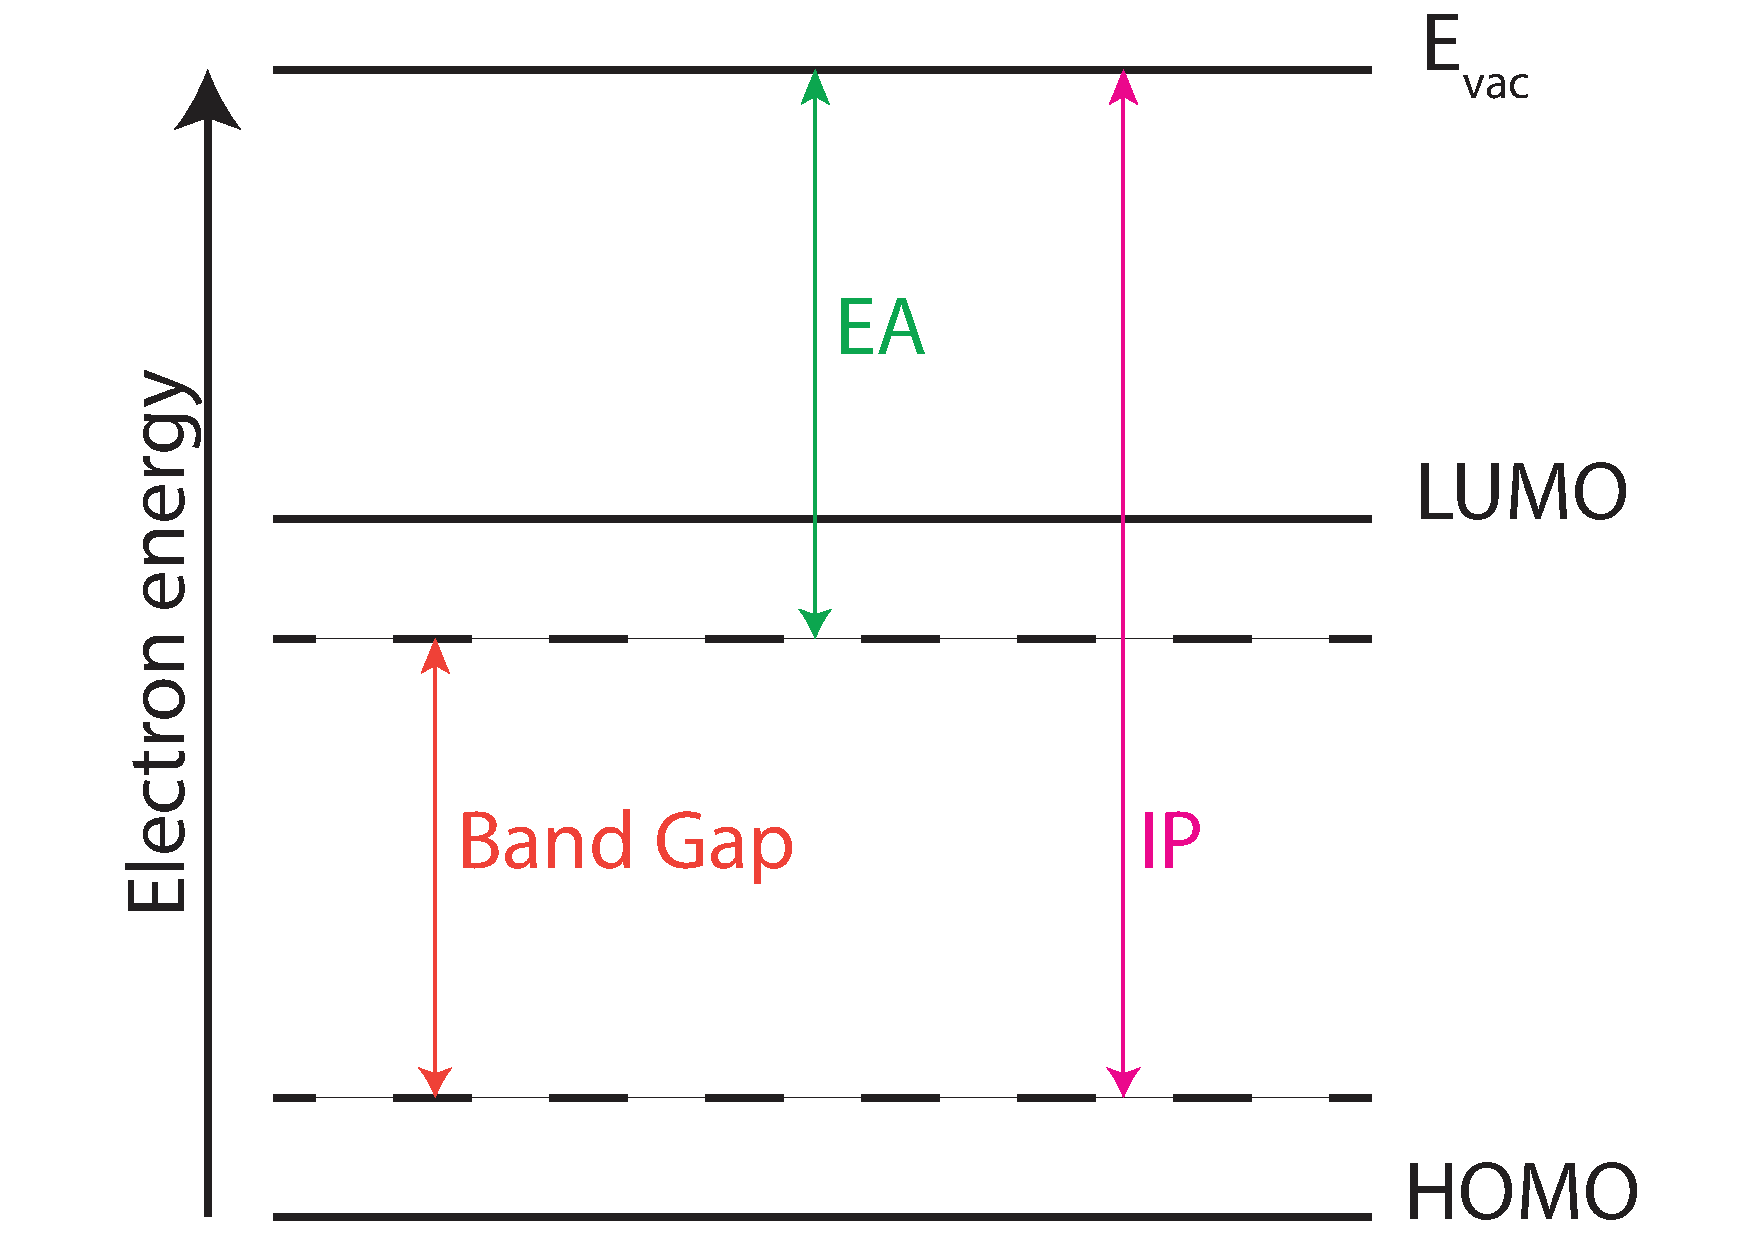
\includegraphics{./images/HOMOLUMO1.pdf}

}

\caption{\label{fig-homo}HOMO-LUMO energy diagram for organic
semiconductors showing the electron affinity (EA), ionization potential
(IP), and the bad gap in relation to the energy needed to reach vacuum}

\end{figure}

\begin{figure*}

\begin{longtable}[]{@{}ccccc@{}}
\caption{\textbf{OLED host, dopant, and charge generation
molecules}}\tabularnewline
\toprule()
Organic molecule & Formula and molecular weight (amu) & HOMO {[}LUMO{]}
& Application & Ref. \\
\midrule()
\endfirsthead
\toprule()
Organic molecule & Formula and molecular weight (amu) & HOMO {[}LUMO{]}
& Application & Ref. \\
\midrule()
\endhead
Alq3 & \(C_{27}H_{18}AlN_3O_3\ 459.43\) & \(-5.7\ [-2.9]\) & Electron
transport and host & (Djurovich et al. 2009; Tao, Yang, and Qin 2011) \\
TPBI & \(C_{45}H_{30}N_6 \ 654.76\) & \(-6.2 \ [-2.7]\) & Electron
transport and exciton blocking & (Tao, Yang, and Qin 2011) \\
NPB & \(C_{44}H_{32}N_2 \ 588.74\) & \(-5.4 \ [-2.3]\) & Hole transport
& (Tao, Yang, and Qin 2011; J. Liu, Zhang, et al. 2015) \\
DPA & \(C_{26}H_{18} \ 330.42\) & \(-5.6 \ [-2.6]\) & Fluorescent and
Host & (J. Liu, Zhang, et al. 2015) \\
TMPYPB & \(C_{39}H_{27}N_3\ 537.65\) & \(-6.7 \ [-2.7]\) & Electron
transport and exciton blocking & (Tao, Yang, and Qin 2011; J. Liu,
Zhang, et al. 2015) \\
mCBP & \(C_{36}H_{24}N_{2} \ 484.6\) & \(-5.6\ [-2.1]\) & Host & (Wong
and Zysman-Colman 2017) \\
TAPC & \(C_{46}H_{46}N_2 \ 626.37\) & \(-5.5 \ [-2.0]\) & Hole transport
& (Tao, Yang, and Qin 2011) \\
Coumarin6 & \(C_{20}H_{18}N_2O_2S \ 350.43\) & \(-5.2\ [-1.7]\) &
Fluorescent and laser dye & (Agrawal et al. 2011) \\
\bottomrule()
\end{longtable}

\end{figure*}

\begin{figure}

{\centering 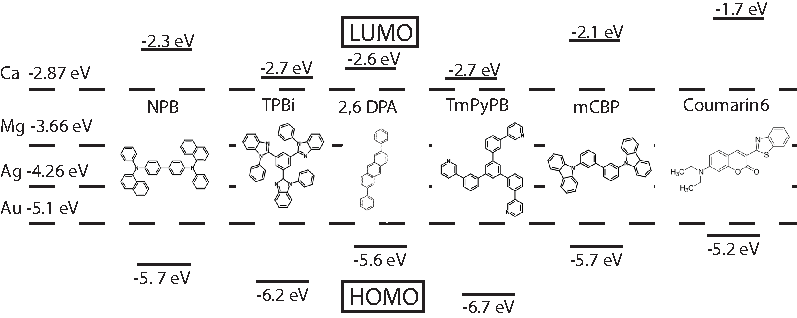
\includegraphics{./images/Struct.pdf}

}

\caption{\label{fig-widestruc}The organic structures of molecules found
in this thesis and their respective HOMO/LUMO levels in relation to
Fermi level of common metals}

\end{figure}

::: A photon can be incident upon the molecule to excite the
\(\pi\)-electron to form an electron-hole pair. This delocalized charge
pair is called an exciton. Excitons are stable at room temperature
because of their large binding energy (\(1 eV\)) compared to its thermal
activation energy (\(k_BT=25 meV\)) (Gärtner 2009). It is then easier to
interpret the optical (and electrical) properties in this exciton
picture. Excitons have many excitonic states, but the lowest is the
ground state \(S_0\). Each excitonic state has many sub-states that
offshoot energetically due to vibrational fluctuations (see
Figure~\ref{fig-absorb}). The bandgap separates the ground state \(S_0\)
and the first excited state \(S_1\). A photon can excite the exciton
from the ground state to a higher vibronic state of a singlet state, and
then subsequently relax to the lowest vibronic state in 1 ps timescale.
Then the lowest vibronic state of the \(S_1\) can decay either
radiatively (emitting light) or nonradiatively to the groundstate with a
lifetime of 1 ns. Because the absorption normally transitions to a
higher vibronic state and then relax to a lower vibronic state, the
emission spectra tends to be redshifted (lower energy) compared to the
absorption spectra. This energy difference between the spectra is
referred to as Stokes shift (Forget and Chénais 2013; Gärtner 2009).
Lasers benefit from Stokes shift because it helps reduce self absorption
losses.

\begin{figure}

{\centering 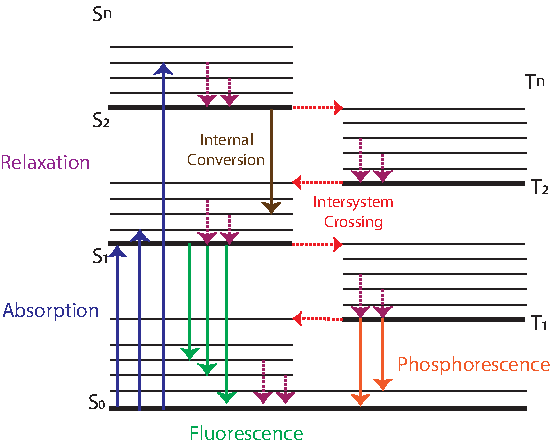
\includegraphics{./images/absorb.pdf}

}

\caption{\label{fig-absorb}Basic transitions within an organic molecule
between the ground state \(S_0\) and the excited singlet \(S_1\),
\(S_2\),\ldots{} \(S_n\) and triplet states \(T_1\), \(T_2\),\ldots{}
\(T_n\), represented in a Jablonski diagram}

\end{figure}

Excitons, after they absorb a photon, transition to the singlet state.
Singlet states can undergo fluorescent decay (emission of light) or
undergo intersystem crossing (ISC) into the triplet state. In typical
fluorescent devices, the lifetime of fluorescent decay is much shorter
than ISC. ISC becomes enhanced in phosphorescent materials because of
their strong spin-orbit coupling. The triplet state \(T_1\) has long
lifetimes of \(\mu s\)-\(ms\), which have subsequent pathways that
include phosphorescent decay or reverse intersystem crossing (RISC).
These pathways are shown in Figure~\ref{fig-absorb}. Triplet
deactivation are dominated by nonradiative decay at room temperature,
hence why triplets are usually called non-emissive states.
Phosphorescent decay can be increased by using heavy metal atoms with
strong spin-orbit coupling.

Opposed to a radiative decay (fluorescence) with a decay rate \(k_r\), a
molecule can decay nonradiatively to the groundstate by internal
conversion (IC). It has a decay rate \(k_{nr}=\tau_{nr}^{-1}\). To avoid
nonradiative decay (NRD), a rigid and planar molecular structure can be
introduced to not have the vibrational coupling of \(S_1\) and \(S_0\)
states, i.e.~the \(S_1\) will not vibrationally transfer its energy to
\(S_0\). Small band gap (long-wavelengths) molecules will suffer from
vibrational coupling -- the effect is labeled the energy gap law.

\hypertarget{electrical-properties-of-organic-semiconductors}{%
\section{Electrical properties of organic
semiconductors}\label{electrical-properties-of-organic-semiconductors}}

This section will be more detailed than the optical
Section~\ref{sec-opti} because this report mainly focuses on
electrically pumped laser diodes and OLEDs. First the basics will be
discussed, followed by charge carriers and their process from injection
to transportation.

\hypertarget{charge-carriers}{%
\subsubsection{Charge carriers}\label{charge-carriers}}

Electrons and holes within an organic semiconductor interact stronger
with the fixed atoms than in inorganic materials (Gärtner 2009). This
stronger interaction causes a new consideration for holes and electrons
-- a quasiparticle called a polaron (Forget and Chénais 2013). The lower
polaronic state is occupied by a single charge, while the upper
polaronic state is occupied with two charges. The LUMO level fills the
lower polaronic state with positive polarons (holes) and the HOMO level
fills the higher polaronic state with negative polarons (electrons). The
polaronic stated cause additional absorption bands, resulting in a new
type of loss: polaron induced absorption.

\hypertarget{charge-transport}{%
\subsubsection{Charge Transport}\label{charge-transport}}

Charge carriers in conjugated polymers are localized to a portion of the
polymer chain, usually called the active unit or chromophore, because of
the lack of long-range translational symmetry (L. Li and Kosina 2010;
Gärtner 2009). Thus the only way for charges to transfer between
neighbouring molecules is via phonon assisted tunnelling, or a
stochastic hopping process. The mobility of this hopping in organic
semiconductors is between \(10^{-8} cm/Vs\) to \(10^{-3} cm^2/Vs\).
Because hopping is highly inefficient, it explains the very low carrier
mobilities in organic semiconductors, contrasted to their inorganic
counterparts (Forget and Chénais 2013). The charge transport of an
organic material is given by its electric conductivity \(\sigma\) that
depends on the density of the charge carriers \(n\), and the charger
carrier mobility \(\mu\), given by \[\sigma = \mu n q\]where \(q\) is
the elementary electron charge (Forget and Chénais 2013). We can see
from this relation that in order to achieve high electrical
conductivity, and thus a high charge transport, the charge carrier
mobility must be high. Further information on charge transport in
organic semiconductors can be found in Refs. (L. Li and Kosina 2010;
Shirota and Kageyama 2007; Coropceanu et al. 2007).

\hypertarget{electron-hole-recombination}{%
\subsubsection{Electron-hole
recombination}\label{electron-hole-recombination}}

Similar to optical properties, because the exciton is stable at room
tempetature, it is best to consider the the charge carrier pair in the
exciton picture. In organic semiconductors, recombining electrons and
holes generate excitons. Light emission is thus the radiative decay of
these excitons. The recombination is governed by Langevin theory (Pope
and Swenberg 1982), such that we get the exciton formation formula
\[e + h \rightarrow
\begin{cases}
    1/4,& S_n^*\rightarrow S_1\\
    3/4,& T_n^*\rightarrow T_1
\end{cases}\] where \(S_n\) and \(T_n\) are the higher-lying singlet and
triplet states respectively (Gärtner 2009). Their lifetime is about 1 ps
because of their ultra fast relaxation to the lowest excited state
\(S_1\) or \(T_1\). Spin statistics (Adachi and Sandanayaka 2020) govern
the 3:1 generation ratio of triplets to singlet excitons, which has been
experimentally determined (Lupton et al. 2005). It is also important to
note that these probabilities occur only when the singlet--triplet gap
is much less than \(k_BT\). Most practical molecules are within this
bound at room temperature; however, if the singlet--triplet gap is much
larger than \(k_BT\), triplets form with nearly \(100\%\) probability
(Jacko, McKenzie, and Powell 2010). In other words, excitons decay to
the ground state via the lowest triplet state if the singlet--triplet
energy gap is larger than \(k_BT\).

The recombination of holes and electrons have a rate that is given by
\[\gamma = \frac{e(\mu_e+\mu_h)n_e(x,t)n_h(x,t)}{\epsilon_r\epsilon_0}\]
where recombination \(\gamma\) is a function of the charge carrier
mobilities \(\mu_e\) and \(\mu_h\), and the electron density
\(n_e(x,t)\) and hole density \(n_h(x,t)\). From this, high exciton
generation needs high mobility materials as well as higher particle
densities. Hole mobility is typically one order of magnitude larger than
the electron mobility -- such a difference means the recombination
\(\gamma\) mainly depends on the higher mobility.

\hypertarget{charge-carrier-injection}{%
\subsubsection{Charge carrier
injection}\label{charge-carrier-injection}}

To pass a current (charges) through an organic semiconductor it has to
be sandwiched between an anode and cathode. The entire structure is
called an organic semiconductor light emitting diode (OLED). Once a
voltage is applied across the electrodes, the electrons and holes
diffuse through the layers. While OLEDs usually have a current density
of a few \(mA/cm^2\), laser diodes require much higher current
densities. The electrons are injected into the LUMO and the holes into
the HOMO to form an exciton. OLEDs will be discussed further in
Section~\ref{sec-OLED}.

\hypertarget{energy-transfer}{%
\subsection{Energy Transfer}\label{energy-transfer}}

Excitons play a pivotal role into how the organic molecule emits light
but their dynamics are not as simple as stationary particles. They can
have their energy transferred across several nanometers, which enables
movement between identical molecules and between a host/guest system.
These energy transfers can enable unique energy pathways to increase the
total light emission. The two main transfers in organic semiconductors
will be discussed next.

\hypertarget{fuxf6rster-resonance-energy-transfer}{%
\subsubsection{Förster resonance energy
transfer}\label{fuxf6rster-resonance-energy-transfer}}

Förster (sometimes called fluorescent) resonance energy transfer (FRET)
is a resonant energy transfer process between two singlet exciton states
of two molecules. It is a resonant process because the excited donor
molecule (\(D^*\)) decays without emission of a photon, and then
transfers the energy to an accepting molecule (A) (see
Figure~\ref{fig-FRET}). FRET is goverend by Fermi's golden rule for
transfer between states, which means they have a transfer rate
\(\Gamma_{DA}\) from a donor (D) to acceptor (A) is
\[\Gamma_{DA} = 4\pi^2|V_{DA}|^2]\delta(E_A-E_M)\] where \(V_{DA}\) is
the matrix element for interaction of the donor and acceptor, who have
energies \(E_D\) and \(E_A\) respectively (Gärtner 2009). The
\(\delta\)-function describes the need for the energies to match, or at
least have spectral overlap of the absorption and emission spectrum.
Even though the energy transfer occurs without the emission of a photon,
we tend to say that typically the spectrum of the donor \(g_A(E)\)
overlaps with the \emph{absorption} spectrum of the acceptor \(g_D(E)\).
The long-range dipole-dopole interactions between D and A cause the
pairing of spectrum overlap. This coupling influences the rate of energy
transfer, as well as the quantum yield of the donor, the relative
orientation of D and A transition dipoles, and the distance between the
molecules. Integrating over the spectral overlap and evaluating the
interaction matrix elements provides the Förster formula which provides
the total transfer rate \(k_{DA}\)
\[k_{DA} = 8.8\times10^{17} \frac{\kappa^2}{n^4\tau_Dr^6}\int g_A(E)g_D(E)dE\]
which then can be written as
\[k_{DA}(r) = \frac{1}{\tau_D}\left(\frac{R_0}{r}\right)^6\] where
\(\tau_D\) is the decay time of the donor in the absence of the
acceptor, \(\kappa\) is the relative orientation of the dipoles, \(R_0\)
is the Förster distance (typically a few nanometers (Lakowicz 2006)),
and \(r\) is the D-to-A distance. Clearly, FRET is an extremely distance
dependent process (\(k_{FRET}\propto r^{-6}\)). FRET usually occurs at
distances of 20 to 90 Å, typical distances of proteins or membrane
thickness (Lakowicz 2006). The transitions must be allowed, so that is
why this process only works for singlet excitons.

FRET is mainly seen in a host/guest system, where in order to get
singlets from the host to guest, we utilise FRET to transfer singlets on
the host to the guest. FRET governs some of the bimolecular annihilation
processes that are important in organic semiconductors. The key takeaway
from this information is that this process is distance dependent, with a
\(50\%\) efficiency at \(r=R_0\) calculated from the efficiency \(\rho\)
of the energy transfer (Forget and Chénais 2013)
\[\rho = \frac{1}{1+\left(\frac{r}{R_0}\right)^6}\]

\begin{figure}

{\centering 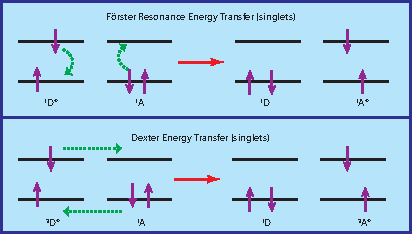
\includegraphics{./images/FRET.pdf}

}

\caption{\label{fig-FRET}Förster resonance energy transfer is a
dipole-dipole interaction, where in the absence of a photon, the Donor D
releases energy that is reabsorbed by the acceptor A. The must be
overlap between emission spectrum and absorption spectrum for the
transfer to happen. Dexter energy transfer has simultaneous exchange of
electrons and holes, such that an exciton is transferred between D and
A. Singlets are displayed here, but Dexter energy transfer does work for
triplets too.}

\end{figure}

\hypertarget{dexter-energy-transfer}{%
\subsubsection{Dexter energy transfer}\label{dexter-energy-transfer}}

DET is one of the mechanisms of short-range quenching, and like the name
suggest the molecules need to be close. So close in fact that the D
molecule and quencher Q must have their electronic clouds overlap. DET
describes an exchange of electrons from the LUMO of the donor to the
LUMO of the acceptor. Similarly the hole is transferred the other way in
the HOMO. Such that the net transfer in a host/guest system is an
exciton moving between the D and A (Dexter 1953). The difference between
DET and Fret can be found in in Figure~\ref{fig-FRET}. The rate of DET
\(k_{DET}\) is \[k_{DET} = \hbar P^2Je^\frac{-2r}{L}\] where r is
distance between D and A, \(J\) is the spectral overlap, and the other
variables, P and L, are constants that are hard to quantify (Dexter
1953). DET occurs only across distances between \(0.5\)-\(2\) nm,
compared to the \(2\)-\(10\) nm of FRET.

\hypertarget{losses-in-organic-semiconductors}{%
\section{Losses in organic
semiconductors}\label{losses-in-organic-semiconductors}}

The current densities needed to achieve organic laser diodes are
estimated to be at least \(1 kA/cm^2\) (Adachi and Sandanayaka 2020). In
organic semiconductors, to obtain this threshold means that the particle
densities must be around \(10^{19}/cm^3\) and electric fields of up to
\(10^7 V/cm\) are needed -- this is considering the low mobilities of
organic semiconductors \(10^{-8}-10^{-3}cm^2/Vs\) (Gärtner 2009). Thus
the populations of excitons will need to be extremely high -- a perfect
environment for increased bimolecular annihilation processes. Here, a
description of these process will be described.

Bimolecular annihilation processes occur between particles within the
organic semiconductor, such as charge carriers and excitons. Most of
these processes quench the emissive singlet excitons (see
Figure~\ref{fig-biomoc}). Hence, these processes are important to
realising efficient light emission. The diagram indicates the particle
species by the circles, and which population they are quenching by the
direction of the arrows. \protect\hyperlink{tab:bimoc}{Table 1.2} shows
the processes in terms of donor (D) and acceptor (A).

\begin{figure}

{\centering 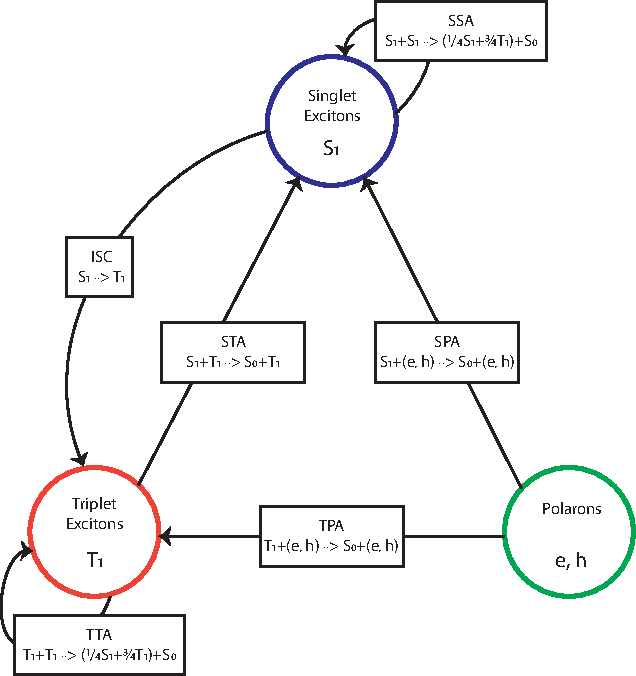
\includegraphics{./images/bimoc.pdf}

}

\caption{\label{fig-biomoc}The bimolecular annihilation process are
displayed in relation to singlets {S1}, triplets {T1}, and polarons e
and h. Notably, most of these processes quench the emissive singlet
excitons.}

\end{figure}

\hypertarget{tab:bimoc}{}
\begin{longtable}[]{@{}clcllllc@{}}
\caption{Bimolecular processes in organic materials. The system has a
donor D with an excited state density \(D^*\) and an acceptor A with
excited state density \(A^*\). A quencher Q is some foreign element such
as dissolved oxygen or water. Table from (Forget and Chénais
2013).}\tabularnewline
\toprule()
Excited molecule & & Other element & & & & & Process \\
\midrule()
\endfirsthead
\toprule()
Excited molecule & & Other element & & & & & Process \\
\midrule()
\endhead
\(D^*\) & + & \(D\) & \(\rightarrow\) & \(D\) & + & \(D^*\) &
Diffusion \\
\(D^*\) & + & \(D^*\) & \(\rightarrow\) & \(D\) & + & \(D^*\) &
SSA/TTA \\
\(D^*\) & + & \(Q\) & \(\rightarrow\) & \(D\) & & & Quenching \\
\(D^*\) & + & \(A\) & \(\rightarrow\) & \(D\) & + & \(A^*\) & FRET \\
\bottomrule()
\end{longtable}

\hypertarget{singlet-singlet-annihilation-ssa}{%
\subsubsection{Singlet-singlet annihilation
(SSA)}\label{singlet-singlet-annihilation-ssa}}

The emissive excited state donor \(D^*\) moloecule can be quenched by
the identical molecule, which when represented in the singlet-singlet
process (\(D^*=S_1\)) is \[S_1 + S_1 \rightarrow S_n + S_0\] where
\(S_1\) is the excited singlet state and \(S_0\) is the ground state
(Thompson et al. 2014; Nakanotani, Sasabe, and Adachi 2005). One
molecule falls to the ground state, the other gets excited to a higher
singlet state \(S_n\) that has a chance to decay either to the singlet
state or the triplet state. The rate of SSA \(k_{SSA}\) in terms of the
\(S_1\) population is given by
\[\frac{dS_1}{dt} = -(2-\zeta)k_{SSA}S_1^2\] where \(\zeta\) factor is
because not all excited states \(S_n\) are returned to the \(S_1\)
state. The spin conservation is governed by spin statistics (Lupton et
al. 2005), usually \(\zeta=0.25\) (Thompson et al. 2014). \(k_{ss}\) is
usually on the order of \(10^{-9} cm^3/s\). To measure this rate
constant \(k_{SSA}\) transient photoluminescence measurements can be
done (Sokolik et al. 1996), which involves a pulse measurement to a
width less than the lifetime of radiative singlet decay. Naturally, when
the population of singlets are low, the rate of SSA becomes negligible.

\hypertarget{exciton-polaron-annihilation}{%
\subsubsection{Exciton-polaron
annihilation}\label{exciton-polaron-annihilation}}

Both singlet-polaron annihilation (SPA) and triplet-polaron annihilation
occur under electrical injection because of the high lifetimes of
polarons. The basic concept is the excitons transfer their energy by
deactivation to the polaron via the process
\[S_1 / T_1 + (e,h) \rightarrow S_0 + (e,h)\] where the rate of
\(k_{SPA}\) can be different for hole or electron quenching. At low
current densities, SPA is negligible, but starts becoming a serious
issue the more current injected.

\hypertarget{singlet-triplet-annihilation}{%
\subsubsection{Singlet-Triplet
Annihilation}\label{singlet-triplet-annihilation}}

If the \(S_1\) and the \(T_1\) state share overlap, the singlet and
triplets can interact causing an excitation to a higher triplet state
\(T_n\) and a nonradiative decay to the ground state. The process is
\[S_1 + T_1 \rightarrow S_0 + T_n\] For non-TADF materials, where
reverse intersystem crossing (RISC) is unlikely, the excited state
\(T_n\) will relax back to the long-lived \(T_1\) and then subsequently
non-radiatively decay back the ground state. The rate equation for STA
is \[\frac{dS_1}{dt} = -k_{STA}S_1T_1\] where \(k_{STA}\) is usually on
the order of \(10^{-9} cm^3/s\). This process is a FRET type transfer,
and especially dominate in conjugated polymers(List et al. 2002) because
the triplets accumulate in the device due to their long lifetimes.

\hypertarget{intersystem-crossing-isc}{%
\subsubsection{Intersystem Crossing
(ISC)}\label{intersystem-crossing-isc}}

For every excited singlet state, a triplet state lies lower in energy by
an amount \(\Delta E_{ST}\) that is often referred to as the
singlet-triplet splitting. While not pertinent to understand why this is
the case, the extremely simplified explanation is that Pauli exclusion
principle forces the spatial factor of the singlet wave function to be
symmetric and anti-symmetric for the triplet wave function. This
symmetry/antisymmetry causes the mean potential energy of the electrons
to be higher for singlets than triplets with the same quantum numbers n
and m. To read more in detail see Ref. (Stuke 1992). This relationships
means we get overlap with the wave functions that scales exponentially
with \(\Delta E_{ST}\). Thus a nearly spontaneous transfer from the
\(S_1\) population to the lower \(T_1\) state becomes possible, which is
called intersystem crossing (ISC). The pathway can be seen in
Figure~\ref{fig-ISC}. The ISC rate equation \(k_{ISC}\) can be formed:
\[\frac{dT_1}{dt} = k_{ISC}S_1\] Fluourscent emitters have ISC rates on
the order of hundreds of nanoseconds (\(k_{ISC} ~ 10^7s^{-1}\) (Forget
and Chénais 2013), with a timescale of \(\tau_{ISC} = 1/k_{ISC}\). This
rate depends strongly on the spin-orbit coupling, as well as the
vibrational overlap of the wavefunctions (Stuke 1992).Reverse
intersystem crossing (RISC) is the same process in reverse, but it is
usually only seen in thermally activated delayed fluorescent materials
where the \(E_{ST}\) is small.

\begin{figure}

{\centering 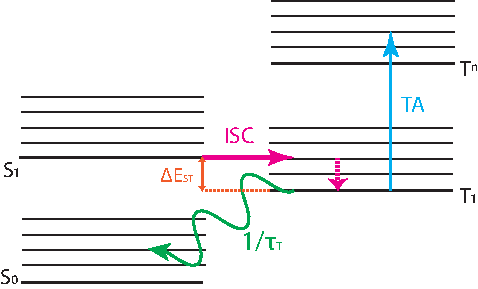
\includegraphics{./images/ISC.pdf}

}

\caption{\label{fig-ISC}Intersystem crossing (ISC) displayed in a
Jablonski diagram, along with Triplet Absoprtion (TA), and
singlet-triplling splitting {ΔEST} in a conjugated system.}

\end{figure}

\hypertarget{triplet-triplet-annihilation-tta}{%
\subsubsection{Triplet-Triplet Annihilation
(TTA)}\label{triplet-triplet-annihilation-tta}}

Organic semiconductors under electrical excitation generate triplets at
a \(75\%\) chance to \(25\%\) singlets. This means that in these
molecules triplet-triplet annihilation plays a major role in the triplet
dynamics, especially because triplets are long-lived. The two triplet
excitons interact (annihilate) causing a transfer of energy from the
first exciton to the second. The excited exciton goes to a higher lying
state, which then relaxes so a singlet, triplet, or quintlet state.
Although this bimolecular process can be considered a loss, it can also
lead to gain via the generation of singlets out of triplets. Hence the
focal point of this thesis is "Can TTA be utilised to manage the triplet
states to increase the efficiency of emission such that organic laser
diodes can be realised?". Triplet-triplet annihilation will be discussed
in further in Section \protect\hyperlink{sec:type}{1.5.0.3}.

\hypertarget{induced-absorption}{%
\subsubsection{Induced absorption}\label{induced-absorption}}

Photons incident upon the conjugated molecule can be quenched by
polarons and triplets because of the additional absorption bands. The
triplets and polarons care excited to a higher lying state and then
relax back to the original position. These losses only substantially
affect laser diodes, so it will not be discussed any further. For more
information, see Ref. (C.-L. Lee, Yang, and Greenham 2007) for triplet
absorption (TA) and Ref. (Chakaroun et al. 2011) for polaron absorption
(PA).

\hypertarget{sec-OLED}{%
\section{Organic light emitting diodes (OLEDs)}\label{sec-OLED}}

This thesis has the goal of achieving organic laser diodes; but in order
to get there, OLEDs are the more cost efficient and easier method of
analysing the emissive layer. This thesis first aims to determine the
triplet-triplet annihilation property of an emissive layer, followed up
by analysing the success of doping a TTA-exhibiting host with a
efficient lasing guest. To do this, fabrication of OLEDs will be able to
test the electrical characteristics and performances of these materials.

\hypertarget{device-structure}{%
\subsubsection{Device structure}\label{device-structure}}

To pass a current through an organic semiconductor, it has to be
sandwiched between an anode and cathode, where we call the entire
structure an OLED device. Once a voltage is applied across the
electrodes, the electrons and holes diffuse through the layers. The
exciton forms on the host, but if a dopant is present within the
emissive layer, the exciton transfers to the guest via either Förster
resonance energy transfer or by Dexter energy transfer (V. Duarte F. J.
2018; Forget and Chénais 2013). To avoid non-radiative losses (via
heat), as shown in Figure~\ref{fig-homo} the host IP is usually larger
than the guest HOMO. This enables a minimal barrier for the transferring
electron to overcome. Similarly, the cathodes -- typically indium tin
oxide (ITO) as the anode and aluminium doped with calcium as the cathode
-- operate better if their work function align with the IP and EA of the
organic layers. Matching the energy levels of each layer within an OLED
is crucial to efficient device performance. Discussion of the energy
levels concerned with this report's devices can be found in their
relevant section.\\

\begin{figure}

\begin{minipage}[t]{0.50\linewidth}

{\centering 

\raisebox{-\height}{

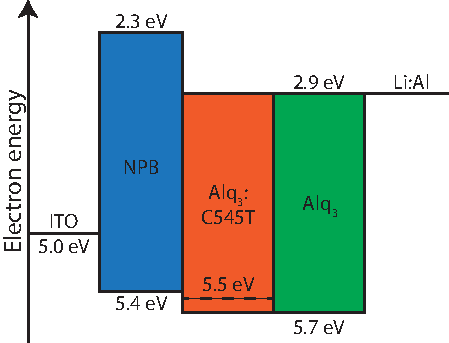
\includegraphics{./images/Asset 3 (1).pdf}

}

}

\subcaption{\label{fig-wideA}}
\end{minipage}%
%
\begin{minipage}[t]{0.50\linewidth}

{\centering 

\raisebox{-\height}{

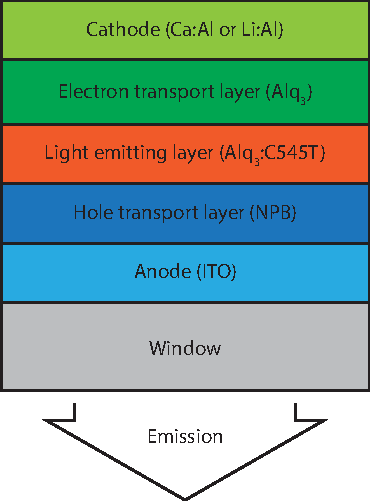
\includegraphics{images/Asset 2 (1).pdf}

}

}

\subcaption{\label{fig-wideB}}
\end{minipage}%

\caption{\label{fig-elephants}Figure (a) is an example of a simple OLED
device with its energy level diagram (b). Holes are injected from the
anode into the hole transport layer (HTL) such that the holes then have
an easier time entering the emissive layer. Similar to the anode,
electrons enter from the cathode into the electron transport layer
(ETL). Electrons and holes recombine in the light emitting layer (EML),
forming an exciton that has four possible permutations: three triplet
states each with a total spin of 1, and one singlet state with a total
spin of zero.}

\end{figure}

Modern day OLED architectures consist of as many as five or more organic
layers (see Figure~\ref{fig-wideA}), where each layer helps improve the
luminescence efficiency, reduce operational voltage, and improve
operational stability (V. Duarte F. J. 2018; C. W. Tang and VanSlyke
1987; Adachi et al. 1988). The purpose of these layers were to give fine
control over the charge injection, charge transport, electron-hole pair
(exciton) diffusion, and photon emission. These improvements led to OLED
devices reaching the threshold efficiencies, and some now consider them
better than inorganic LEDs.

\hypertarget{performance-characteristics}{%
\subsubsection{Performance
characteristics}\label{performance-characteristics}}

It is extremely useful to define the efficiency of emitted fluorescence
photons versus the number of inputted photons or polarons (depending on
photoluminescence or electroluminescence). Such a ratio, called the
photo/electroluminescence quantum yield \(\phi_F(0<\phi_F<1)\), enables
meaningful discussion about the efficiency of the device and where the
losses come from. It is defined as
\[\phi_F = \frac{k_r}{k_r+k_{nr}+k_{ISC}}=\frac{\tau_nr}{\tau_{rad}+\tau_{nr}+\tau_{ISC}}=\frac{\tau_F}{\tau_{rad}}\]
where \(\tau_F\) is the fluorescence lifetime (Forget and Chénais 2013),
a measure of the singlet state's effective lifetime. The total decay
rate \(k\) is the sum of the radiative decay \(k_r\) and nonradiative
decay \(k_{nr}\). The total decay rate follows an exponential function,
which can be fitted to the time resolved luminescence to estimate the
value via \[I(t) = I_0e^{-kt}\] where \(I_0\) and I(t) is the initial
and time response luminescence intensities, respectively. The total
efficiency of a device is more than just the fluorescence quantum yield.
This external quantum efficiency (EQE) is the total performance
efficiency of the device that is given by
\[\phi_{EQE} = \gamma \phi_{spin}\phi_F\eta_{out}\] where \(\gamma\) is
a factor describing how often charges recombine in the emissive layer
(usually \(\gamma \approx 1\)), \(\phi_{spin}\) is the singlet-triplet
spin probability factor (in fluorescence \(\phi_{spin} ~ 0.25\)), and
\(\eta_{out}\) is a factor describing the percentage of light escaping
the device (usually \(\phi_{out} ~ 20-25\%\)). \(\gamma\) and
\(\eta_{out}\) are altered via the device architecture, while \(\phi_F\)
and \(\phi_{spin}\) are altered via the emissive layer. To put it into
context for this report, one focus is to choose the right emissive layer
to obtain high \(\phi_F\) and \(\phi_{spin}\) and by proxy a high EQE.
In this thesis, \(\phi_{spin}\) will be increased by utilising TTA, the
process that generates extra singlet excitons from the triplets.
\(\phi_F\) is low for TTA materials, so hence why it will be doped with
a more efficient lasing material.

OLEDs also need to consider operational lifetime, a key attribute that
is directly proportional to the degradation of the devices due to losses
such as localized heating, material decomposition, and Coulombic
degradation (Aziz et al. 1999; T.-H. Liu, Iou, and Chen 2003; K. K. Lin
et al. 2001; Meerheim et al. 2006; Jiang et al. 2007; Cester et al.
2010). If the luminance efficiency is increased and thus reduces the
current needed to achieve a target brightness, the operational lifetime
is increased. This is why it is so important to try and reduce the
current input, especially for electrically pumped lasers. A typical OLED
display operates at around \(0.01 A cm^{-2}\); a typical inorganic
semiconductor laser diode operates at a current density of
\(1000 A cm^{-2}\) (I. D. W. Samuel and Turnbull 2007). Hence decreasing
the current-density threshold by making the device more efficient is
necessary to achieving lasing. This is part of the motivation for this
thesis.

\hypertarget{sec-type}{%
\subsubsection{Types of emissive layers}\label{sec-type}}

Any light emitted from electrical injected we label as
electroluminescence (photoluminescence for optically pumped). To compare
all the different ways emissive layers electroluminesce, the layers are
labelled depending on their emission pathway. Light emission via singlet
exciton decay is labelled as fluorescence. Because fluorescent materials
can only emit photons from the singlet excited state (V. Duarte F. J.
2018; Forget and Chénais 2013; Adachi and Sandanayaka 2020), their
internal quantum efficiency (IQE) is limited to \(25\%\). We do not see
emission from the triplet excites states because the nonradiative decay
out-competes radiative decay at room temperature (Adachi and Sandanayaka
2020). At low temperatures, triplet-state emission is possible, but is
impractical. Up until 1997, most light emitting devices used fluorescent
materials.

Organic phosphorescent dopants were discovered to be able to emit
photons from the decay of triplet excited states due to strong
spin-orbit coupling, which led to high IQEs. They also have fast rates
of singlet-triplet intersystem crossing (ISC). This meant that these
phosphorescent materials could be used as a guest to extract the
triplets and singlet excited states via Dexter energy transfer from the
host. IQEs of up to \(100\%\) were achievable (Adachi et al. 2001; Baldo
et al. 1999). Phosphorescent materials struggle at achieving operational
stability compared to fluorescent materials, especially in the blue
emission regime (Zhang, Lee, and Forrest 2014).

Thermally activated delayed fluorescence (TADF) emitters offer an
alternative way to harness the triplets than phosphorescent materials.
In TADF materials, the splitting \(\Delta E_{ST}\) between the singlet
and triplet excited-states enables the triplet exciton to transfer to
the singlet state via an efficient reverse intersystem crossing (RISC)
process. The process needs thermal energy to transfer between energy
states; so typical TADF materials have a splitting of less than
\(0.5 eV\) such that the thermal energy from room temperature suffices.
Thus in a TADF emitter, the initial singlet excitons decay radiatively
with a prompt emission (nanosecond timescale), which is then followed by
a delayed emission from the triplet-to-singlet RISC decay (microsecond
to millisecond timescale).

Figure~\ref{fig-emitters} compares the emission mechanism in
fluorescent, phosphorescent, and TADF emitters in a Jablonski diagram.
Understanding these dynamics of exciton population and emission pathways
is crucial to obtaining an efficient device. In terms of organic lasing,
the long decay lifetimes of triplet states are the biggest disadvantage
for phosphorescence, along with its scarcity and expensiveness of its
materials. The TADF pathway has slow reverse intersystem crossing, which
means that any realisation of lasing through this pathway will be
unstable because of the slow singlet formation. On the other hand,
fluorescent emitters have short excited-state lifetimes as well as
comparatively higher radiative rates. The issue of course with
fluorescent emitters is their IQE of \(25\%\).

\begin{figure}

{\centering 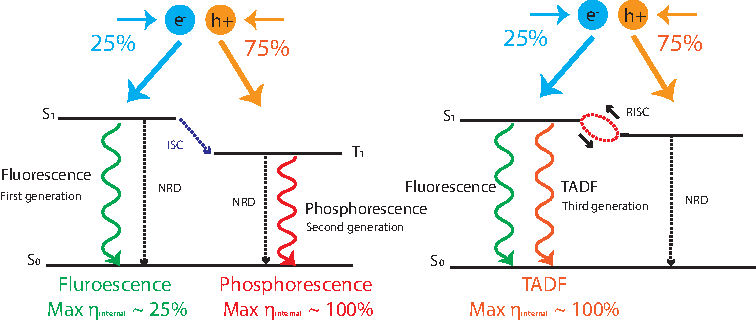
\includegraphics{./images/emitters.pdf}

}

\caption{\label{fig-emitters}The decay mechanisms for singlet and
triplet excitons within fluorescent, phosphorescent, and TADF emitters
in a Jablonksi diagram. As well as the nonradiative decay (NRD) pathway
in all emitters. The diagram features the lowest vibrational level of
the singlet states {S0} (ground state) as well as the first singlet {S1}
and triplet {T1} excited state. Intersystem Crossing (ISC) and Reverse
Intersystem Crossing (RISC) occur between {S1} and {T1}. It also
features the recombination of holes and electrons to form the exciton
quasi-particle and their subsequent exciton formation probability:
{75\%} to triplets and {25\%} to singlets}

\end{figure}

\hypertarget{triplet-triplet-upconversion}{%
\subsubsection{Triplet-triplet
Upconversion}\label{triplet-triplet-upconversion}}

This now enables the introduction of the pathway considered in this
thesis: triplet-triplet upconversion (TTU). Similar to TADF materials,
this pathway has a prompt component and a delayed component. The prompt
emission comes from the direct singlet exciton, while the delayed
emission comes after two triplets annihilate together (via
triplet-triplet annihilation, TTA) and produce a singlet that then
radiatively decays. Triplet-triplet upconversion-based OLEDs have
realised external quantum efficiencies of \(10\%\) as opposed to the
theoretical limit of fluorescence-based OLEDs of \(5\%\).

\begin{figure}

{\centering 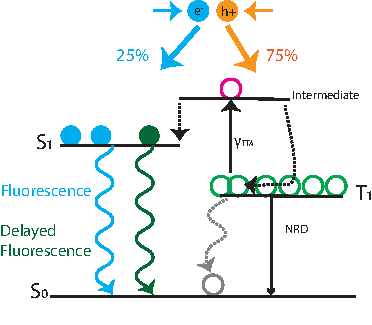
\includegraphics{./images/TTUTTA.pdf}

}

\caption{\label{fig-TTUTTA}The life of an exciton from formation (charge
recombination) to decay via different pathways. Triplet-triplet
annihilation (TTA) with rate constant {γTTA} involves one triplet
non-radiatively decaying to the ground state, and the other being
promoted to an intermediate state. The intermediate state then generates
1/4 singlets and 3/4 triplets, with the Triplets being able to be
recycled.}

\end{figure}

Triplet-triplet annihilation has two colliding triplet states leading to
an intermediate state with twice the energy of the \(T_1\) state. The
intermediate states can then lead to one singlet state, three triplet
states, and five quintet states (Bodo H. Wallikewitz et al. 2012). This
quintet state can be formed due to conservation of total spin angular
momentum, but typically has much higher energy than the two triplet
states at room temperature (Köhler and Bässler 2009; Pope and Swenberg
1982; Zhang and Forrest 2012); so the pathways for the intermediate
state are the higher-lying triplet \(T_n\) state or to a singlet state
\(S_1\) (see Appendix \protect\hyperlink{apen:A}{{[}apen:A{]}}). Writing
it mathematically, the pathways are (Bodo H. Wallikewitz et al. 2012;
Zhang and Forrest 2012; Pope and Swenberg 1982) \[\label{eq:1} 
    T_1 + T_1 \rightarrow T_n + S_0 \rightarrow T_1+S_0\] or
\[\label{eq:2}
    T_1 + T_1 \rightarrow S_1 + S_0\] The generated triplets from the
triplet pathway can be recycled back into further TTA. So assuming no
other decay channels for triplets, the maximum fraction of singlets
\(f_{singlets}\) from this series of TTA is
\[f_{singlets} = \frac{f}{2} \sum_{n=0}^{n=\infty} \left(\frac{1-f}{2} \right)^n = f\frac{1-f}{1+f}\]
where \(f\) is the fraction of \(S_1\) singlets being formed from one
TTA event (Bodo H. Wallikewitz et al. 2012). If \(f=25\%\),
\(f_{singlets}=15\%\). In some new anthracene derivatives, two triplet
states have less energy than the higher lying \(T_n\) state. This means
the triplet pathway is unreachable and only the singlet pathway can be
accessed. In this scenario, \(f=50\), so the maximum singlet generation
can be \(S_{25\%}+(T_{75\%}\times TTA_{50\%} = 62.5\%\). This leads to a
maximum EQE of \(12.5\%\), but this pathway is restricted to a few
materials (Ieuji, Goushi, and Adachi 2019).

The rate constant of TTA \(\gamma_{TTA}\) can be paired with \(f\) to
create the rate constants of each pathway \(f\gamma_{TTA}\) and
\((1-f)\gamma{TTA}\). To develop full singlet and triplet density
dynamics, singlet-triplet annihilation (STA) needs to be included in our
model (Zhang and Forrest 2012). STA has the pathway (Pope and Swenberg
1982) \[\label{eq:3} 
    T + S \rightarrow T + S_0\] with the rate constant \(k_{ST}\). The
full dynamics are therefore
\[\frac{dS}{dt} = \gamma(J) \frac{J}{4ed} - (k_s+k_{s.nr}+k_{ISC}S - k_{ST}ST + f\gamma_{TTA}T^2\]
and
\[\frac{dT}{dt} = \gamma(J) \frac{3J}{4ed} - k_{T,nr}T - k_{ISC}S - (1-f)\gamma_{TTA}T^2\]
where TTU has a rate \(\gamma_{TTU}=f\gamma_{TTA}T^2\) (process
(\protect\hyperlink{eq:1}{{[}eq:1{]}})), process
(\protect\hyperlink{eq:2}{{[}eq:2{]}}) has a rate of
\((1-f)\gamma_{TTA}T^2\), process (\protect\hyperlink{eq:3}{{[}eq:3{]}})
has a rate \(k_{ST}ST\), \(\gamma(J)\) is the charge balance factor
(Giebink and Forrest 2008; Ruhstaller et al. 2001), \(e\) is the
electron charge, \(d\) is the emissive layer thickness, and \(k_s\) and
\(k_T\) are the singlet and triplet natural decay rates. These dynamic
equations can be solved in two limiting stead-state conditions (Bodo H.
Wallikewitz et al. 2012; Qiao et al. 2017; Monguzzi et al. 2008). TTA is
distance-dependent between the neighbouring triplets in solid films,
such that at low current density when minimal triplet exciton population
the mini-triplet decay dominates over the bimolecular triplet
annihilation (\(k{T,nr}T\gg \gamma_{TTU}T^2\)). Setting
\(\gamma(J)\frac{J}{4edk_{T,nr}} \equiv T_{G}\), the triplet population
is \(T = \frac{T_G}{k_{T,nr}}\) such that the singlet population from
TTU in a neat film is \[S = \frac{\gamma_{TTU}}{k_{T,nr}+k_S}T^2\] such
that the luminance L is proportional to current density by
\[L \propto J^2\] In steady state, the EQE can be calculated via
\(EQE(J) = \eta_{out}\phi_{F} \frac{k_sS(J)}{J/(ed)}\), such that at low
current density the EQE is proportional to current density by
\[EQE \propto J\]

At increasing current density, the triplet excitons become abundant and
the bimolecular process dominates the dynamics
(\(k{T,nr}T\ll \gamma_{TTU}T^2\)). In this regime, the \(L\propto J\)
and the EQE becomes insensitive to current, meaning the usual EQE
roll-off would occur. The quadratic dependence on J at low current
densities transitions to the a linear dependence above the critical
triplet density \(T{transition}\>(k_{TTU}\tau)^-1\) (Engmann et al.
2019) (see Figure~\ref{fig-loglogTTU})

\begin{figure}

{\centering 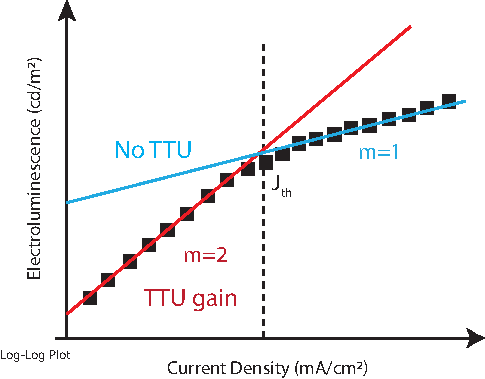
\includegraphics{./images/LoglogTTU.pdf}

}

\caption{\label{fig-loglogTTU}The two regimes of triplet-triplet
annihilation upconversion at low and high current densities. The
transition point {Jth} happens at the critical triplet density
{Ttransition~(kTTUτ)−1}. The graph is a log-log plot.}

\end{figure}

\hypertarget{measurement-of-oled-performance}{%
\subsection{Measurement of OLED
performance}\label{measurement-of-oled-performance}}

To analyse OLEDs performance, such as efficiency, there are numerous
performance characteristics that can be assessed. To record measurements
for an OLED, we can apply a voltage in direct current (DC) operation or
alternating current (AC) via a pulse. The main measurement variables are
voltage (V), current density (\(mA/cm^2\)), and luminance/brightness
(\(cd/m^2\)), with the external quantum efficiency (EQE) needing to be
calculated from these measurements.

\hypertarget{dc-measurements}{%
\subsubsection{DC measurements}\label{dc-measurements}}

In DC measurements, typically measurements of the main three variables
are done over a range of voltages to construct a current
density-voltage-luminance, or J-V-L, graph. In training, I created an
OLED with Super Yellow, poly(phenylenevinylene), as the emissive layer.
Its J-V-L graph shows the natural increase in current density as voltage
is increased -- luminance follows suit too. For the external quantum
efficiency, there usually is a peak EQE for a certain current density.
This is after current density is able to produce sufficient excitons but
before losses start settling in. In this case, STA and polaron quenching
dominate and cause the typical EQE roll off.

\begin{figure}

{\centering 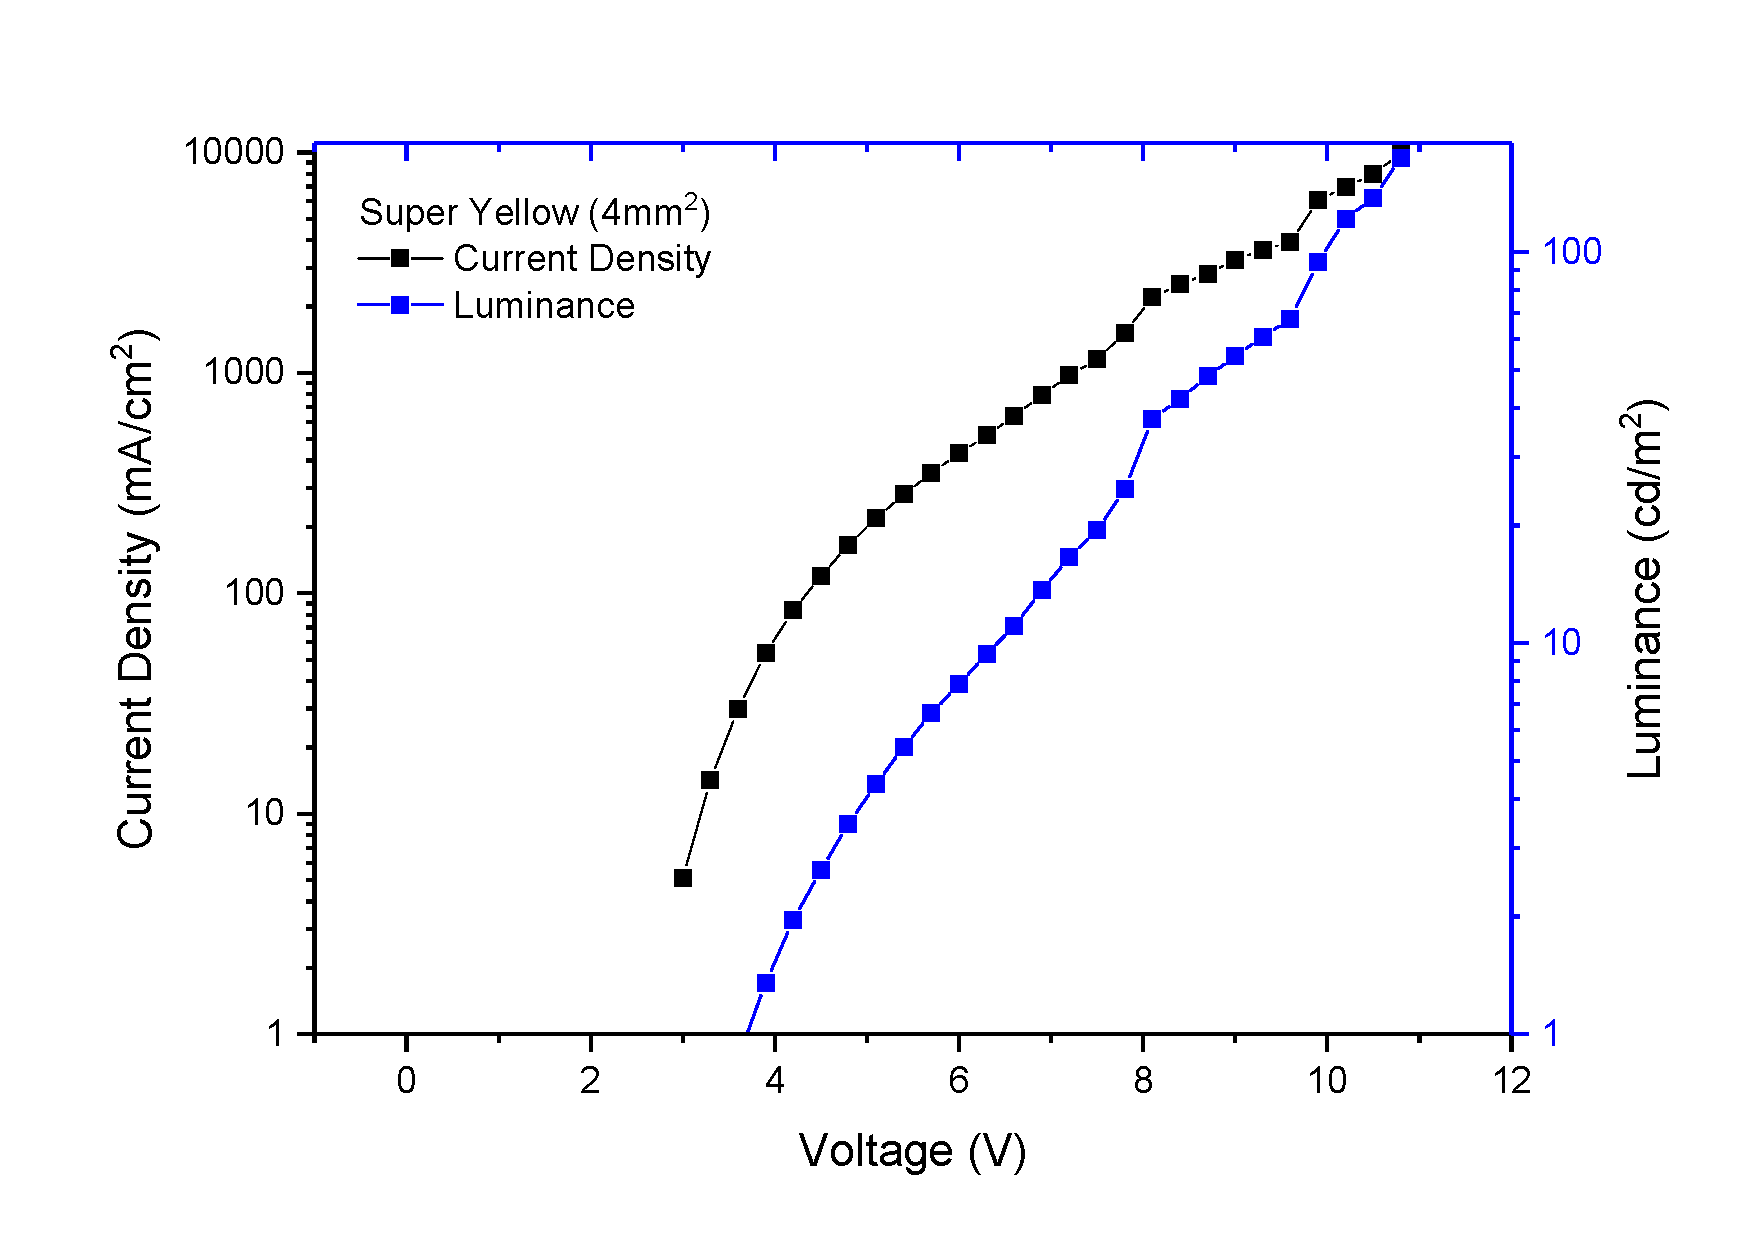
\includegraphics{./images/JVLSY.pdf}

}

\caption{\label{fig-perfo}Performance characteristics for two common
poly(phenylenevinylene) (Super Yellow) devices {[}ITO (100nm)/PEDOT
(30nm)/Super Yellow (70nm)/Calcium (5nm)/Aluminium (60nm){]} that was
made as part of training. a) Typical current density-luminance-voltage
(J-V-L) graph. b) EQE as a function of current density.}

\end{figure}

\hypertarget{pulse-measurements}{%
\subsubsection{Pulse Measurements}\label{pulse-measurements}}

At high current densities, OLEDs experience degradation due to Joule
heating, an effect that causes dark spots on the emitting pixel area of
the OLED. Under DC measurement, Joule heating is amplified. So it
becomes essential to not only use short voltage pulse to one avoid Joule
heating, but also to observe transient electroluminescence. This is
useful because triplet excitons, because they are long-lived, can be
reduced under pulse regime. This leads to reduction in induced
absoprtion losses. In other words, a pulse measurement can achieve a
high singlet population before the triplet excitons approach a
steady-stage. The rates of bimolecular process, as well as decay rates,
can be analysed and calculated via the transient pulse
electroluminescence. No calculations are done in this thesis, but
inclusion of this sets the foundation for the next step.

\hypertarget{organic-semiconductor-lasers}{%
\subsection{Organic semiconductor
lasers}\label{organic-semiconductor-lasers}}

Despite this thesis not containing any fabrication of lasers, it is
still important to discuss what a laser is and how organic
semiconductors can achieve lasing. Lasing was first achieved using ruby
crystals (Maiman 1960), with organic molecules following close after
with optically pumped lasers (Soffer and McFarland 1967; Lemmer et al.
1999). It was not until 1996 that the first organic semiconductor
solid-state laser was developed (Hide et al. 1996), which was the first
step towards reaching organic semiconductor lasers (OSL) that are able
to display the entire visible spectrum. OSLs are even at the stage of
demonstrating lasing while on flexible substrates (Kallinger et al.
1998) and low-threshold operation (Vasdekis et al. 2006), but no stable
electrically pumped lasers. In this section, optically pumped lasers
will be elucidated.

\hypertarget{optical-gain}{%
\subsubsection{Optical gain}\label{optical-gain}}

An external light source pumps an amplification (gain) medium, where
population inversion occurs between two states. Two-level mediums are
not practical for lasing, so the four-level system is employed to obtain
low-threshold operation. Such a four-level system has an optical
excitation from the ground state \(\ket{1}\) to a the excited state
\(\ket{2}\) (see Figure~\ref{fig-laserpath}). The excited state relaxes
to a lower excited state \(\ket{2}\) that decays radiatively via the
laser transition (3). This means the \(\ket{3}\) state has to the most
populated state and the \(\ket{2}\) state be virtually unpopulated
because of its fast lifetime. Population inversion is when state
\(\ket{3}\) has a higher population than state \(\ket{4}\). When this
inversion happens, stimulated emission can be achieved, where an
incoming photon resonates with the excited state and causes a radiative
decay with the same wavelength, polarization, phase, and direction as
the incoming photon. This process is "stimulated" because it needs an
incident photon and it results in coherent light.

In organic semiconductors, this process happens between the excitonic
ground state \(S_0\) and the excited singlet state \(S_1\), along with
their higher vibrational levels. Hence, organic semiconductors are
inherently four-level systems.

\begin{figure}

{\centering 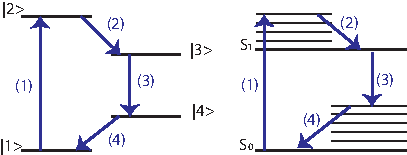
\includegraphics{./images/laserpath.pdf}

}

\caption{\label{fig-laserpath}Left: A Jablonski diagram that shows the
pathways of a four-level system. Radiative transfers of energy are the
(1) and (3) pathway; (2) and (4) are relaxation process. Right: the
intrinsic four-level system of an organic semiconductor is due to the
additional vibronic energy levels at the ground state and excited
state.}

\end{figure}

\hypertarget{laser-structures}{%
\section{Laser Structures}\label{laser-structures}}

There are a few different resonator types that enable lasing, such as
planar micro-cavities, Fabry-Perot cavities, micro-ring, microdisk, and
microspherical resonators. Though distributed feedback (DFB) resonators
can tune the wavelength by altering the period the light travels in the
optical gain material. This is done by changing the film thickness to
alter the effective refractive index. A simple OSL structure is shown in
Figure \protect\hyperlink{imagesux2flaseramp}{1.12}.

A simple organic semiconductor laser needs to have lower losses than the
total gain/amplification to achieve lasing. This total gain is dependent
on the stimulated emission cross-section \(\sigma_{em}\). The losses
depend on reabsorption or other exciton quenching pathways, as well as
cavity losses. The lasing condition is the electric field \(E_0\) of the
confined light being able to replicate the same path
\[E_0 = E_0 exp(i4\pi nL/\lambda_0)\sqrt{R_1R_2e^{2L(g-\alpha)}}\] where
\(R_1\) and \(R_2\) are the reflectivities of the mirrors \(L\) distance
apart, \(\lambda_0\) is the vacuum wavelength, \(g\) and \(\alpha\) are
the modal gain and loss respectively (Hill and Gather 2014). There must
be intervals of acceptable length L because of the imaginary component.
This condition can be written \[L = \frac{\lambda_0}{2n}m\] where m is
an integer. As mentioned previously, the modal gain \(g\) must be higher
than the combines losses, written mathematically (Hill and Gather 2014)
\[g \geq \alpha - \frac{ln(R_1R_2)}{2L}\] To understand gain better, a
look at the population dynamics of the levels. Spontaneous emission from
\(S_1\) to \(S_0\) \(N_{10}\) is governed by
\[\partial N_{10} = N_1A_{10}\partial t\] but is changed when undergoing
stimulated emission: \[\partial N_{10} = N_1u(\lambda)B_{10}\partial t\]
where \(N_1\) is the poulation of the \(S_1\) state, \(u(\lambda)\) is
the photon density, and \(A\) and \(B\) are the Einstein coefficients.
Because stimulated emission is now dependent on the Einstein coefficient
\(B\), the gain of the material is now too. And because
\(B \propto \sigma_{em}\), we have
\[\sigma_{em} = \frac{\lambda^4E_f(\lambda)}{8\pi n^2c\tau_f}\] where
\(n\) is the average refractive index of the gain medium, \(c\) is the
speed of light, \(\tau_f\) is the fluorescence lifetime of the emissive
lyaer, and \(E_f(\lambda)\) is the spectral distribution of its PLQY.
From this formula, we can see to optimise the stimulated-emission cross
section, and hence the gain, a low \(\tau_f\) (fast decay) and high PLQY
with narrow spectra is needed.

\begin{figure}

{\centering 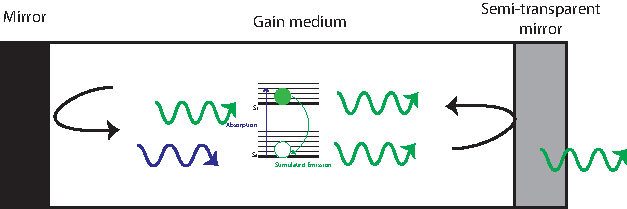
\includegraphics{./images/laseramp.pdf}

}

\caption{\label{fig-laseramp}A mirror, gain medium, semi-transparent
mirror, and an external pump source all comprise the basics of a laser.}

\end{figure}

\hypertarget{amplified-spontaneous-emission-ase}{%
\subsubsection{Amplified spontaneous emission
(ASE)}\label{amplified-spontaneous-emission-ase}}

Without needing to build a cavity, the prospect for lasing can be
evaluated by use of a simple waveguided structure that enables a weak
but intrinsic optical feedback. ASE still sees spectral narrowing of the
full-width-at-half-maximum (FWHM), but does not exhibit coherent
emission out. This is because, while population inversion has occurred,
spontaneous emission dominates the system instead of stimulation
emission.

\bookmarksetup{startatroot}

\hypertarget{literature-review}{%
\chapter{Literature Review}\label{literature-review}}

There has been a lot of commotion surrounding whether or not certain
papers have achieved coherent emission from electrically pumped organic
semiconductors. The papers claiming to have achieved lasing will be
introduced and evaluated in Section~\ref{sec-laser}. To tie this review
into the experiments in this thesis, the current triplet-triplet
annihilation (TTA) upconversion literature will be reviewed and
evaluated. Collectively, this literature review will compare alternative
materials as options to achieve lasing and argue for the present
investigation: achieving electrically pumped lasing via TTA
upconversion.

\hypertarget{sec-laser}{%
\section{Prospects of Electrically Pumping}\label{sec-laser}}

Although countless papers have published results confirming realisation
of lasing emission from electrical excitation, only a few have been
convincing, even fewer have achieved lasing, and none have achieved
stable emission. One paper claimed lasing in tetracene single crystals
(Schön et al. 2000), but was subsequently retracted as part of the Schön
scandal. Another paper (El-Nadi et al. 1998) reported a 410 nm emission
from \(Alq_3\) blended with Nile Blue, but neither of those materials
emit at the reported wavelength. It is believed to be an emission from
the indium that has an atomic line at 410 nm (I. D. W. Samuel and
Turnbull 2007). Also curiously, is the alleged lasing voltage of 0.27 V
with a threshold current of 0.088 mA in a millimeter dimension device.

\hypertarget{progress}{%
\subsection{Progress}\label{progress}}

Laser emission from a pulsed DCJTI dye doped material was reported (X.
Liu et al. 2009) sandwiched between dielectric mirrors. They report, at
a current density of \(860\ mA \ cm^{-2}\), narrowing of the emission
linewidth (2.6 nm to 2.0 nm), change in beam divergence (53 mrad to 13
mrad), and claim the threshold for optical pumping is the same for
electrical pumping. However, a paper by Samuel \emph{et al.} (Ifor D. W.
Samuel, Namdas, and Turnbull 2009) reviews the article and calls it
"puzzling". The narrowing is far too small compared to the 10-50 factor
reduction seen in microcavity OSLs. The threshold is five orders of
magnitude smaller than equivalent structures. Duarte \emph{et al.} has
strong words against this paper too (V. Duarte F. J. 2018).

Similarly, a paper by Lin \emph{et al.} (J. Lin et al. 2017) reports a
threshold of \(~2\ mA \ cm^{-2}\), which is considerably lower than any
predicted threshold from many publications. Baldo \emph{et al.} (Baldo,
Holmes, and Forrest 2002) suggests a threshold of greater than
\(5\ A \ cm^{-2}\), while Kozlov \emph{et al.} (Kozlov et al. 1997)
calculated, for a Fabry-Perot laser with a DCM-doped \(Alq_3\) emissive
layer at 5ns pulsed excitation, a threshold current density of
\(200\ A\ cm^{-2}\). \(200\ A\ cm^{-2}\) would be too high for
continuous operation but works in the pulse regime (I. D. W. Samuel and
Turnbull 2007). A distributed feedback structure works better than a
Fabry-Perot resonator, where it can reduce the threshold to an estimated
\(80\ A cm^{-2}\) (Kozlov et al. 2000).

Spatially coherent light was reported in a tandem OLED structure under a
pulse domain using Coumarin 545 T (F. J. Duarte, Liao, and Vaeth 2005).
The structure was too weak to achieve laser behaviour
(\(800 mA\ cm^{-2}\)), yet shows good prospects. Another paper, Cai
\emph{et al.} (Cai et al. 2017), reported lasing action; however
similarly to previous attempts has a low threshold (\(0.8 mA cm^{-2}\)
and line width of 0.5 nm.

A recurring theme is the failure to recognise lasing. Samuel \emph{et
al.} points out four key properties of light amplification by stimulated
emission or radiation in a resonator. The first is narrow linewidth
emission. Second is the light output comprises a beam. Third is there
will be a clear threshold (change in slope) of output power and
linewidth. Finally, the fourth is the emission will resemble the output
expected of the specific gain medium and resonator.

\hypertarget{success-at-last}{%
\subsection{Success at last}\label{success-at-last}}

In 2019 Sandanayaka \emph{et al.} (Sandanayaka et al. 2019) reported
blue lasing from an electrical excitation of a conventional OLED that
incorporated a mix-order distributed feedback \(SiO_2\) grating. OLEDs,
with high efficiency and EL emission efficiency, tend to only notably
increase EQE up to current densities of \(1\ A \ cm^{-2}\). However,
these current densities are not close to the injection of
\(1 \ kA \ cm^{-2}\) that is needed for lasing (Adachi and Sandanayaka
2020). This was their reason to use a single-layer structure containing
no heterointerface, such that excitons generated and deactivated in the
emitting layer. The mobility of the lasing material used, BSB-Cz, for
both electrons and holes was \(10^{-4}cm^2/Vs\). Sandanayaka \emph{et
al.} celebrated a constant EQE up to \(~1\ kA \ cm^{-2}\) without
drastic roll-off. As well as the polaron absorption overlap of 600 to
1000 nm, which avoids overlap of the emission spectrum of the blue (460
nm) BSB-Cz. The lasing threshold was about \(700\ A\ cm^{-2}\) with a
spectral width of 0.2 nm. The issue with this laser is that it displayed
very short device lifetime.

\hypertarget{issues}{%
\subsection{Issues}\label{issues}}

Electrically pumped lasers suffer from a whole slew of complex problems
(Tessler et al. 2000; Baldo, Holmes, and Forrest 2002; Giebink and
Forrest 2009). Forget and Chénais (Adachi and Sandanayaka 2020) ignore
the losses and assume a lower limit for calculating the current density
threshold:
\[J_{threshold} = \frac{n_s^{threshold}e}{\phi_{spin} \phi_F\tau_{rad}}\]
where \(n_{threshold}\) is the surface density of singlet excitons, e is
the elementary charge, \(\phi_{spin}\) is the exciton recombination rate
to generate singlets (fluorescence has \(\phi_{spin}=0.25\)), \(\phi_F\)
is the PLQY, and \(\tau_{rad}\) is the lifetime of radiative decay. They
assume values of \(\tau_{rad}~1ns\), and \(\phi_F~1\) to obtain the
threshold \[J_{threshold} ~ 1 kA/cm^2\] For triplet-triplet annihilation
upconversion, some materials have an upper \(\phi_{spin}\) limit of
\(0.65\). This brings the new threshold for TTU to
\[J_{TTA} ~ 0.5 kA/cm^2\] Unfortunately this is only a lower limit.
Losses will inevitably seep their way in, increasing the practical
limit. This thesis focuses on decreasing the emissive layer losses, but
a brief overview of structural losses will be included as well. The
first issue is the problematic electrical contacts that cause problems
with optical confinement. The metallic electrodes absorb the guided
mode, an absorption that is enhanced by the similar refractive indices
of organic molecules. This loss further reduces the light out. Some
methods have been used to reduce the overlap between the optical mode
and the electrode (Reufer et al. 2004; Lattante et al. 2006; B. H.
Wallikewitz et al. 2010; Görrn et al. 2007). There are bountiful
polarons present at high current densities. Unfortunately they have a
broad absorption band, meaning they overlap with the emission spectra
and can quench the emission (Baldo, Holmes, and Forrest 2002). Both
electrical contact issues and polaron absorption can be resolved with
higher mobility. Organic light-emitting field-effect transistors
(OLEFETs) show potential to fix these problems simultaneously (Muccini
2006), but OLEFETs are outside the scope of this thesis.

The loss that this thesis focus on is the triplet exciton issue -- by
far the most difficult to overcome. Not only does electrical pumping
directly generate triplets, but triplets have much longer lifetimes
(\textasciitilde{}\(ms\) (Marcus Lehnhardt et al. 2011)), causing
pile-up in long-pulse or high repetition-rate regime (Forget and Chénais
2013). Even under the more favourable short pulse regime (S. Schols et
al. 2010), triplets still cause issues such as absorbing laser photons
(triplet absorption), or quench singlets (singlet-triplet annihilation)
(Giebink and Forrest 2009). Giebink \emph{et al.} (Giebink and Forrest
2009) showed that STA was the dominant mechanism, and TA. Lehnhaardt
\emph{et al.} (M. Lehnhardt et al. 2010) showed STA and TA induce losses
in guest/host systems.

\hypertarget{design-rules-for-organic-laser-diodes}{%
\subsection{Design rules for organic laser
diodes}\label{design-rules-for-organic-laser-diodes}}

To summarise the losses, this section aims to elaborate on the design
rules that must be kept in mind when trying to realise OSLs.

\hypertarget{balanced-carrier-mobilities}{%
\subsubsection{Balanced carrier
mobilities}\label{balanced-carrier-mobilities}}

At high excitation, high charge carrier mobility is vital to reduce the
losses, such as bimolecular annihilations, induced absorption losses,and
field-induced exciton dissociation (Gärtner 2009). One simulation
predicted carrier mobilities of at least \(5\times10^{-2}cm^2/Vs\) to
achieve a lasing input of \(10kA/cm^2\) (Gärtner 2009). Furthermore, the
mobilities of both electrons and holes need to be balanced. If not,
exciton recombination will not happen in the emissive layer because the
lower mobility charge will only be injected a few nanometers into the
emissive layer (Gärtner 2009). Hence, thicker emissive layers will
reduce bimolecular annihilation processes.

\hypertarget{guest-host}{%
\subsubsection{Guest-Host}\label{guest-host}}

Gust-host systems enable low self-absorption because of the separate
emission/absorption energies. Host-guest systems will also reduce
field-induced exciton dissociation, while maintaining a high singlet
exciton density (Gärtner 2009).

\hypertarget{pulse-operation}{%
\subsubsection{Pulse operation}\label{pulse-operation}}

Joule heating degrades the emissive layer, a process that DC operation
amplifies. Pulse measurements not only will reduce this heating, but it
also enables triplets to decay before triplet absorption dominates.

\hypertarget{triplet-dynamics}{%
\subsection{Triplet Dynamics}\label{triplet-dynamics}}

If we are to ever realise electrically pumped lasers, triplets and their
usually not luminescent property, must be managed. Harvesting emission
from triplets via phosphorescence (Baldo et al. 1998) was a promising
turning point for OLEDs because it increased the internal quantum
efficiency (IQE) from \(25\%\) to an achievable \(100\%\). Triplet
dynamics have been understood to be a great obstacle in organic lasing
(Reufer, Lupton, and Scherf 2006; M. Lehnhardt et al. 2010; Zhang and
Forrest 2011), especially electrically pumped (Baldo, Holmes, and
Forrest 2002; Zhang, Lee, and Forrest 2014; Giebink, Sun, and Forrest
2006). Some ways around managing triplets are by adding " triplet
scavengers" (S. Schols et al. 2009) or "triplet managers" (Zhang and
Forrest 2011), or a way that managed to remove triplets with "plasmonic
sinks" (Kéna-Cohen et al. 2011).

The triplet state \(T_1\) is the lowest energy of some \(T_n\) number of
triplet states. Triplets \(T_1\) usually decay to the ground state but
can undergo a photon absorption and be excited to a higher energy
triplet state via a process called triplet absorption (TA). \(80\%\) of
the time this excited state relaxes back to the \(T_1\) rapidly (300 fs
timescale), but the remaining percent dissociate into charges (Yang et
al. 2009). We can start seeing that the the long-lived triplet
population from instant generation of triplets and ISC triplets dominate
the exciton population in electrically injected systems. Hence, managing
these usually non-emissive triplets is essential. This is where we
utilise the fact that a chromophore in a solid-state material always has
neighbours. TTU-based OLEDs show IQEs of up to \(62.5\%\) (Zhang and
Forrest 2012; Di et al. 2017), which is not the \(100\%\) phosphorescent
or TADF molecules.

\hypertarget{sub:phos}{%
\subsubsection{Why not phosphorescence?}\label{sub:phos}}

Phosphorescence on a casual glance might seem very enticing for
electrically pumped lasers due to the triplet problem. You might ask
yourself: If phosphorescence is able to emit light via the triplet state
\(T_1\) and the singlet state \(S_0\), then under electrical excitation
we can utilise the favoured triplets to obtain an \(100\%\) internal
quantum efficiency (IQE)? Well we can first consider each colour. Red
emitters would have to compete with nonradiative decay because of the
energy-gap law. Blue emitters suffer from being unstable due to the
higher energy of the singlet state lying in the UV range. To now cut
green from the equation, the additional losses must be considered.

For a laser, triplet absorption must be avoided. From the Köhler and
Bässler rule of thumb (Stuke 1992), the stimulated emission
\(T_1 \rightarrow S_1\) directly competes with \(T_1 \rightarrow T_n\)
absorption. Typically, the overlap of these spectral bands is very high
for these two process, which causes phosphorescence to struggle in
achieving electrically pumped lasing (Forget and Chénais 2013). A
material would need to not only exhibit strong spin-orbit coupling to
enable phosphorescence, but also to have the emission spectrum shifted
from the triplet absorption spectrum (Forget and Chénais 2013). Jenekhe
\emph{et al.} (Jenekhe 1986) attempted a Ir(ppy)3 phosphorescent emitter
and Schols (Sarah Schols 2011) attempted a Btp2Ir(acac) phosphorescent
emitter to observe Amplified Spontaneous Emission (ASE). Both were met
with nothing promising.

\hypertarget{is-triplet-triplet-upconversion-the-way-forward}{%
\subsection{Is triplet-triplet upconversion the way
forward?}\label{is-triplet-triplet-upconversion-the-way-forward}}

TTA molecules display efficient blue emission, minimal EQE roll off,
lower operation voltage, and low processing cost (Denis Y. Kondakov
2009; Popovic and Aziz 2005; Luo, Lu, and Huang 2016; Qiao and Ma 2020;
Zhu and Yang 2013; Denis Y. Kondakov 2015). Typical OLEDs express a EQE
roll off due to losses such as STA, SPA, and loss of charge carrier
balance (Soman, M, and Unni 2018), yet in a TTU-based OLED, TTA
upconversion counteracts these processes. Molecules that exhibit
efficient TTA upconversion must have these requirements

\begin{enumerate}
\def\labelenumi{\arabic{enumi}.}
\item
  Singlet energy level lower than two triplet states
  (\(S_n \leq 2 \times T_1\))
\item
  Long triplet lifetime
\item
  TTA that cannot access the second triplet excited-state \(T_2\)
\end{enumerate}

The molecules that meet these requirements come under the polycyclic
aromatic hydrocarbon acenes, such as antrhracene, tetracene, rubrene,
and their derivatives (Gao et al. 2021, 2019; Jing Zhou et al. 2015;
Dzebo et al. 2016; Keivanidis et al. 2009; Serevičius et al. 2014). An
efficient aluminium complex (\(Almq_3\)) doped with coumarin6 OLED had
an EQE of \(7.1\%\) (Kido and Iizumi 1998) -- the first device to
surpass the fluorescent limit by using TTU.

\hypertarget{ttu-as-host}{%
\subsubsection{TTU as host}\label{ttu-as-host}}

Molecules that exhibit TTU generally suffer from low PLQY because of
aggregation induced quenching or excimer formation (Gao et al. 2021).
Thus these materials can be used in OLEDs as a host to produce efficient
devices that emit at the guest's wavelength (Köhler and Bässler 2009;
Kuma and Hosokawa 2014; Chou et al. 2014; Lim et al. 2019). The excitons
are formed directly on the host and then the singlets (both direct and
TTU singlets) are transferred via FRET to the guest for emission. It is
necessary that the overlap of anthracene units between neighbouring
molecules are reduced (Fukagawa et al. 2012).

\hypertarget{ttu-as-guest}{%
\subsubsection{TTU as guest}\label{ttu-as-guest}}

Not only can TTU be used a host, but it can be used as a guest to
improve the EQE of a non-doped device. Many devices with high EQEs
(\textgreater10\%) have been fabricated with TTU as a guest (Chou et al.
2014; Y.-H. Chen et al. 2016; Kabra et al. 2010; Y. H. Kim et al. 2001).
There have also been devices with TTU as both the host and guest (Jie
Zhou et al. 2014; Zheng et al. 2015).

\hypertarget{neat-film-ttu}{%
\subsubsection{Neat film TTU}\label{neat-film-ttu}}

In an attempt to simplify the device structure and fabrication process,
while avoiding parasitic energy loss (Gao et al. 2021), non-doped TTU
devices have also been fabricated (X. Tang et al. 2018; H. Liu et al.
2019). They have seen high EQEs, some of the highest in non-doped
devices (\(10\%\)) (W. Liu et al. 2019).

\hypertarget{ttu-in-lasers}{%
\subsubsection{TTU in Lasers}\label{ttu-in-lasers}}

Triplet-Triplet annihilation upconversion has not seen extensive
development when it comes to organic lasers (Atul et al. 2021). The
ultrafast lifetime of upconversion provides more excitement for the
realisation of lasers than TADF molecules that display slow RISC
lifetimes. So it is likely the limited \(62.5_max\) IQE present in TTU
devices that has shunned away researchers. This thesis aims to
demonstrate the promise of using TTU as a mechanism to manage the
triplet excitons for the purpose of electrically pumped lasers.

\hypertarget{ttu-in-this-thesis}{%
\subsubsection{TTU in this thesis}\label{ttu-in-this-thesis}}

This thesis considers first neat film molecule with the aim in showing
that it has triplet-triplet annihilation upconversion. To analyse the
requirement that TTU needs close range DET transfers to efficiently
perform, the TTU material is doped in a large weight percentage as a
guest in a host. This separates the TTU chromophores, resulting in
limited DET transfer and subsequently lowering the TTU rate. Hence it
will show the molecule's dependence on nearby neighbouring chromophores.
Then the TTU molecule will be doped as the host into a lasing material
to improve the PLQY of the device and show TTU enhanced devices can be
possible. Even though doping affects the charge mobilities of the system
(S.-B. Lee et al. 2003), the increased PLQY should see positive results.

\bookmarksetup{startatroot}

\hypertarget{experimental-method-and-materials}{%
\chapter[ Experimental Method and
Materials]{\texorpdfstring{\protect\hypertarget{sec:exp}{}{}
Experimental Method and
Materials}{ Experimental Method and Materials}}\label{experimental-method-and-materials}}

This chapter will describe the methodology of device fabrication and the
materials used. Fabrication of organic light emitting diodes were the
principle experiment. So this chapter will include the steps of
fabrication, along with the analysis and testing of said devices. The
number of devices tests, and number of measurements, along with
uncertainty will be spoken about in their respective chapters.

\hypertarget{materials}{%
\section{Materials}\label{materials}}

The organic semiconductor materials that were used in this thesis were
primarily small molecular organic semiconductors. All of these layers
were thermally evaporated under vacuum.

\hypertarget{oled-fabrication}{%
\section{OLED Fabrication}\label{oled-fabrication}}

All fabrication was conducted within the Class 1000 clean room at the
Centre of Organic Photonics and Electronics (COPE) at The University of
Queensland. The Queensland Node of the Australian National Fabrication
Faacility (ANFF) maintained and established some of the procedures and
equipment that was also needed to complete fabrication. All OLEDs in
this thesis were fabricated using thermal evaporation

\hypertarget{cleaning-substrates}{%
\subsection{Cleaning substrates}\label{cleaning-substrates}}

To begin, OLEDs need to have transparent window to view the light from.
A pre-patterned indium tin oxide (ITO) layer on a 100 nm thick glass
substrate was used as the window. They were sourced from Xin Yan
Technology and require cleaning before deposition of organic layers to
improve charge injection into the emissive layer. The cleaning process
follows these sequential steps.

\begin{enumerate}
\def\labelenumi{\arabic{enumi}.}
\item
  Sonicate substrates in dionised (DI) water with detergent (Alconox)
  for 5 minutees
\item
  Heat substrates at 150 \(\degree C\) for 15 minutes in same DI water
  with Alconox
\item
  Sonicate substrates in DI water for 5 minutes
\item
  Sonicate substrates in Acetone for 5 minutes
\item
  Sonicate substrates in Isoproponaol for 5 minutes
\item
  Blow dried with high pressure nitrogen gun
\item
  UV-Ozone treatment for 45 minutes
\end{enumerate}

The culmination of the cleaning with UV-Ozone is to remove the organic
impurities and improve the wetibility of the substrates.

\hypertarget{layer-deposition}{%
\subsection{Layer Deposition}\label{layer-deposition}}

The hole transport layer is the first layer to be deposited onto the
clean substrate. Followed by the emissive layer. In the case of
host/guest systems, the emissive layer involved simultaneous thermal
deposition. The electron transport layer is deposited next. Finally
capped off with the cathode deposition. To obtain the desired area of
emission, a laser cut steel stencil was placed over the devices. There
are a few sizes of the active areas (pixels), but in this report
\(0.3 mm^2\), \(0.75 mm^2\), and \(4 mm^2\) were used.

\hypertarget{thermal-evaporation}{%
\subsection{Thermal Evaporation}\label{thermal-evaporation}}

The thermal evaporation equipment (MBraun Inert-gas Systeme, Gmbh) could
reach a vacuum of \(~10^{-6} mbar\), which enabled for organic materials
to be heated (evaporated) onto the pre-cleaned substrates. To heat the
organic materials a voltage was passed to the aluminium oxide crucibles
(1 \& 2) that contained the powered form of the material (see
Figure~\ref{fig-evap}). Inorganic materials (Calcium and Aluminium) were
deposited in different holders (5 \& 6). Two Quartz Crystal Monitors
(QCM, 8 \& 9) measured the rate of deposition, which enabled calculation
of deposition thickness. In order to deposit the layers uniformly, not
only were the substrates put in a rotatable holder (11) that could close
off deposition (10) if need be, but a specified calibration factor for
each material was used to predict consistent deposition. The evaporation
rates were kept between \(0.1-1\) Å/s to avoid piercing the layer
beneath. Additional covers (3, 4 \& 7) were used as safety in case of
sudden increase of deposition rate. Previous experiments have provided
accuracy of the QCM-measured thickness by using a Dektak XT profilometer
(Bruker) to scratch the film and measure the step distance between the
top surface of the film and substrate.

\begin{figure}

{\centering 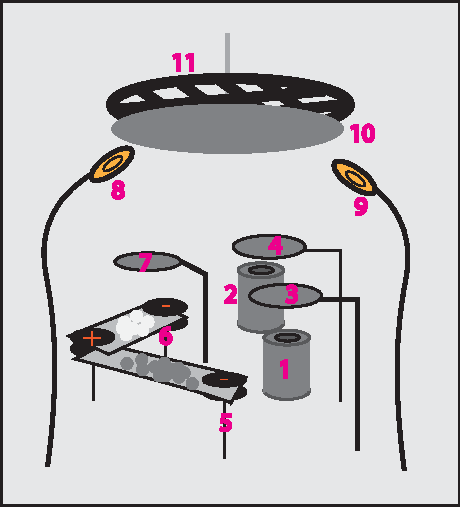
\includegraphics{./images/ThermalEvap.pdf}

}

\caption{\label{fig-evap}Schematic representation of the vacuum thermal
evaporation chamber used to deposit thin films. Aluminium and calcium
sit upon metal holders that have a current passed through it to heat it
up (5 \& 6). See text for more details.}

\end{figure}

\hypertarget{dc-measurements-1}{%
\subsection{DC Measurements}\label{dc-measurements-1}}

Two separate apparatuses were used to measure DC measurements of the
OLEDs, depending on the size of heir emission area. For \(4mm^2\) areas,
the devices were placed within an integrating sphere (Hamamatsu
Photonics C9920-12) coupled with a Keithley 2400 source meter. The
Electroluminescence spectra was recorded using a fibre coupled PMA-12
Photonic multi-channel analyser. These measurements were performed in a
nitrogen-filled glove-box with low \(O_2\) and moisture content.

The small area devices (\(0.75mm^2\) and \(0.3mm^2\)) needed to be
encapsulated so that they could be transported to the transient response
apparatus. These OLEDs were tested with a pre-calibrated photomultiplier
tube (PMT, Hamamatsu H10721-20) coupled with a Keithley 2400 source
meter. The electroluminescence spectra was measured with a CCD
spectrometer (Thor labs, CCS100). A LabVIEW program could collate the
voltage, current, luminance, and spectra to calculate the external
quantum efficiency (EQE).

The PMT first needed to be calibrated to convert photocurrent into
luminance. This was done by setting the distance between the PMT and
device to a fixed value for a given emissive pixel area A. To verify the
calibration it is possible to use a luminance meter (Konica Minolta
LS100). The calibration factor scales the relationship between
photocurrent and pixel area A to give luminance L.

Total luminance L output is not the same brightness that the human eye
sees because of how the eye responds to different wavelengths. The total
power of the emitted signal the human recognises is given by
\[Power = \frac{\phi_{lum}}{683}\times \frac{\int EL(\lambda)d\lambda}{\int ER(\lambda)\times EL(\lambda)d\lambda}\]
where \(\phi_{lum} = \pi\times L \times A\), \(EL(\lambda)\) is the
normalised distribution of the electroluminescence signal,
\(ER(\lambda)\) is the eye response function, and the \(683 lm/W\)
constant is the flux at the peak wavelength of 555nm of \(ER(\lambda)\).
This power can then be used to calculate the number of photons (\(n_p\))
emitted by the device using
\[n_p = \frac{\int EL(\lambda)\lambda d\lambda}{\int ER(\lambda)\times EL(\lambda)d\lambda} \times \frac{1}{hc} \times Power\]
where \(h\) and \(c\) are Planck's constant and the speed of light
respectively. Comparing this to the current \(I=e\times n_e\), a ratio
of number of electrons \(n_e\) injected to total number of photons out
\(n_e\) provides us with the definition of external quantum efficiency
(EQE). Refer to Figure~\ref{fig-perfo} to see the J-V-L characteristics
of a test OLED with Super Yellow as the emissive layer.

\begin{figure}

{\centering 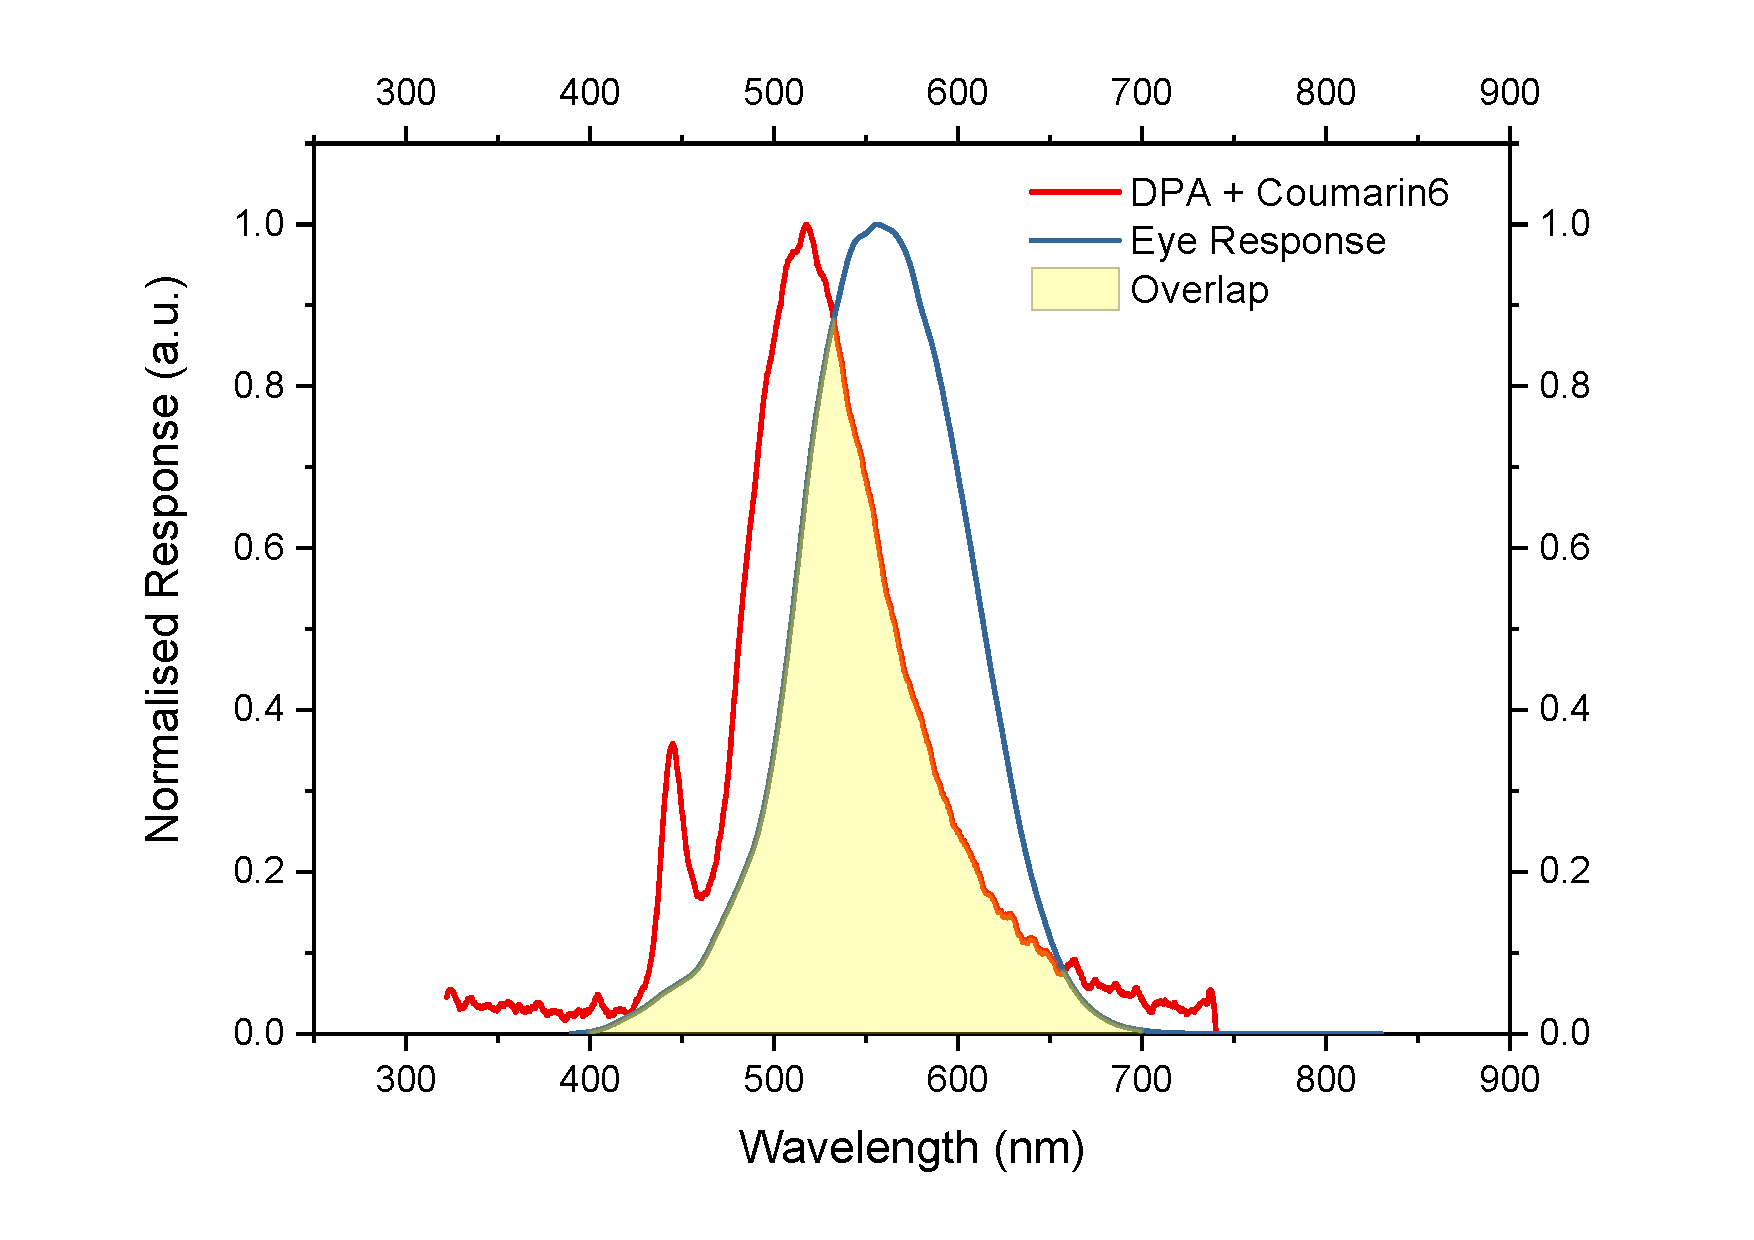
\includegraphics{./images/EyeResponse.pdf}

}

\caption{\label{fig-eye}Normalised eye response curve as per the CIE
1931 standard in relation to the emission spectra of DPA/Coumarin6
host/guest system that can be found in the final section.}

\end{figure}

\hypertarget{pulse-measurements-1}{%
\subsection{Pulse Measurements}\label{pulse-measurements-1}}

\begin{figure}

{\centering 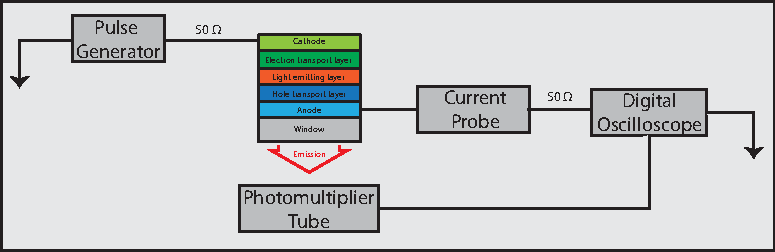
\includegraphics{./images/Pulse.pdf}

}

\caption{\label{fig-pulse}Schematic diagram of high voltage pulse
measurement apparatus. Reduction of signal reflection was achieved by
using 50 {Ω} resistance cables and terminating the instruments at the
same resistance.}

\end{figure}

Lasing required pulse measurements due to the need to inject high
current densities without massive losses, such as Joule heating and
avoid long triplet exciton times. So testing the OLED devices under a
pulse regime is necessary to elucidate the transient behaviour. Pulse
widths range from nanosecond to microsecond lifetime to observe the
non-linear processes such as charge transport, exciton formation, and
exciton annihilation processes (TTA).

To output voltage pulses, high-speed electrical pulse generators
(AV-1011B1-B) and AVTECH AVRK-3-B) were utilised to deliver pulses with
maximum 500 V, 3-6 ns rise and fall times, and 1 kHz operational
frequency (see Figure~\ref{fig-pulse}). The current was measured using a
ultra fast current probe (Integrated Sensor Technology, 711 UHF) that
fed, as well as the electroluminescence response (PMT), into a digital
oscilloscope (Teledyne LeCroy) with resolution of 2 GHz. The cables
connecting each equipment piece had resistance of \(50 \Omega\) and
placed without bends to reduce wave-guided losses and current
reflections.

\bookmarksetup{startatroot}

\hypertarget{confirmation-of-triplet-triplet-upconversion-in-26-dpa}{%
\chapter[ Confirmation of Triplet-Triplet Upconversion in
2,6-DPA]{\texorpdfstring{\protect\hypertarget{sec:level3}{}{}
Confirmation of Triplet-Triplet Upconversion in
2,6-DPA}{ Confirmation of Triplet-Triplet Upconversion in 2,6-DPA}}\label{confirmation-of-triplet-triplet-upconversion-in-26-dpa}}

\hypertarget{introduction}{%
\section{Introduction}\label{introduction}}

In this section, I investigated the electroluminescence properties of a
model anthracene derivative 2,6-diphenylanthracene (2,6-DPA) (J. Liu,
Zhang, et al. 2015; J. Liu, Dong, et al. 2015) (see
Figure~\ref{fig-dpa}\}), as well as 10wt\% 2,6-DPA doped as a host in
3,3'-Di(9H-carbazol-9-yl)-1,1'-biphenyl (mCBP, isomer of CBP) (see
Figure~\ref{fig-mcbp}) (Ying et al. 2018; Y. Chen et al. 2017; Ihn et
al. 2017). The OLED structure can be found in Appendix
\protect\hyperlink{apen:oledex}{{[}apen:oledex{]}}. 2,6-DPA was based in
OLEDs in neat and doped emissive layers, which their performance was
analysed under steady state and nanosecond pulse excitation. The high
\(wt\%\) of mCBP host doped into the layer is used to separate the
chromophores of 2,6-DPA. Herein, I found that 2,6-DPA exhibits the TTU
mechanism to generate extra singlet excitons, while the host-guest
system fails to exhibit TTU, as expected. At low-current densities (J)
the EQE of the device increases proportionally to \(J\) because of the
absence of dominating singlet-triplet annihilation (STA). At high
current densities, STA becomes a significant loss causing a reduction in
EQE and gain.

\begin{figure}

\begin{minipage}[b]{0.40\linewidth}

{\centering 

\raisebox{-\height}{

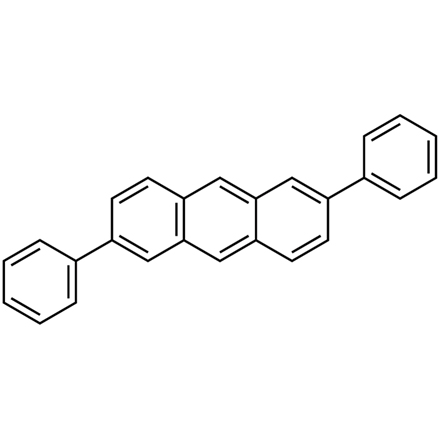
\includegraphics{./images/DPA.jpg}

}

\caption{\label{fig-dpa}Chemical structure of 2,6-DPA}

}

\end{minipage}%
%
\begin{minipage}[b]{0.60\linewidth}

{\centering 

\raisebox{-\height}{

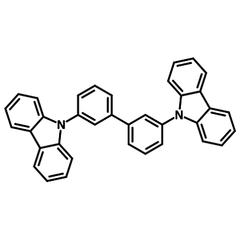
\includegraphics{./images/mCBP.png}

}

\caption{\label{fig-mcbp}chemical structure of mCBP}

}

\end{minipage}%
\newline
\begin{minipage}[b]{\linewidth}

{\centering 

\raisebox{-\height}{

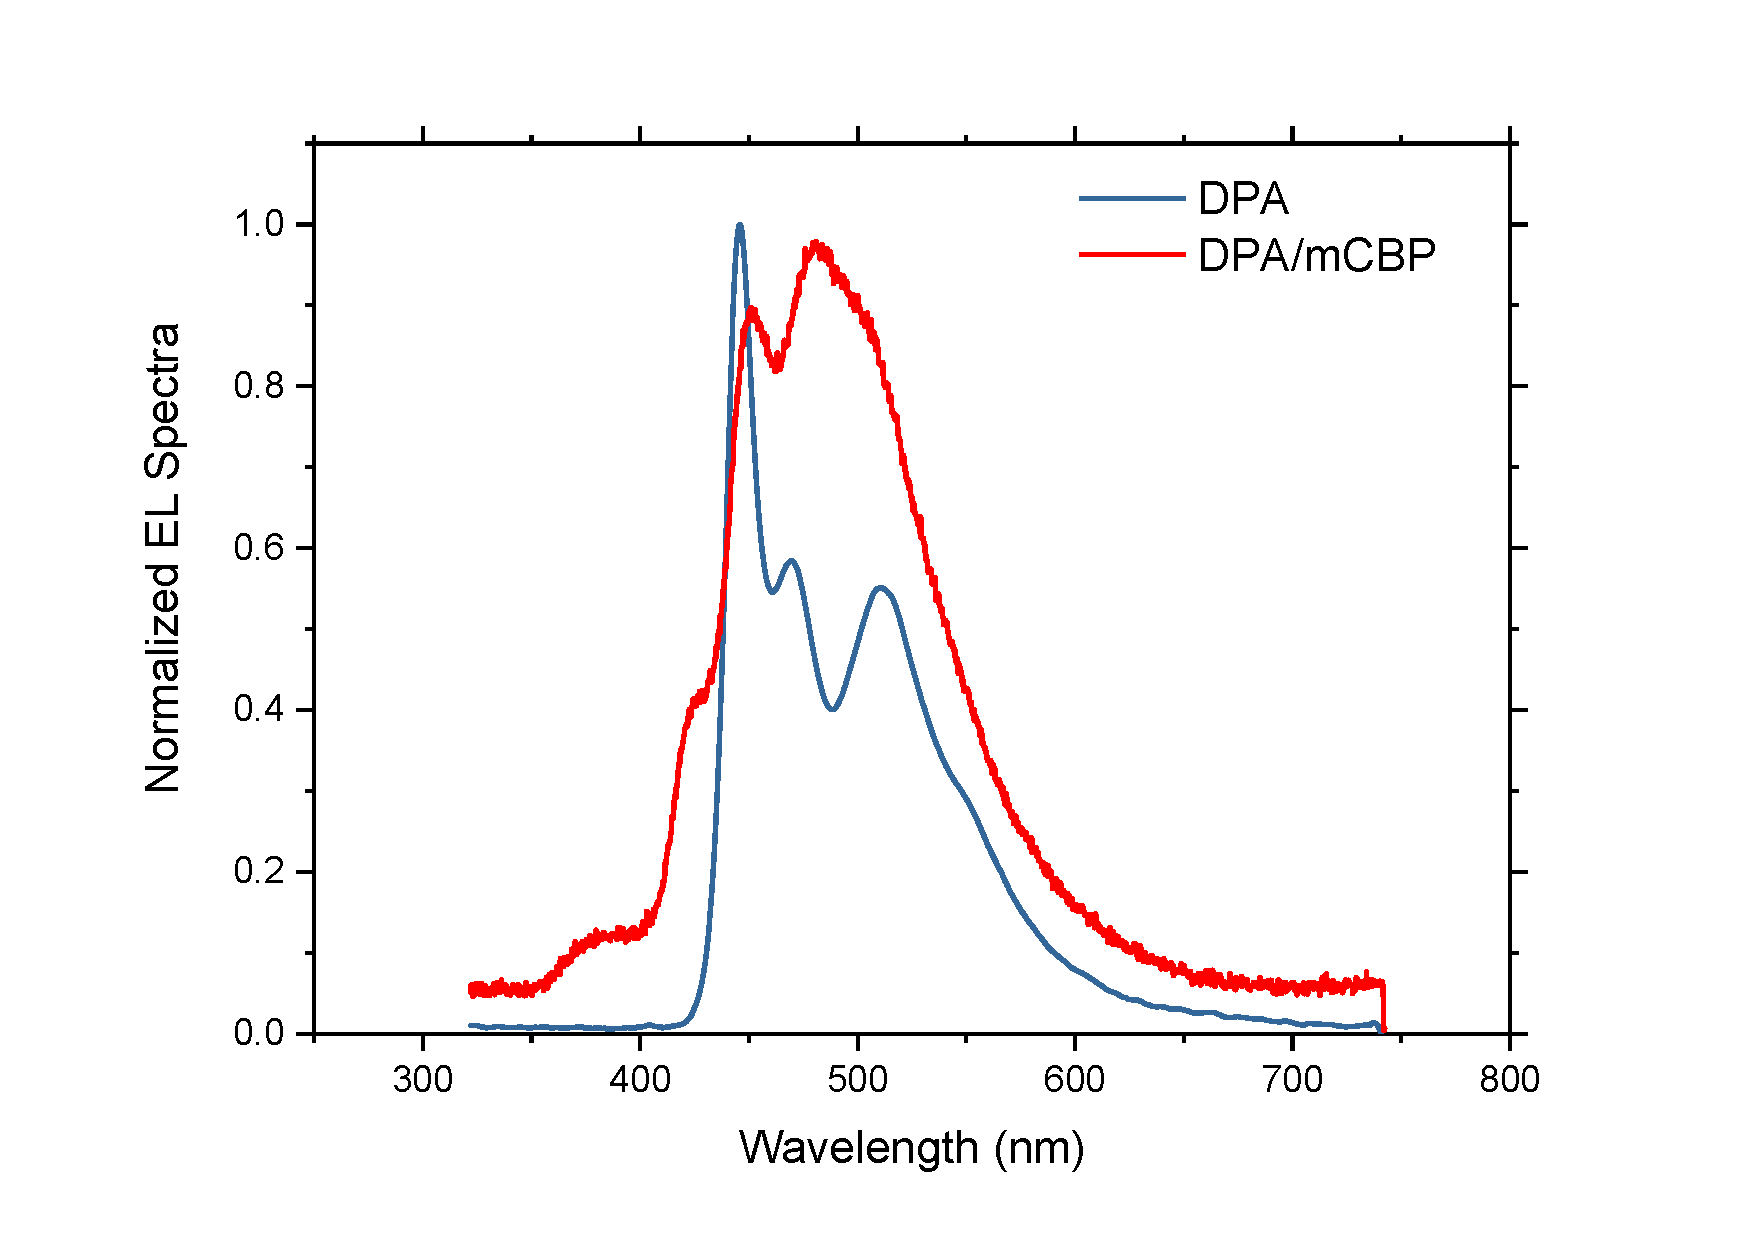
\includegraphics{./images/DPAMCBPSPEC.pdf}

}

\caption{\label{fig-dpasepc}Normalised electroluminescence (EL) spectra
for 2,6-DPA neat film and host-guest 2,6-DPA/mCBP (10wt\%)}

}

\end{minipage}%
\newline
\begin{minipage}[b]{\linewidth}

{\centering 

\raisebox{-\height}{

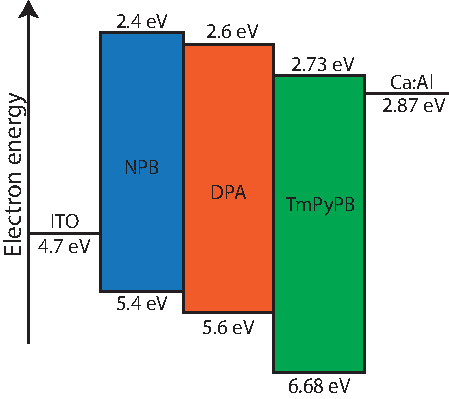
\includegraphics{./images/dpaenergy.pdf}

}

\caption{\label{fig-dpaenergy}The energy-level diagram of OLEDs based on
2,6-DPA}

}

\end{minipage}%
\newline
\begin{minipage}[b]{\linewidth}

{\centering 

\raisebox{-\height}{

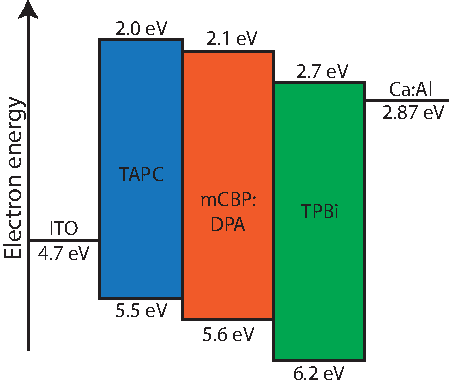
\includegraphics{./images/mcbpenergy.pdf}

}

\caption{\label{fig-mcbpenergy}The energy-level diagram of OLEDs based
on 2,6-DPA/mCBP}

}

\end{minipage}%

\end{figure}

\hypertarget{results}{%
\section{Results}\label{results}}

The OLED devices that were creates followed the structure, Indium Tin
Oxide (ITO) 100nm /
N,N'-Di(1-naphthyl)-N,N'-diphenyl-(1,1'-biphenyl)-4,4'-diamine (NPB)
40nm / 2,6-DPA 40nm / 1,3,5-Tris(3-pyridyl-3-phenyl)benzene (TmPyPB)
30nm / Calcium 5nm / Aluminum 100nm (see Figure~\ref{fig-dpaenergy}).
Each layer was thermally evaporated under high vacuum (\(10^-6 mbar)\)
without break to avoid atmosphere exposure. To achieve \(10wt\%\) , a
simultaneous doping of mCBP and 2,6-DPA with deposition rates \(0.1Å/s\)
and \(1Å/s\) was required. The deposition rate for the organic layers
were between \(0.3 - 0.6Å/s\). Within the device (see
Figure~\ref{fig-dpaenergy}), there is a substantial hole injection
barrier, enabling an accumulation of holes at the DPA/TmPyPB interface.
The thickness and structure was chosen as per the OLEDs made in Ref.
(\textbf{39?}), where they found 40nm DPA layers performed best. The NPB
layer has excellent energy level alignment to facilitate hole-injection
and transport (Shi and Tang 2002). Calcium is similar to Lithium
Fluoride (LiF) in terms of energy level, so it was used instead a the
buffer layer. Hole-blocking and electron transport layer were decided as
TmPyPB because of the deep HOMO and matching LUMO energy levels. Such a
step-wise energy level diagram enables efficient injection and transport
of charge carriers. The spectra showed a strong blue emission (peak 445
nm), matching the characteristic anthracene blue. The amorphous 2,6-DPA
has a smaller peak at 510 nm.

\begin{figure}

\begin{minipage}[t]{0.50\linewidth}

{\centering 

\raisebox{-\height}{

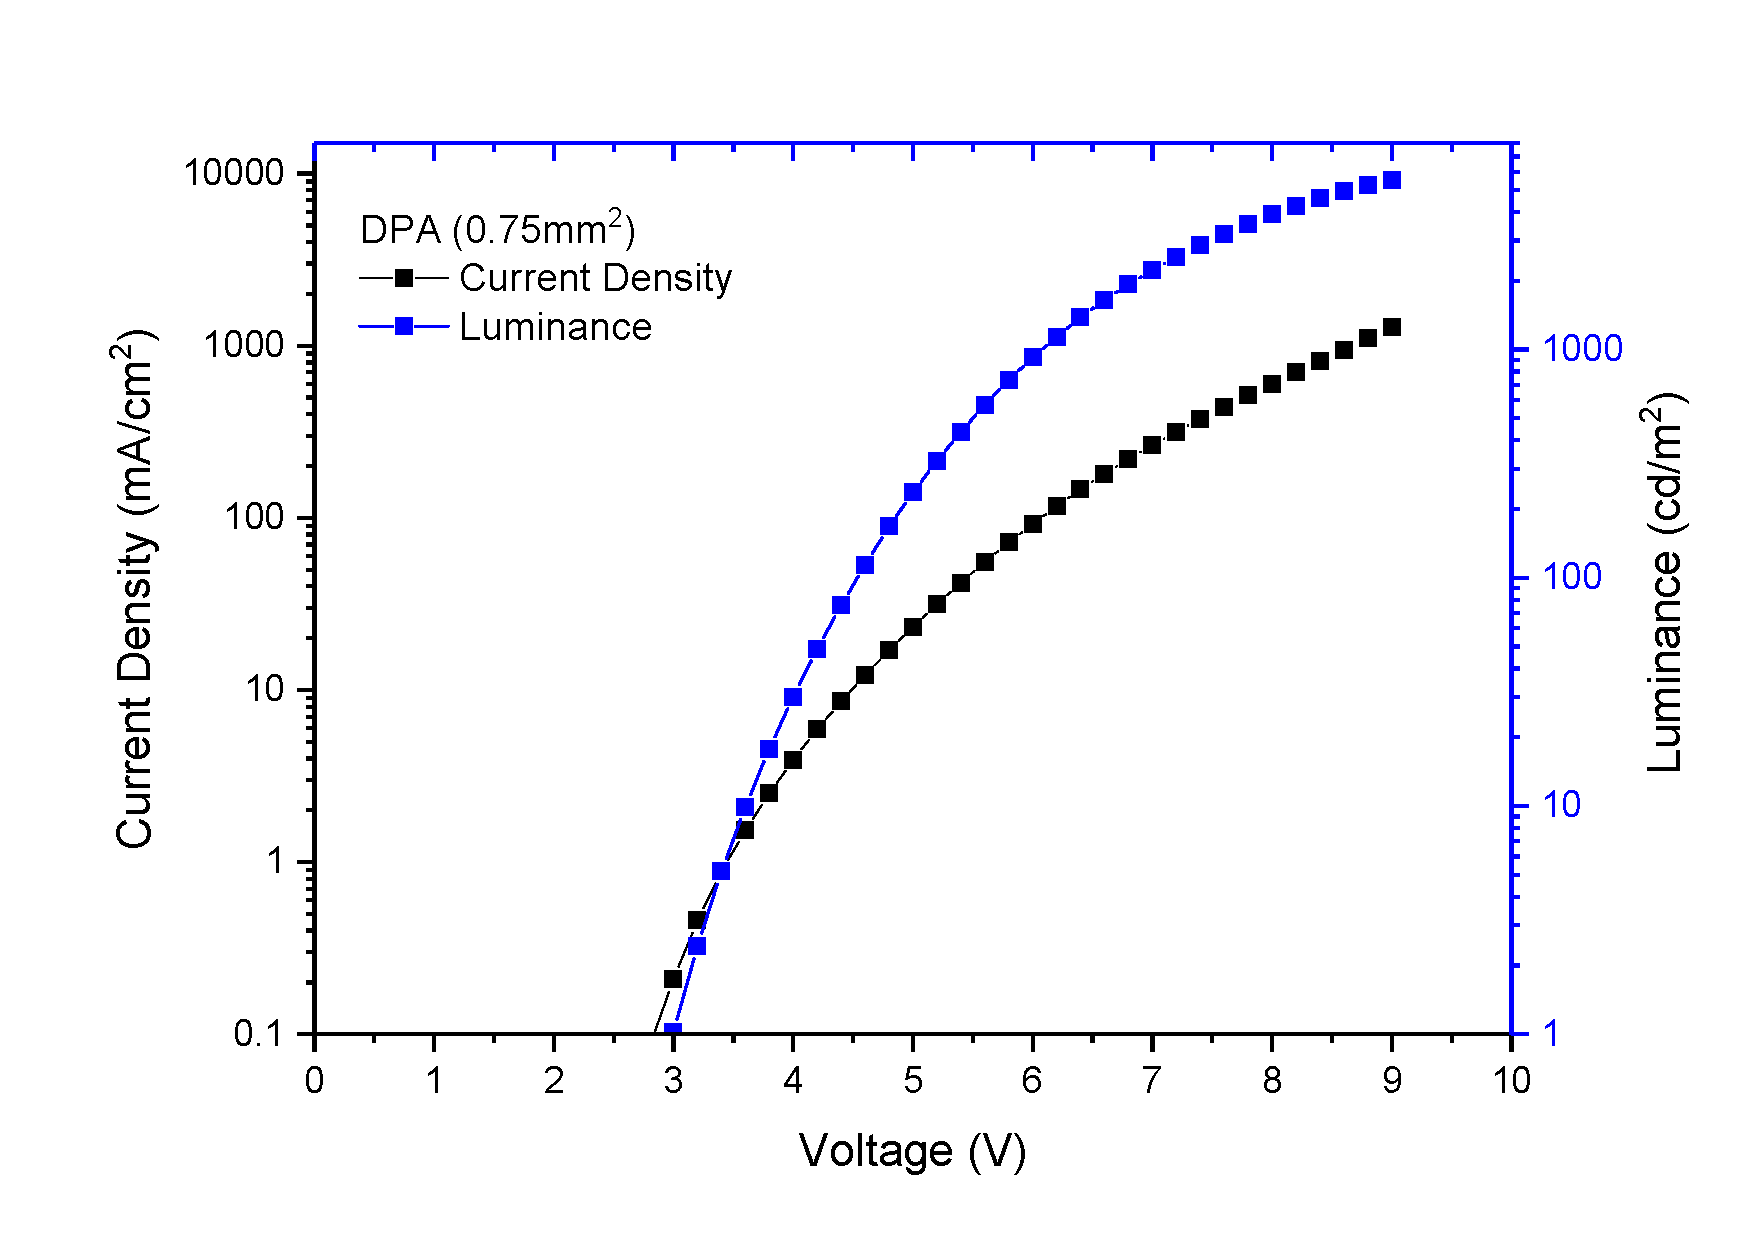
\includegraphics{./images/DPAJVL.pdf}

}

\caption{\label{fig-dpajvl}Current density-luminance-voltage (J-V-L)
graph of 2,6-DPA neat films}

}

\end{minipage}%
%
\begin{minipage}[t]{0.50\linewidth}

{\centering 

\raisebox{-\height}{

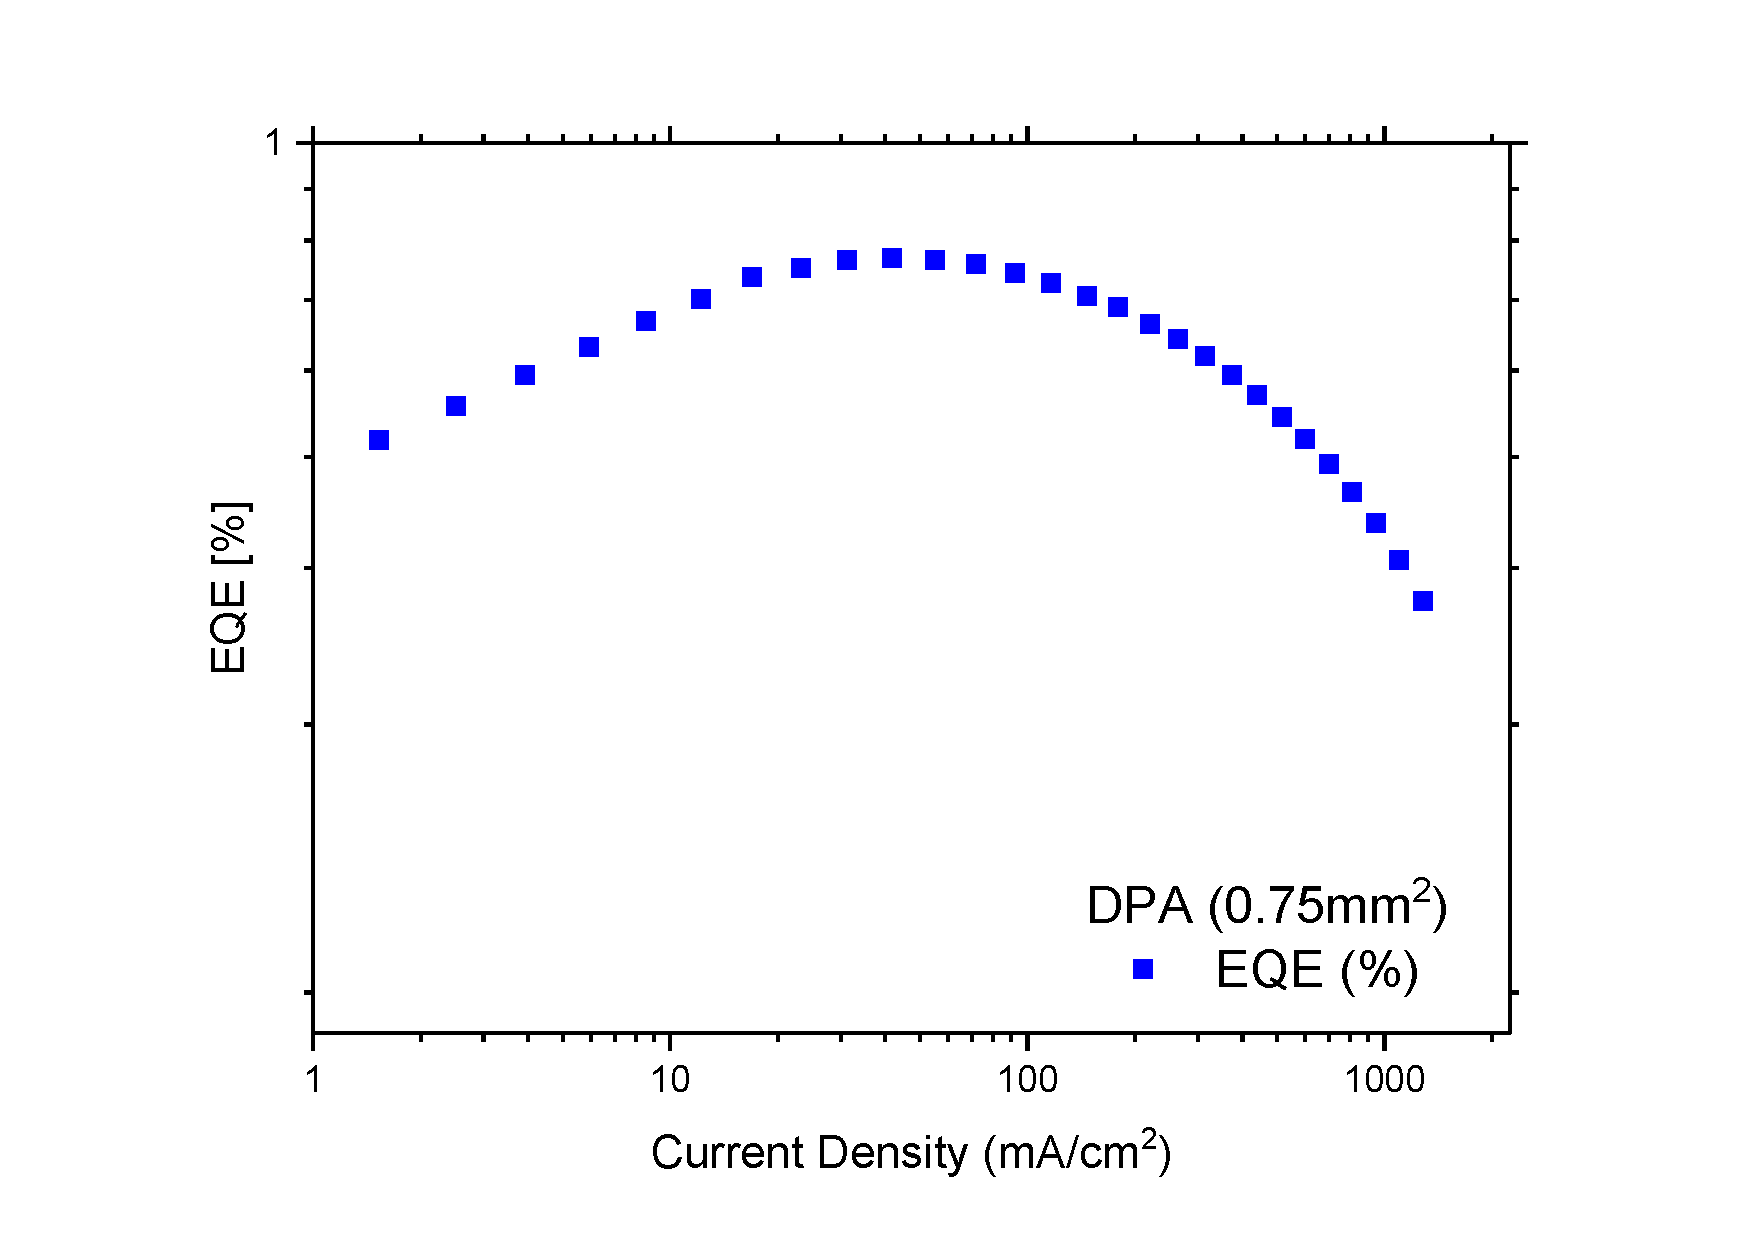
\includegraphics{./images/DPAEQE.pdf}

}

\caption{\label{fig-dpaege}EQE versus current density graph of 2,6-DPA
neat films}

}

\end{minipage}%

\end{figure}

Measurements of voltage were in increments of 0.2 V and up to 10 V in DC
measurements to observe refined characteristic curves before Joule
heating degrades the device. Four neat film devices were fabricated each
having eight pixels (four \(0.75mm^2\) and four \(0.3mm^2\)). Due to
faulty contacts, thermal evaporation alignment issues, and scratches or
blemishes on the substrate window some pixels become unable to be
tested. Others can degrade whilst a voltage is applied. The J-V-L graph
of four different pixels, as well as their EQE graph, can be found in
Appendix \protect\hyperlink{apen:dpaextr}{{[}apen:dpaextr{]}}. A turn-on
voltage of \(3.1\pm0.1\) V was achieved at the defined \(1 cd/m^2\),
with the maximum brightness approaching \(4500\pm500 cd/m^2\) at
\(9\pm0.2\) V. The J-V-L characteristics of neat-film 2,6-DPA and the
EQE versus current density graph can be found in
Figure~\ref{fig-dpajvl}. A roll up of EQE (peak \(0.7\pm0.1\)\%) until
\(~40\pm10 mA/cm^2\) demonstrates early triplet-triplet upconversion
gain (see Figure~\ref{fig-dpaege}). The peak EQE of these 2,6-DPA
devices, however, do not exceed the theoretical maximum EQE of \(2.1\%\)
(calculated using the PLQY of \(41.2\%\) (J. Liu, Zhang, et al. 2015)).

The doped 2,6-DPA in 10wt\% of mCBP devices were thermally evaporated,
following the structure: Indium Tin Oxide (ITO) 100nm /
1,1-Bis{[}(di-4-tolylamino)phenyl{]}cyclohexane (TAPC) 35nm /
2,6-DPA/mCBP (10wt\%) 40nm /
2,2',2''-(1,3,5-Benzinetriyl)-tris(1-phenyl-1-H-benzimidazole) (TPBi)
65nm / Calcium 5nm / Aluminum 100nm (see Figure~\ref{fig-mcbpenergy}).
These doped devices were meant as a comparison for non-exhibiting TTU
devices. Their J-V-L characteristics (Figure~\ref{fig-mcbpkvl}) and EQE
versus current density (Figure~\ref{fig-mcbpeqe}) display typical
characteristics of fluorescent OLEDs and no presence of EQE roll up at
low current densities (peak \(1.5\pm0.1\%\),\(EQE_{max}~2.25\)). A
turn-on voltage of \(6.0\pm0.3\) V was achieved at the defined
\(1 cd/m^2\), with the maximum brightness approaching
\(4800\pm600 cd/m^2\) at \(15\pm0.2\) V.

\begin{figure}

\begin{minipage}[t]{0.50\linewidth}

{\centering 

\raisebox{-\height}{

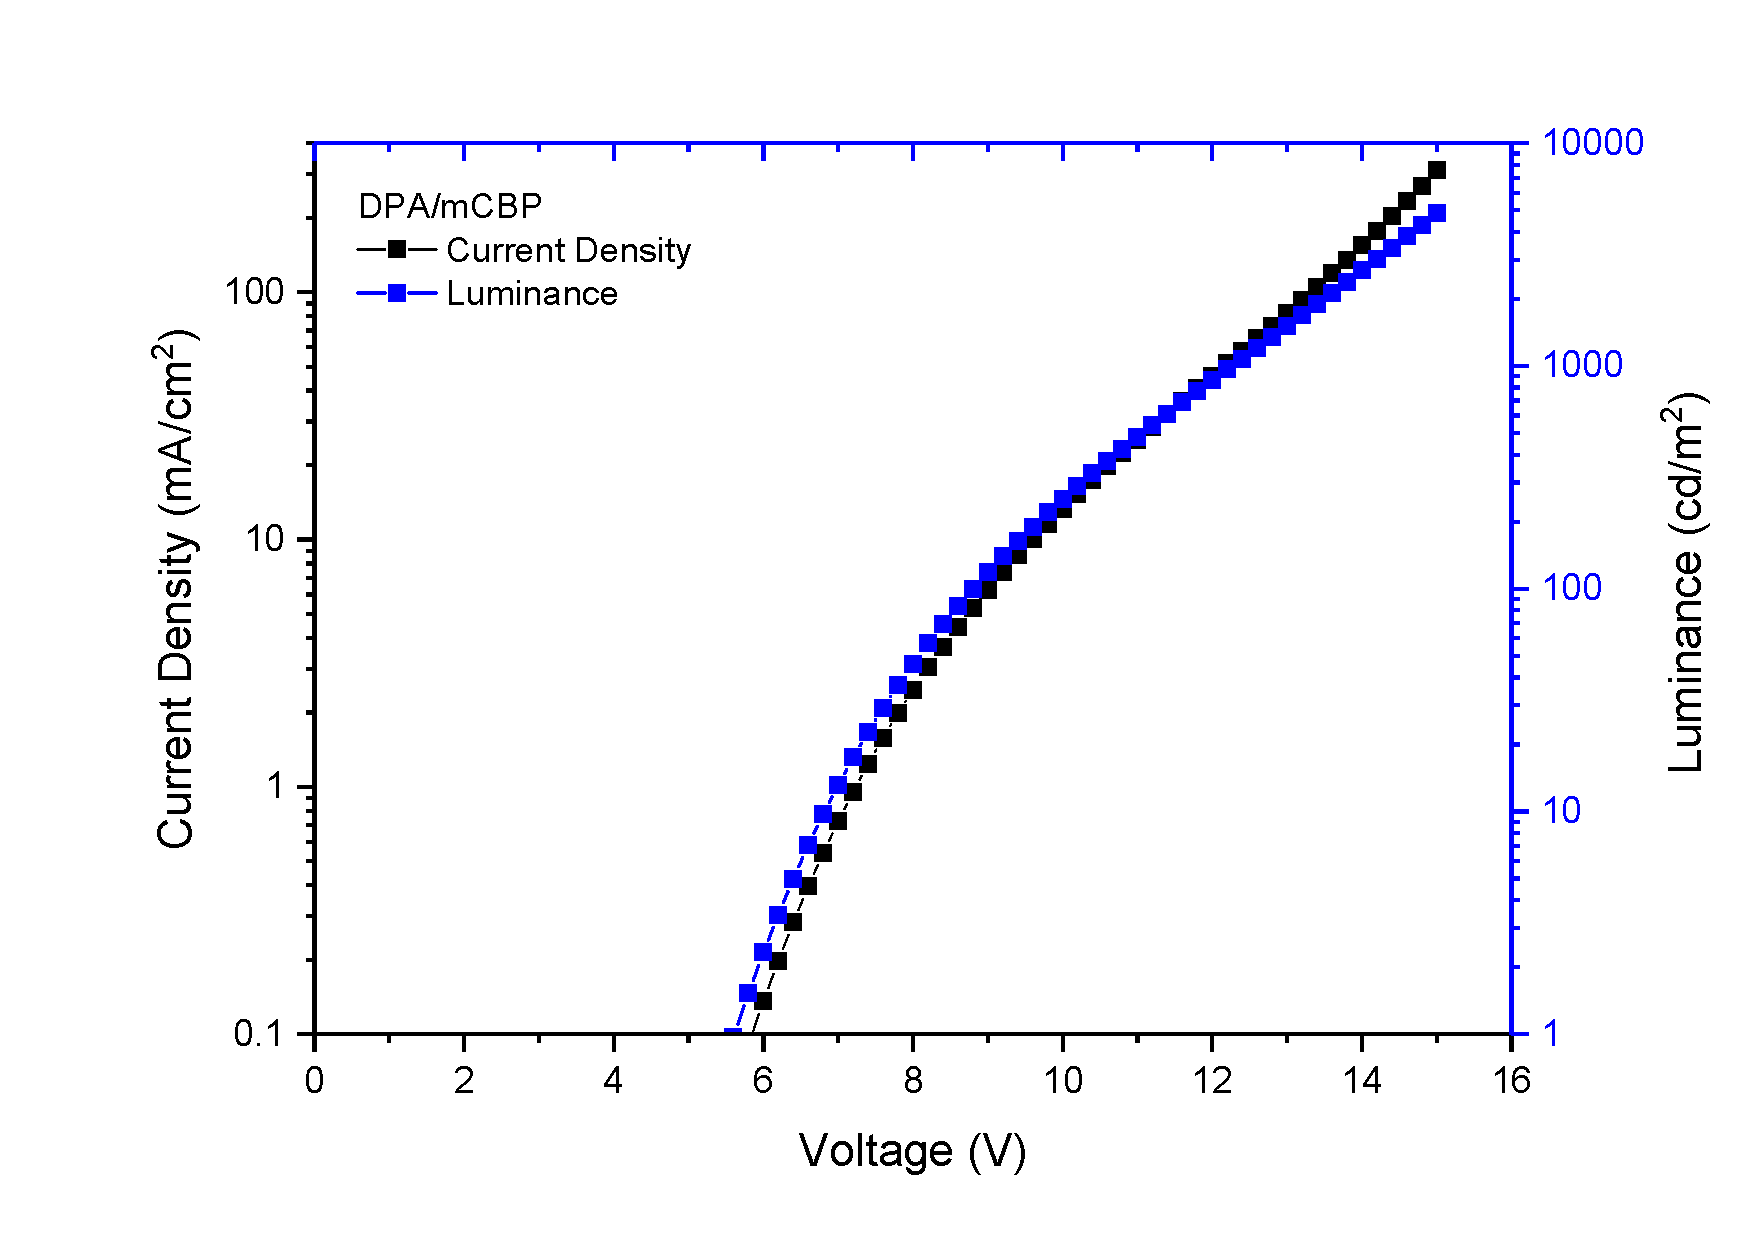
\includegraphics{./images/mCBPJVl.pdf}

}

\caption{\label{fig-mcbpkvl}Current density-luminance-voltage (J-V-L)
graph of doped 1wt\% 2,6-DPA/mCBP}

}

\end{minipage}%
%
\begin{minipage}[t]{0.50\linewidth}

{\centering 

\raisebox{-\height}{

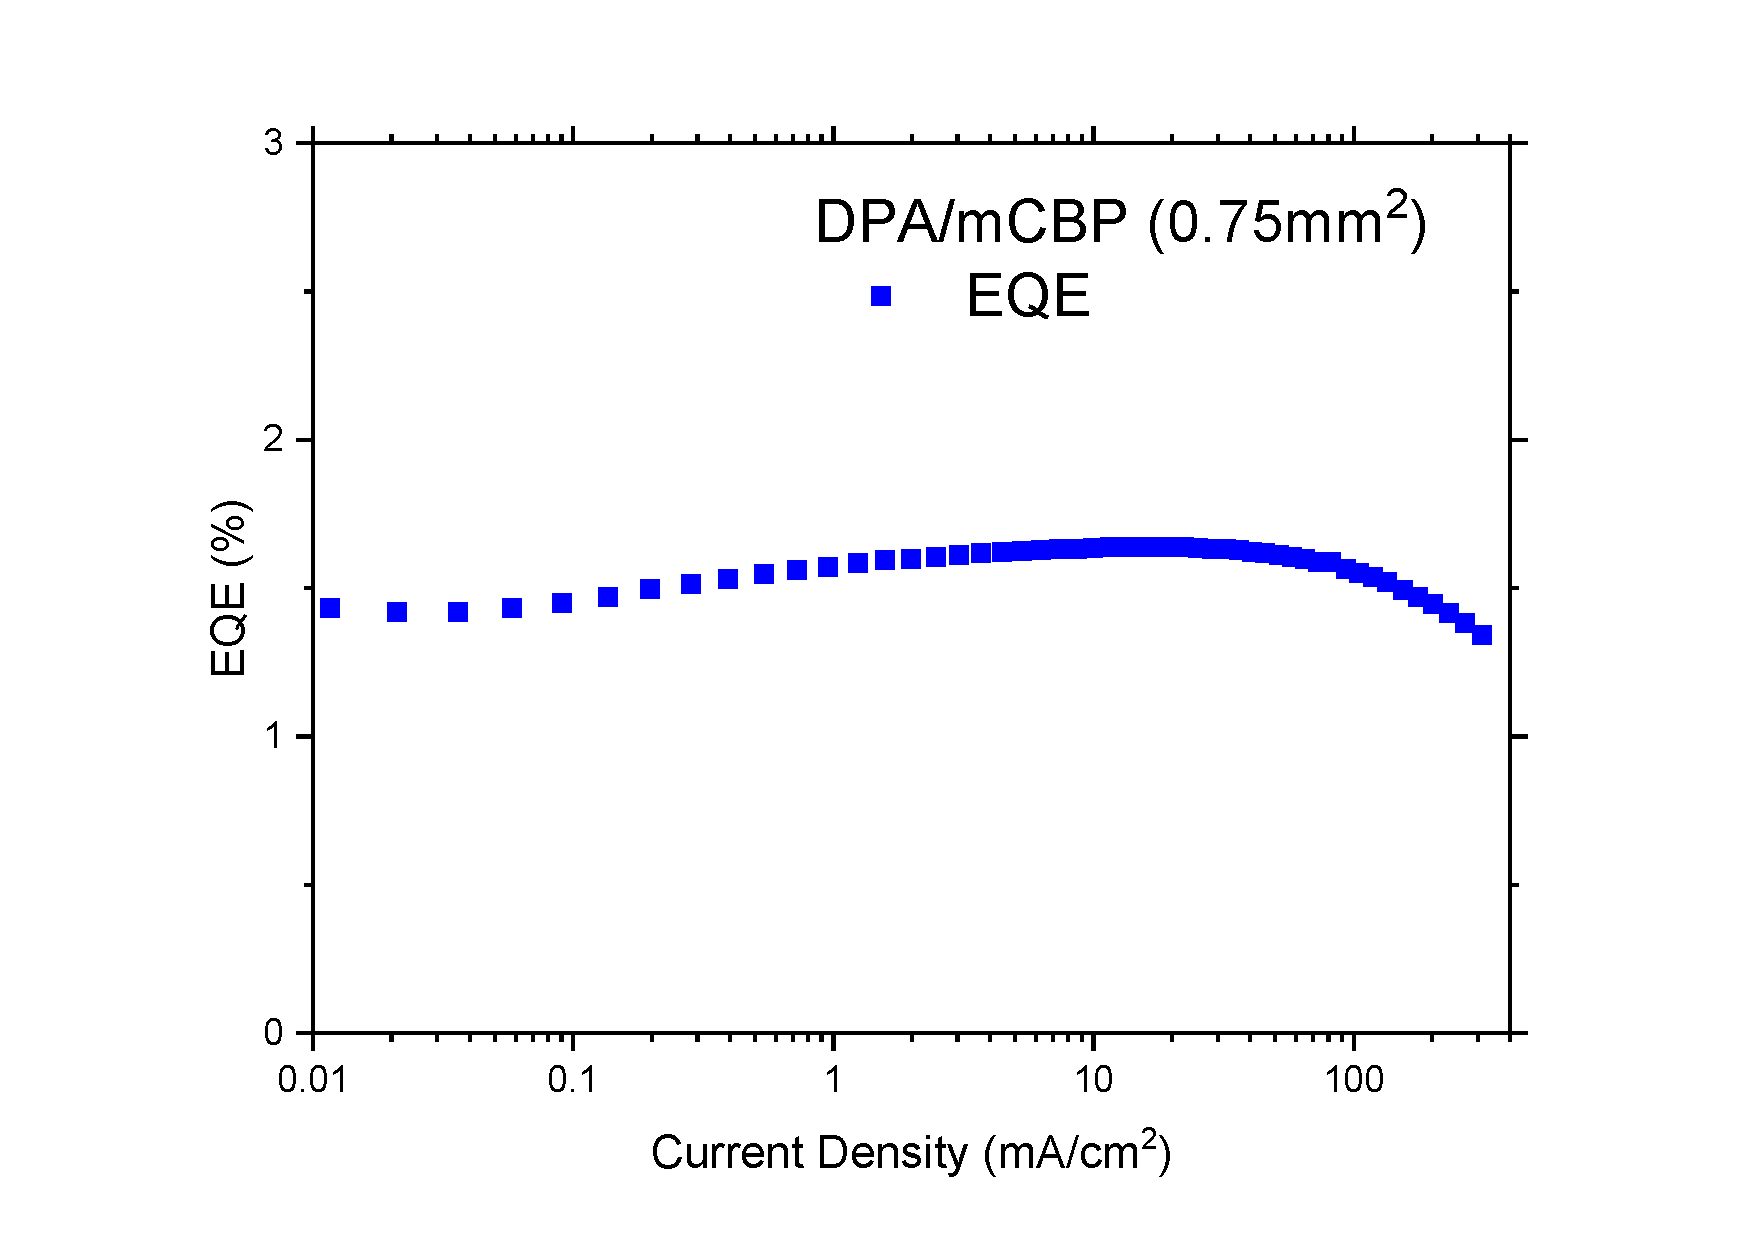
\includegraphics{./images/mCBPEQE.pdf}

}

\caption{\label{fig-mcbpeqe}EQE versus current density graph of doped
1wt\% 2,6-DPA/mCBP}

}

\end{minipage}%

\end{figure}

As mentioned in the introduction, in a current density versus luminance
plot (log-log scale) two regimes will appear with altering slopes. The
non-doped OLED demonstrates a clear regime change with a slope of
\(~1.7\pm0.05\) at low current densities, changing into
\(~0.74\pm0.03\). The transition current density is roughly
\(~20\pm10 mA/cm^2\). The slope is \(<2\) due to imperfect TTU and
losses, such as STA and other quenching. An observed slope shift from
\(>1\) to \(<1\) indicates definite gain of triplet to singlet excitons.

\begin{figure}

\begin{minipage}[t]{0.50\linewidth}

{\centering 

\raisebox{-\height}{

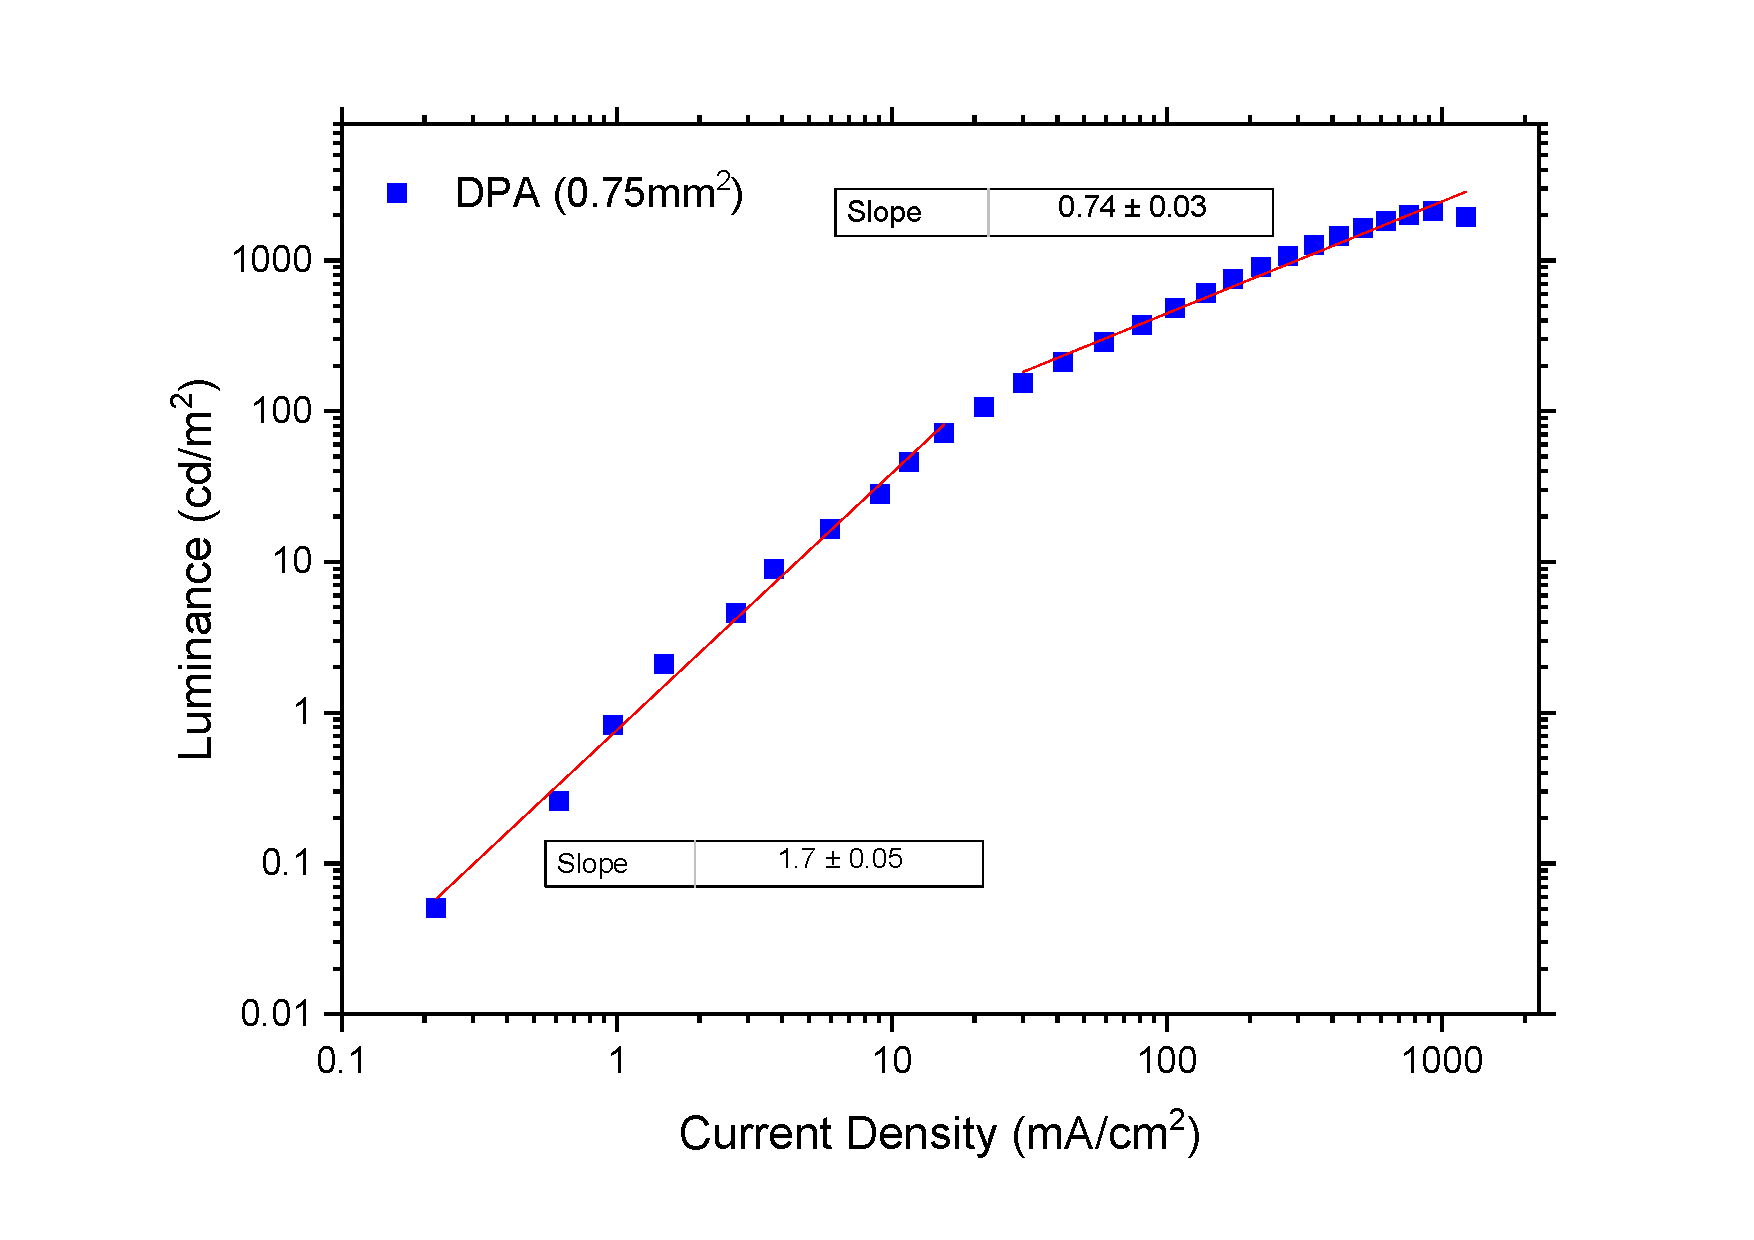
\includegraphics{./images/DpAAfit.pdf}

}

\caption{\label{fig-dpafit}Log-log scale Luminance versus current
density graph for OLEDs based on non-doped 2,6-DPA emissive layers}

}

\end{minipage}%
%
\begin{minipage}[t]{0.50\linewidth}

{\centering 

\raisebox{-\height}{

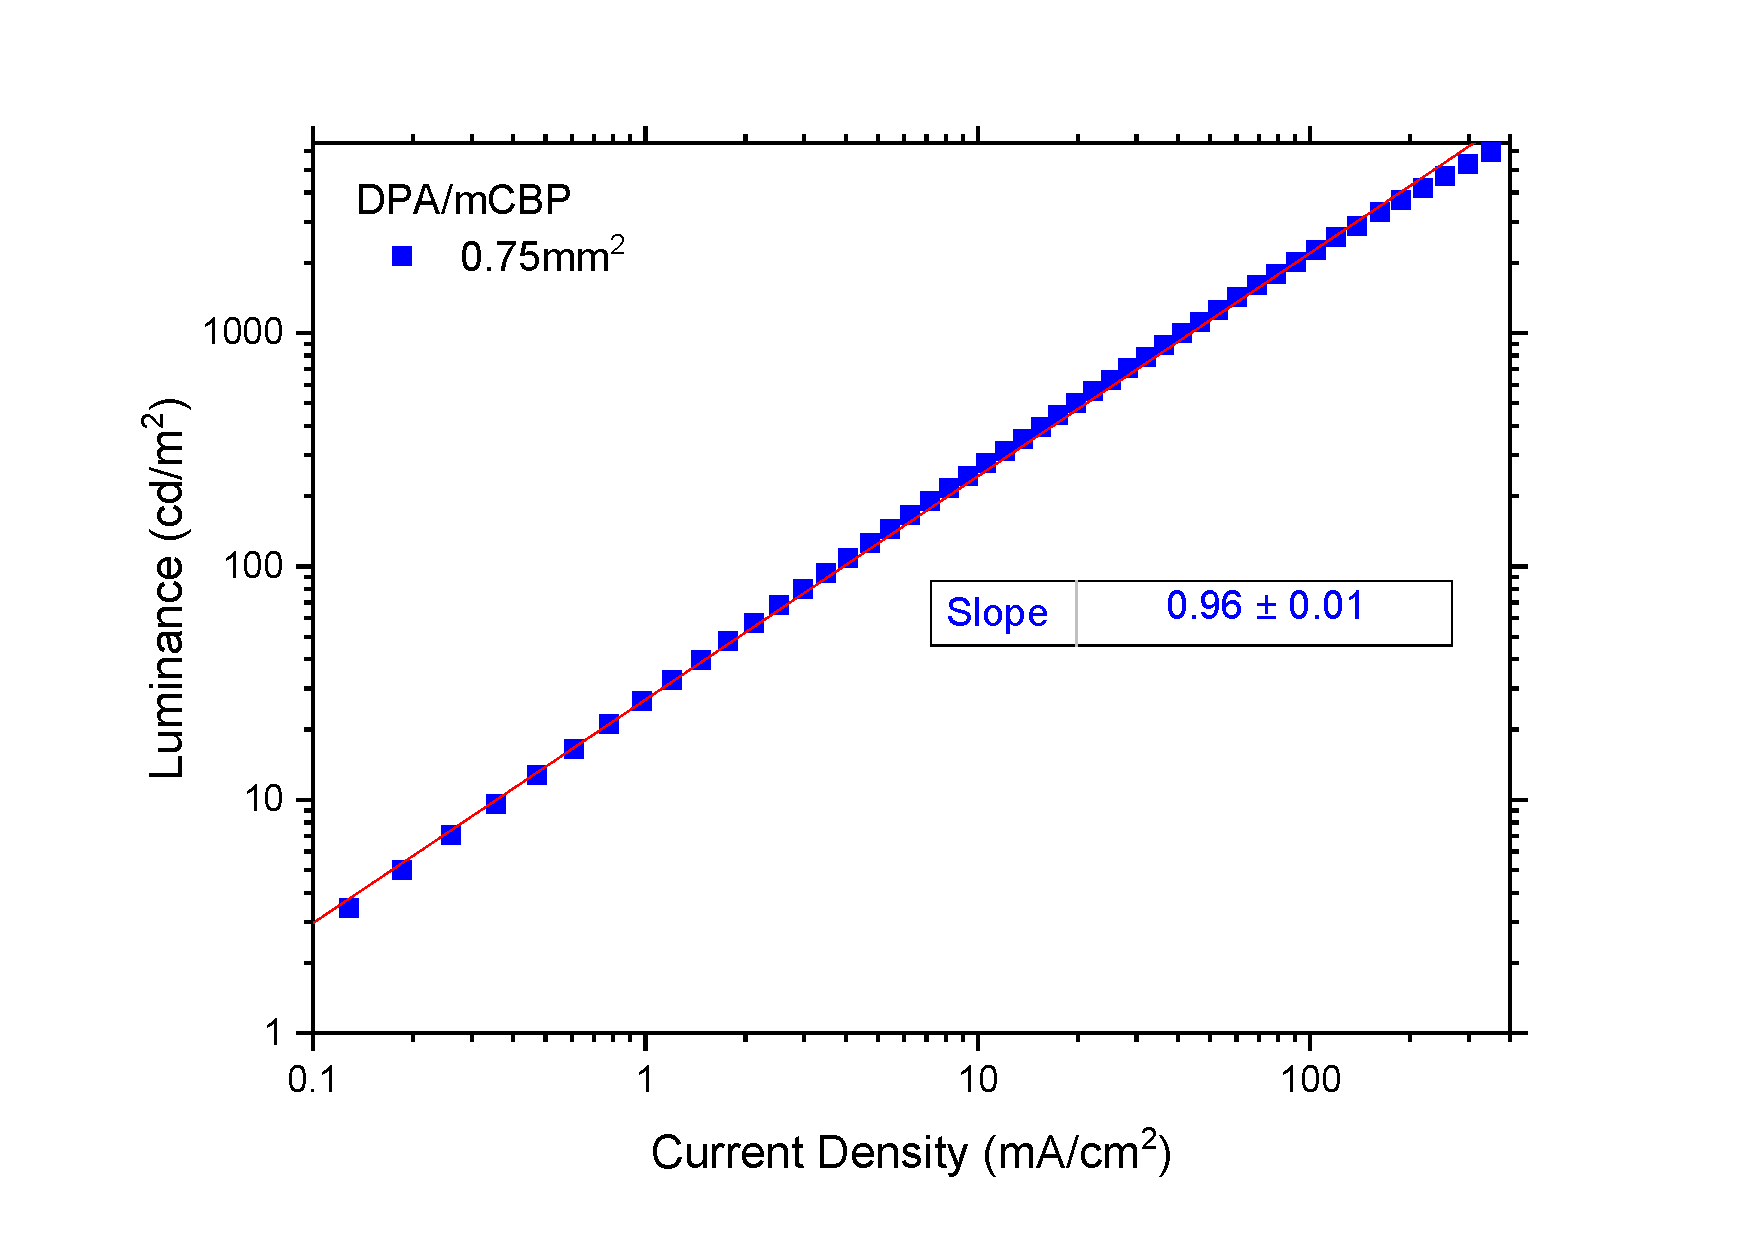
\includegraphics{./images/mCBPfit.pdf}

}

\caption{\label{fig-mcbpfit}Log-Log scale J-V-L for doped 2,6-DPA
emissive layers}

}

\end{minipage}%

\end{figure}

Pulse measurements (transient electroluminescence) will demonstrate the
population dynamics of the excitons even to high current densities. For
the non-doped film, 300 ns pulse widths were used to suppress Joule
heating while maintaining long enough steady-state lifetime to see the
gradual EL increase from TTU. The device area used was \(0.7mm^2\) to
reduce geometrical capacitance that minimises RC response distortion.
For doped films, a long pulse width (\(1.5\mu s\)) was used to
extrapolate the affect STA had on fluorescent materials at high current
densities. Whilst DC measurements only reached current densities of
\(1 A/cm^2\), pulse measurements reach densities of \(>2.5 A/cm^2\). At
high current densities, doped and non-doped devices show a sharp rise,
characteristic of space charge limited current conditions), with the
initial rise lifetime of \(~30 ns\). Non-doped devices at a lower
current density sees a longer initial rise (\(100ns\) at \(10 V\))
followed by a gradual increase as time progresses. This is
characteristic of TTU devices because of the recycling nature of the
triplet excitons generating additional singlets. At high current
densities (40 V) the steady state shows a slight decrease, indicating
STA has dominated rate over the TTU generation rate. How STA affects the
steady state in non-TTU devices can be seen in doped-devices (see
Figure~\ref{fig-mcbppulse}\}) -- a noticeable decrease in EL as time
progresses. There is a \(~12\%\) difference between the steady states at
higher and lower current densities. At lower current densities, STA is
not prevalent so a steady state is visible. STA dominates via FRET, a
process that is determined by the spectral overlap between \(S_1\)
emission aand \(T_1\rightarrow T_n\) absorption bands.

\begin{figure}

\begin{minipage}[t]{0.50\linewidth}

{\centering 

\raisebox{-\height}{

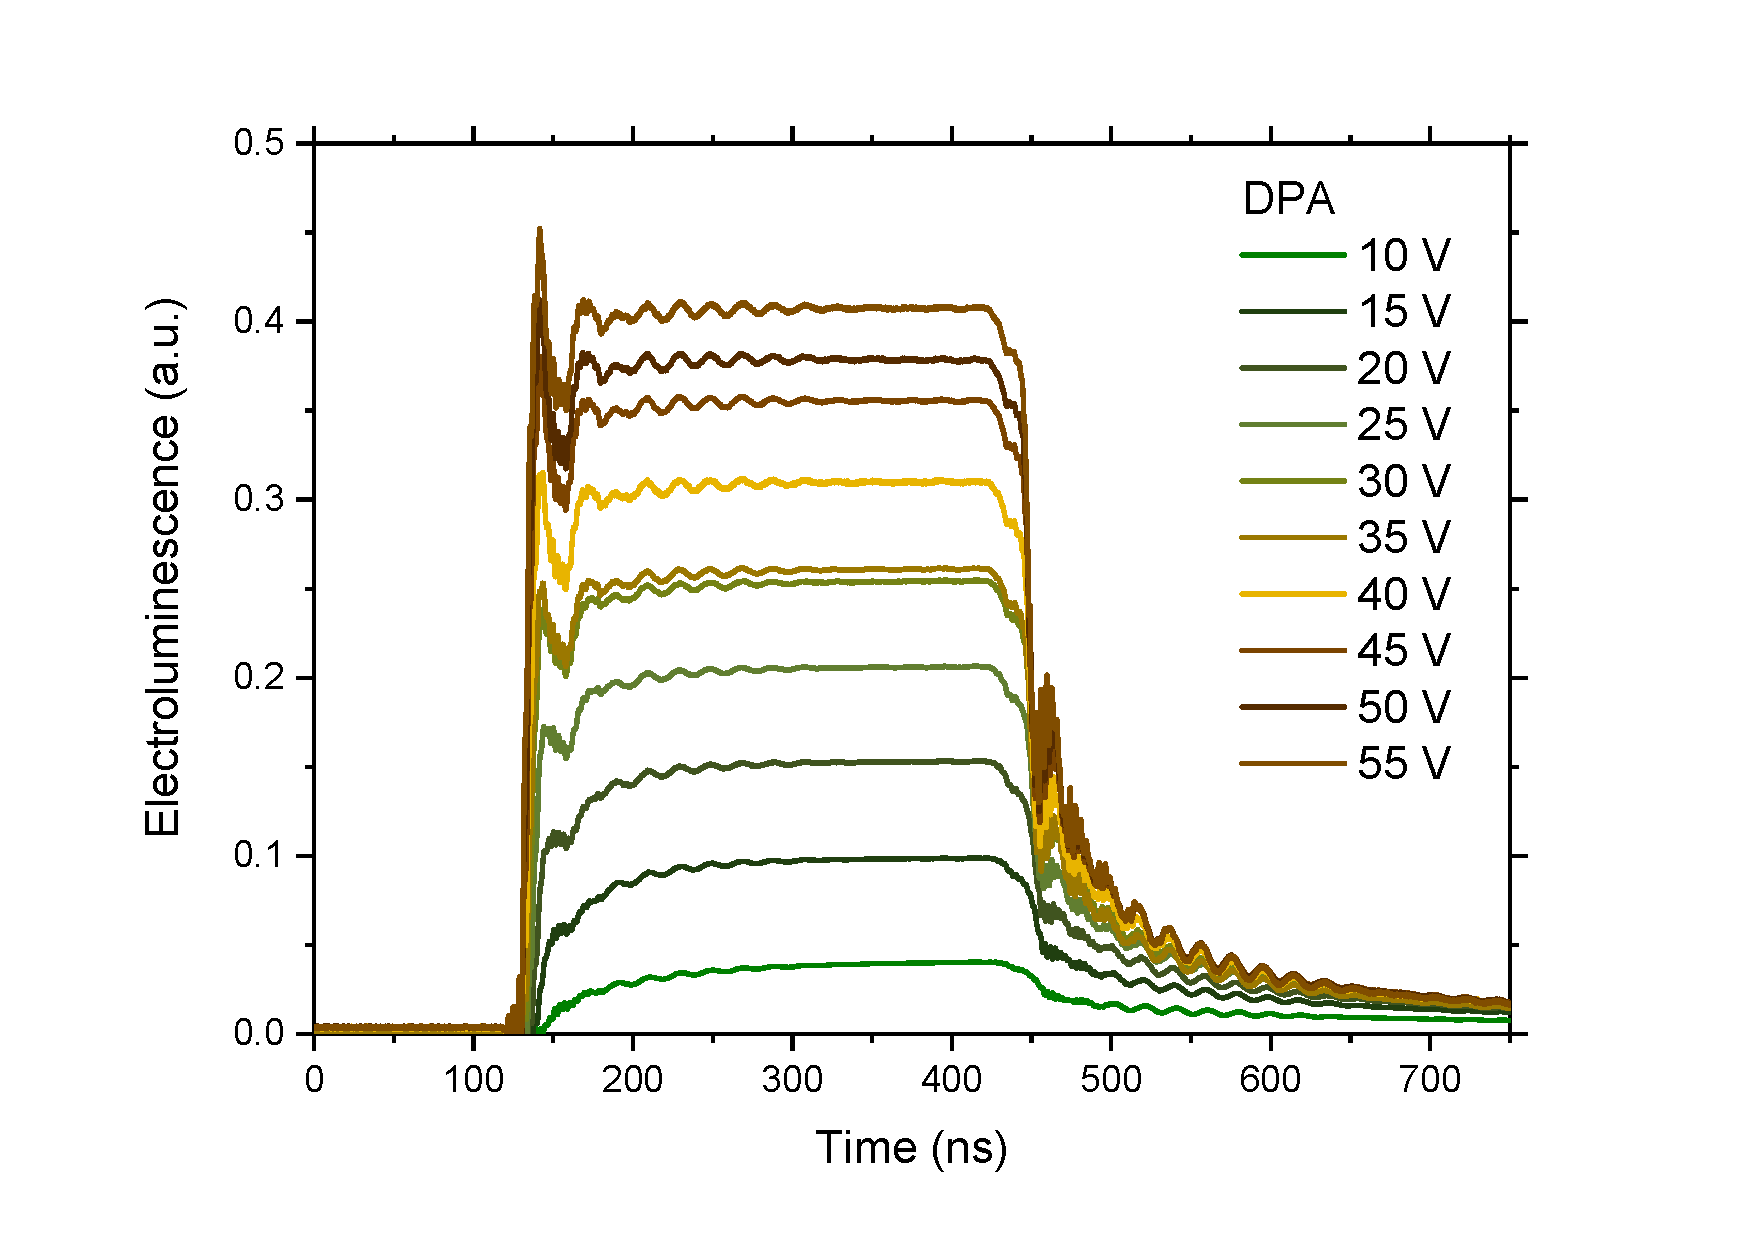
\includegraphics{./images/DPApulse.pdf}

}

}

\subcaption{\label{fig-dpapulse}}
\end{minipage}%
%
\begin{minipage}[t]{0.50\linewidth}

{\centering 

\raisebox{-\height}{

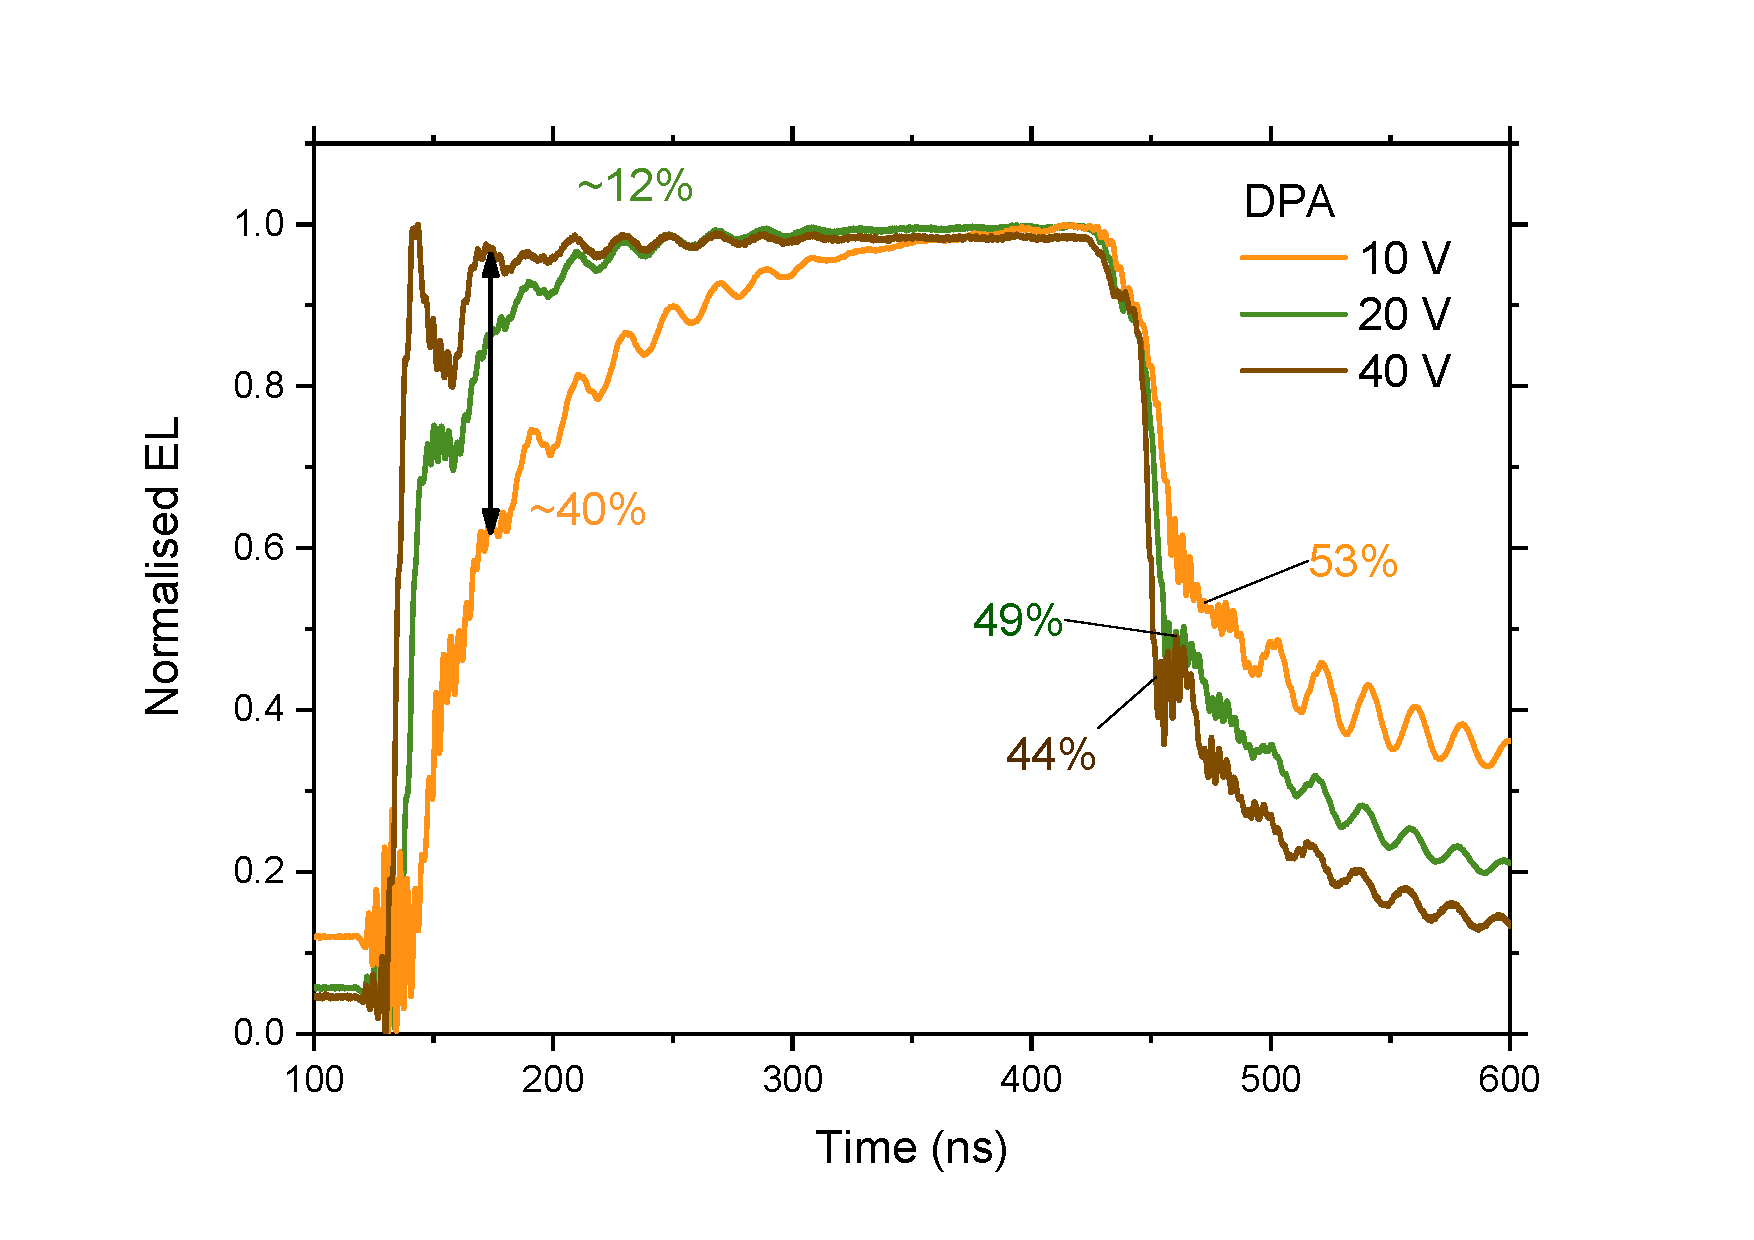
\includegraphics{./images/DPApulsezoom.pdf}

}

}

\subcaption{\label{fig-dpapzoom}}
\end{minipage}%
\newline
\begin{minipage}[t]{0.50\linewidth}

{\centering 

\raisebox{-\height}{

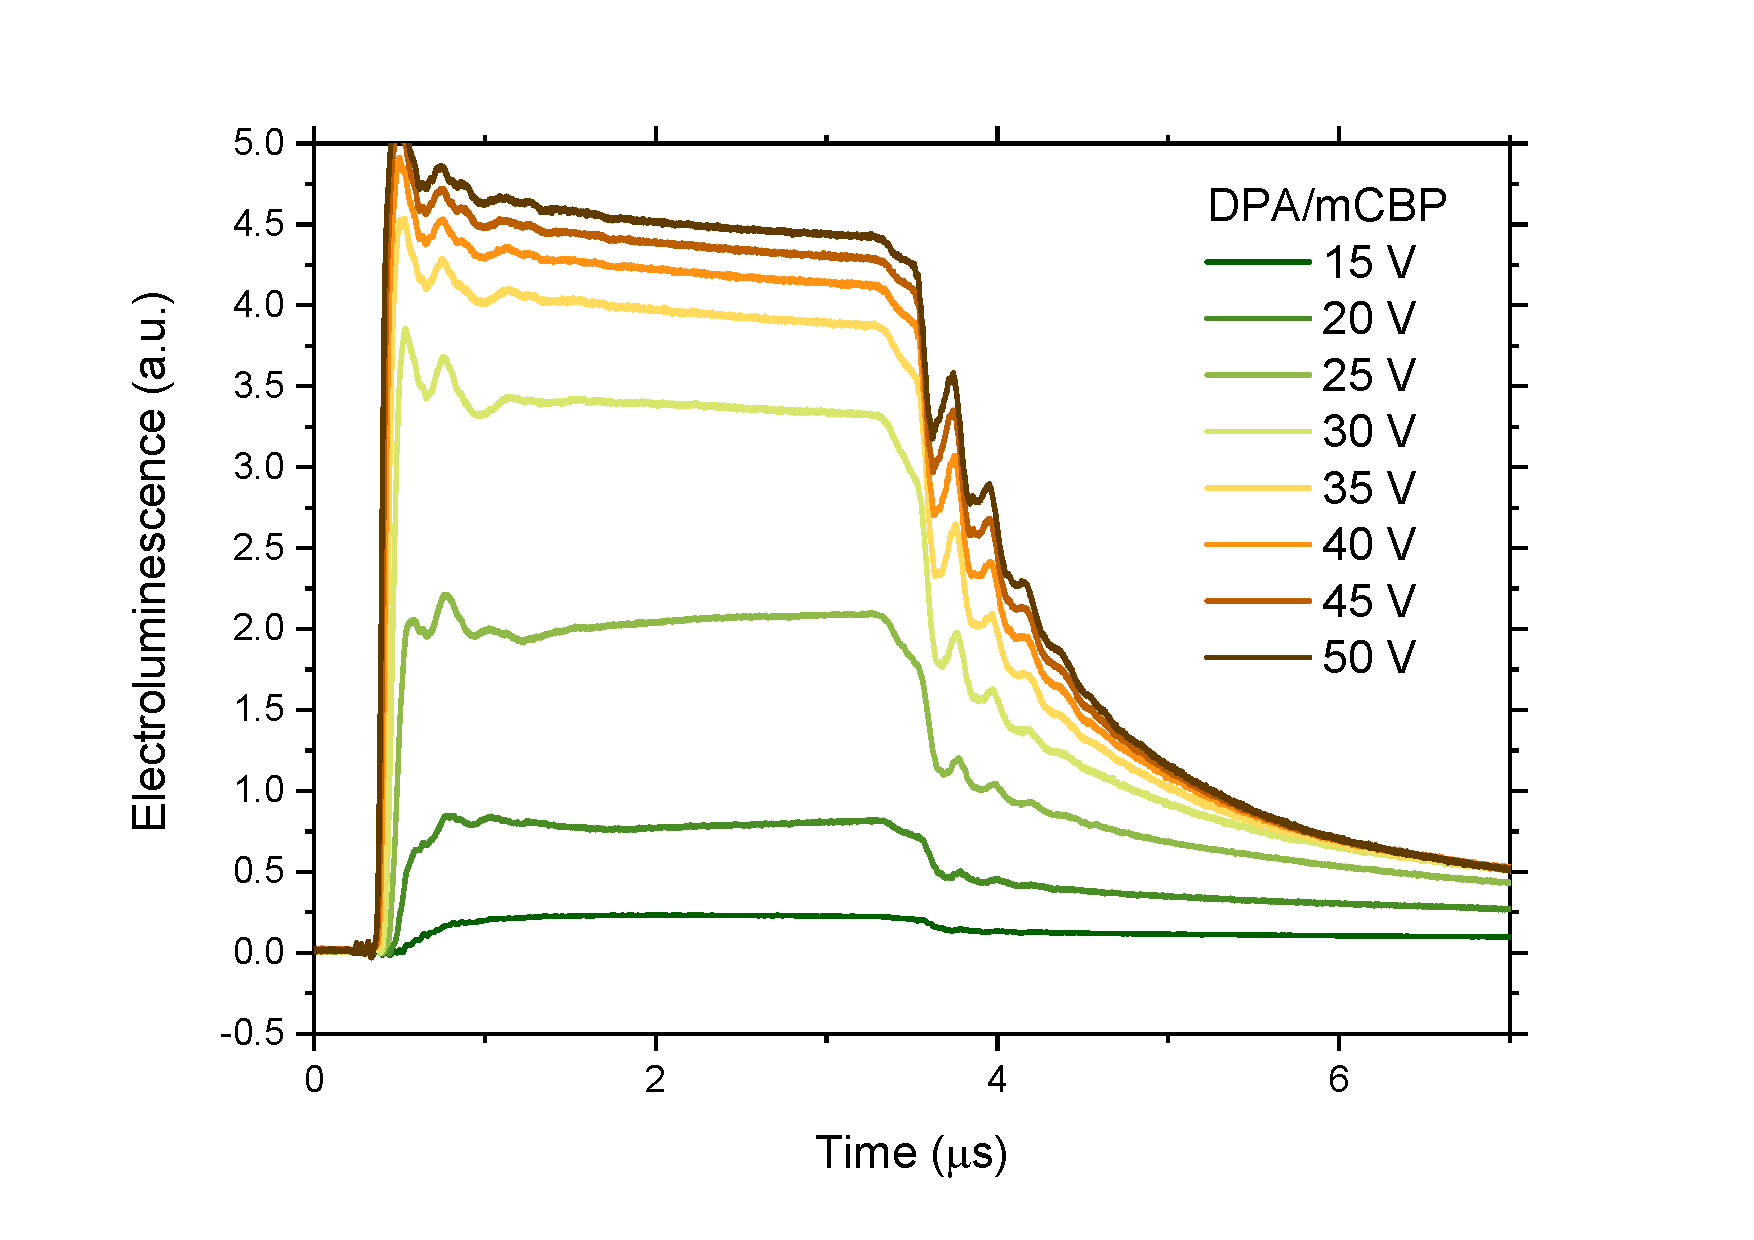
\includegraphics{./images/mCBPpulse.pdf}

}

}

\subcaption{\label{fig-mcbppulse}}
\end{minipage}%
%
\begin{minipage}[t]{0.50\linewidth}

{\centering 

\raisebox{-\height}{

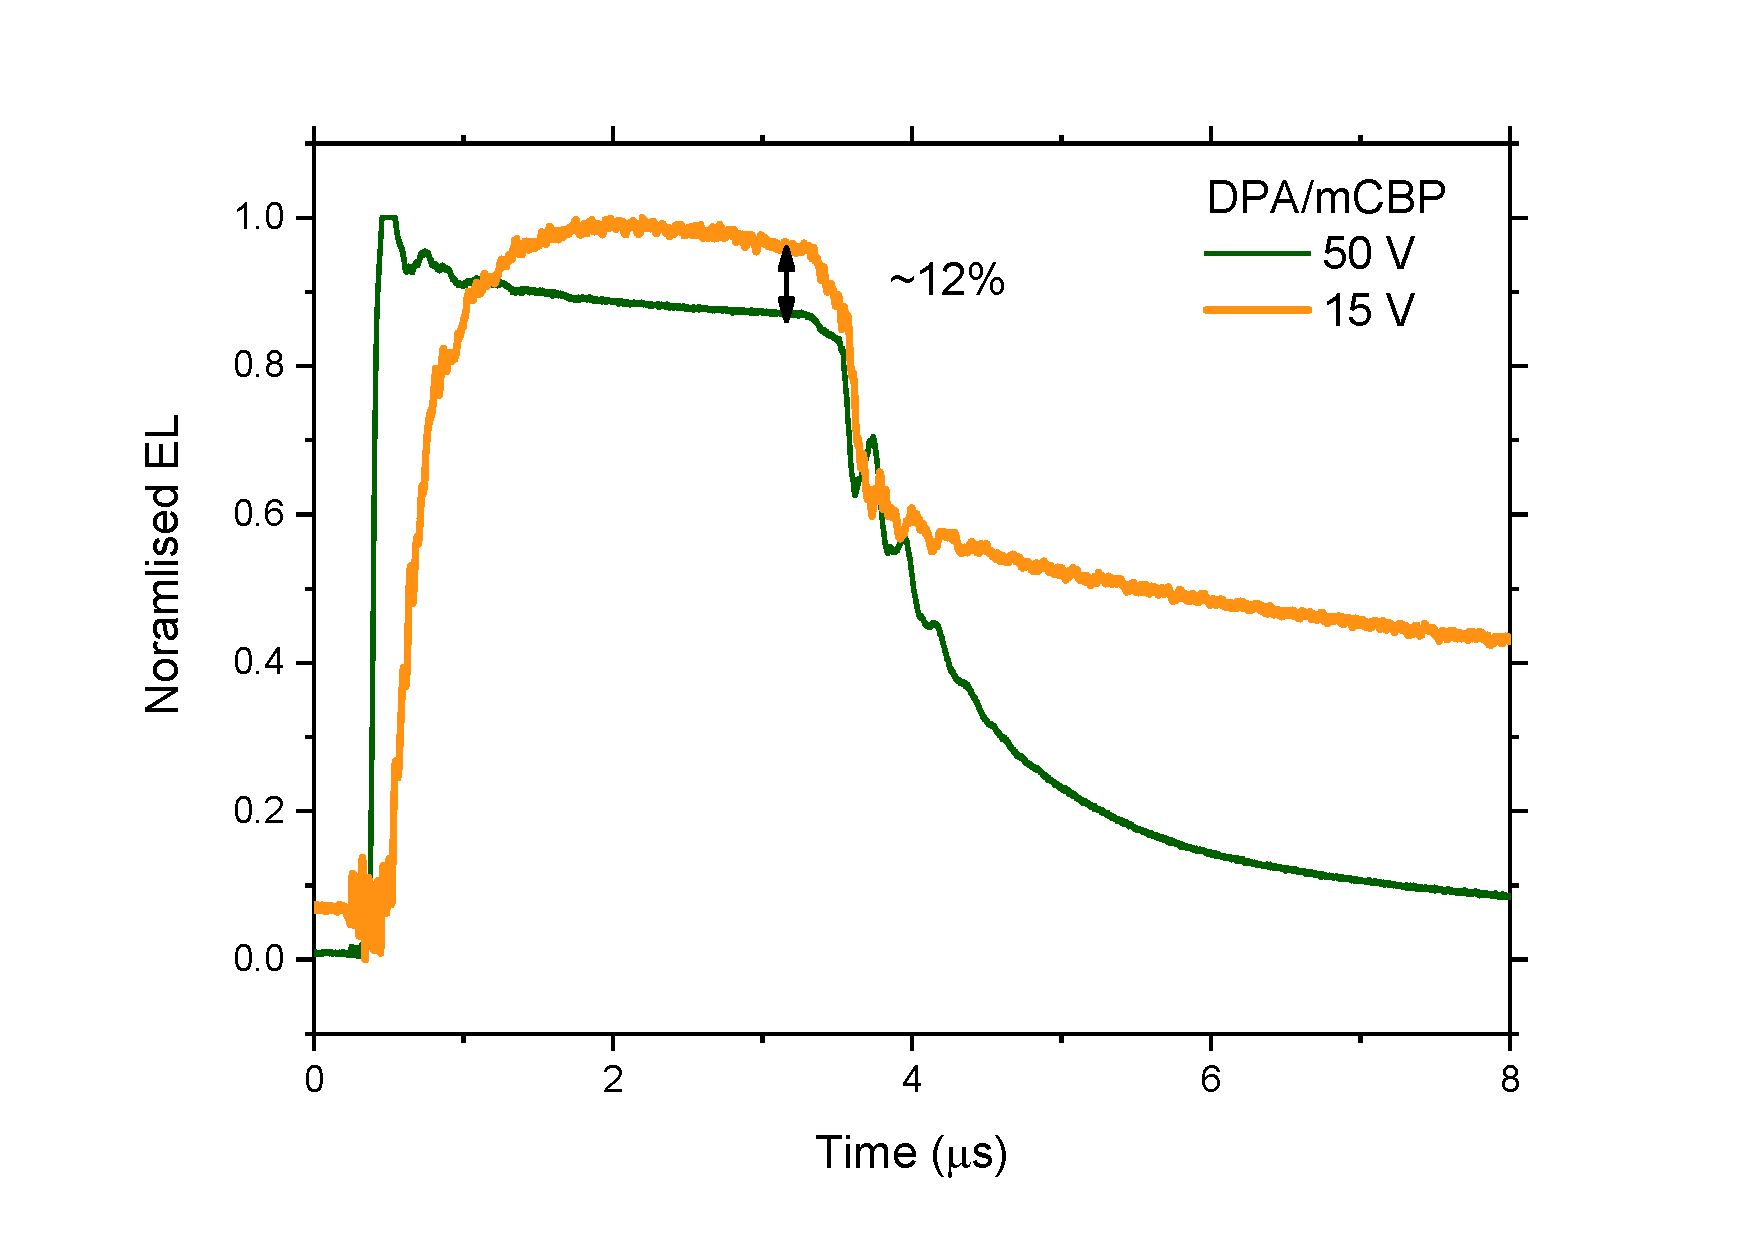
\includegraphics{./images/mCBPpulsezoom.pdf}

}

}

\subcaption{\label{fig-mcbppzoom}}
\end{minipage}%

\caption{\label{fig-pulse}Transient EL spectra of non-doped (a) for a
300 ns pulse width and doped (c) for 1.5{μs} across many voltages. The
comparison of steady state growth at low current densities versus high
current densities are shown in (b) and (d), as well as the delayed
components}

\end{figure}

The turn off electroluminescence of pulse measurements also provide
useful information. For TTU devices, a prompt decay is expected after
voltage turn off due to the loss of direct singlet generation, followed
by a delayed fluorescence (DF) bimolecular decay function
\[EL_{DF} = \frac{1}{(a+bt)^2}\] where \(a\) and \(b\) are constants.
Trapped carriers recombining will cause a delayed fluorescence component
with slope between close to 1 (Debye and Edwards 1952; Kabe and Adachi
2017), as we see in Figure~\ref{fig-mcbpfit}.

\begin{figure}

\begin{minipage}[t]{0.50\linewidth}

{\centering 

\raisebox{-\height}{

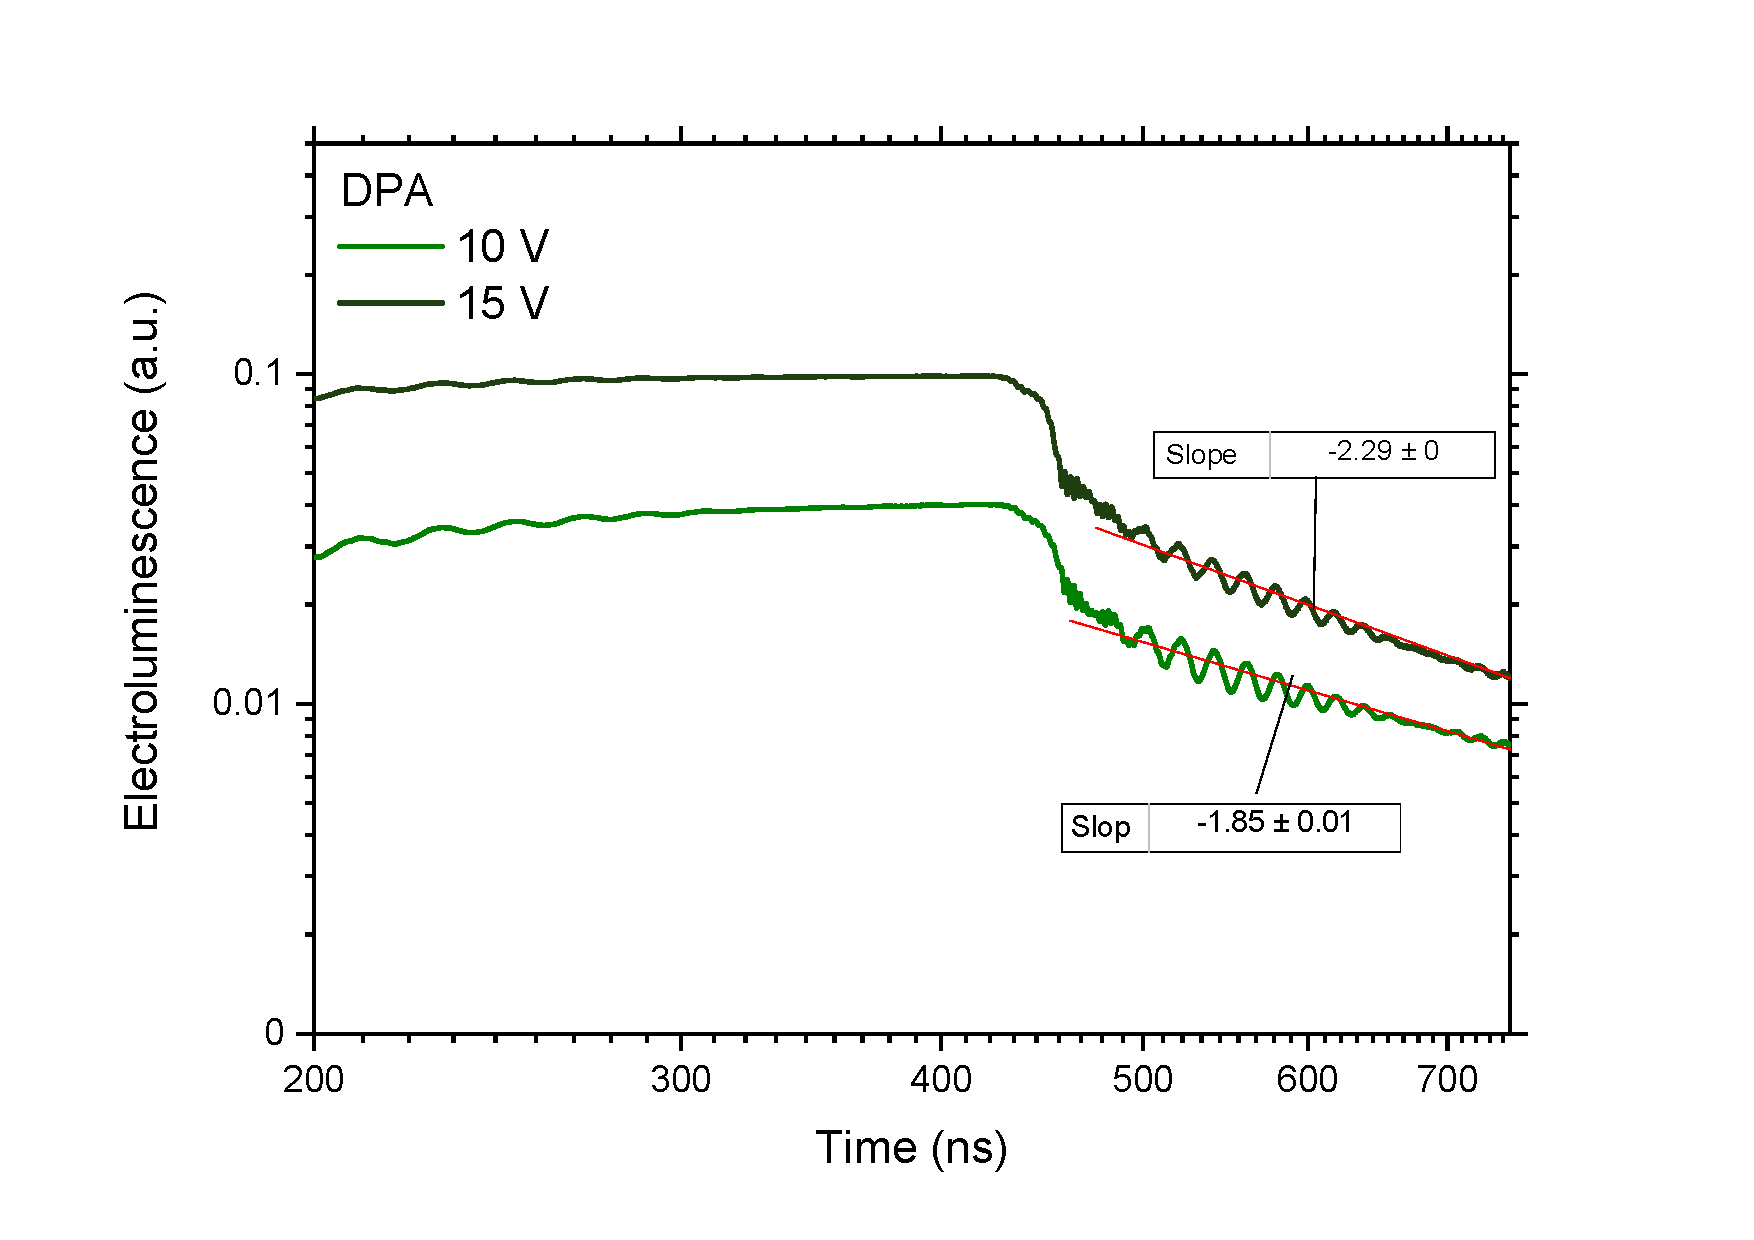
\includegraphics{./images/DPAslopefit.pdf}

}

}

\subcaption{\label{fig-dpaslopefit}}
\end{minipage}%
%
\begin{minipage}[t]{0.50\linewidth}

{\centering 

\raisebox{-\height}{

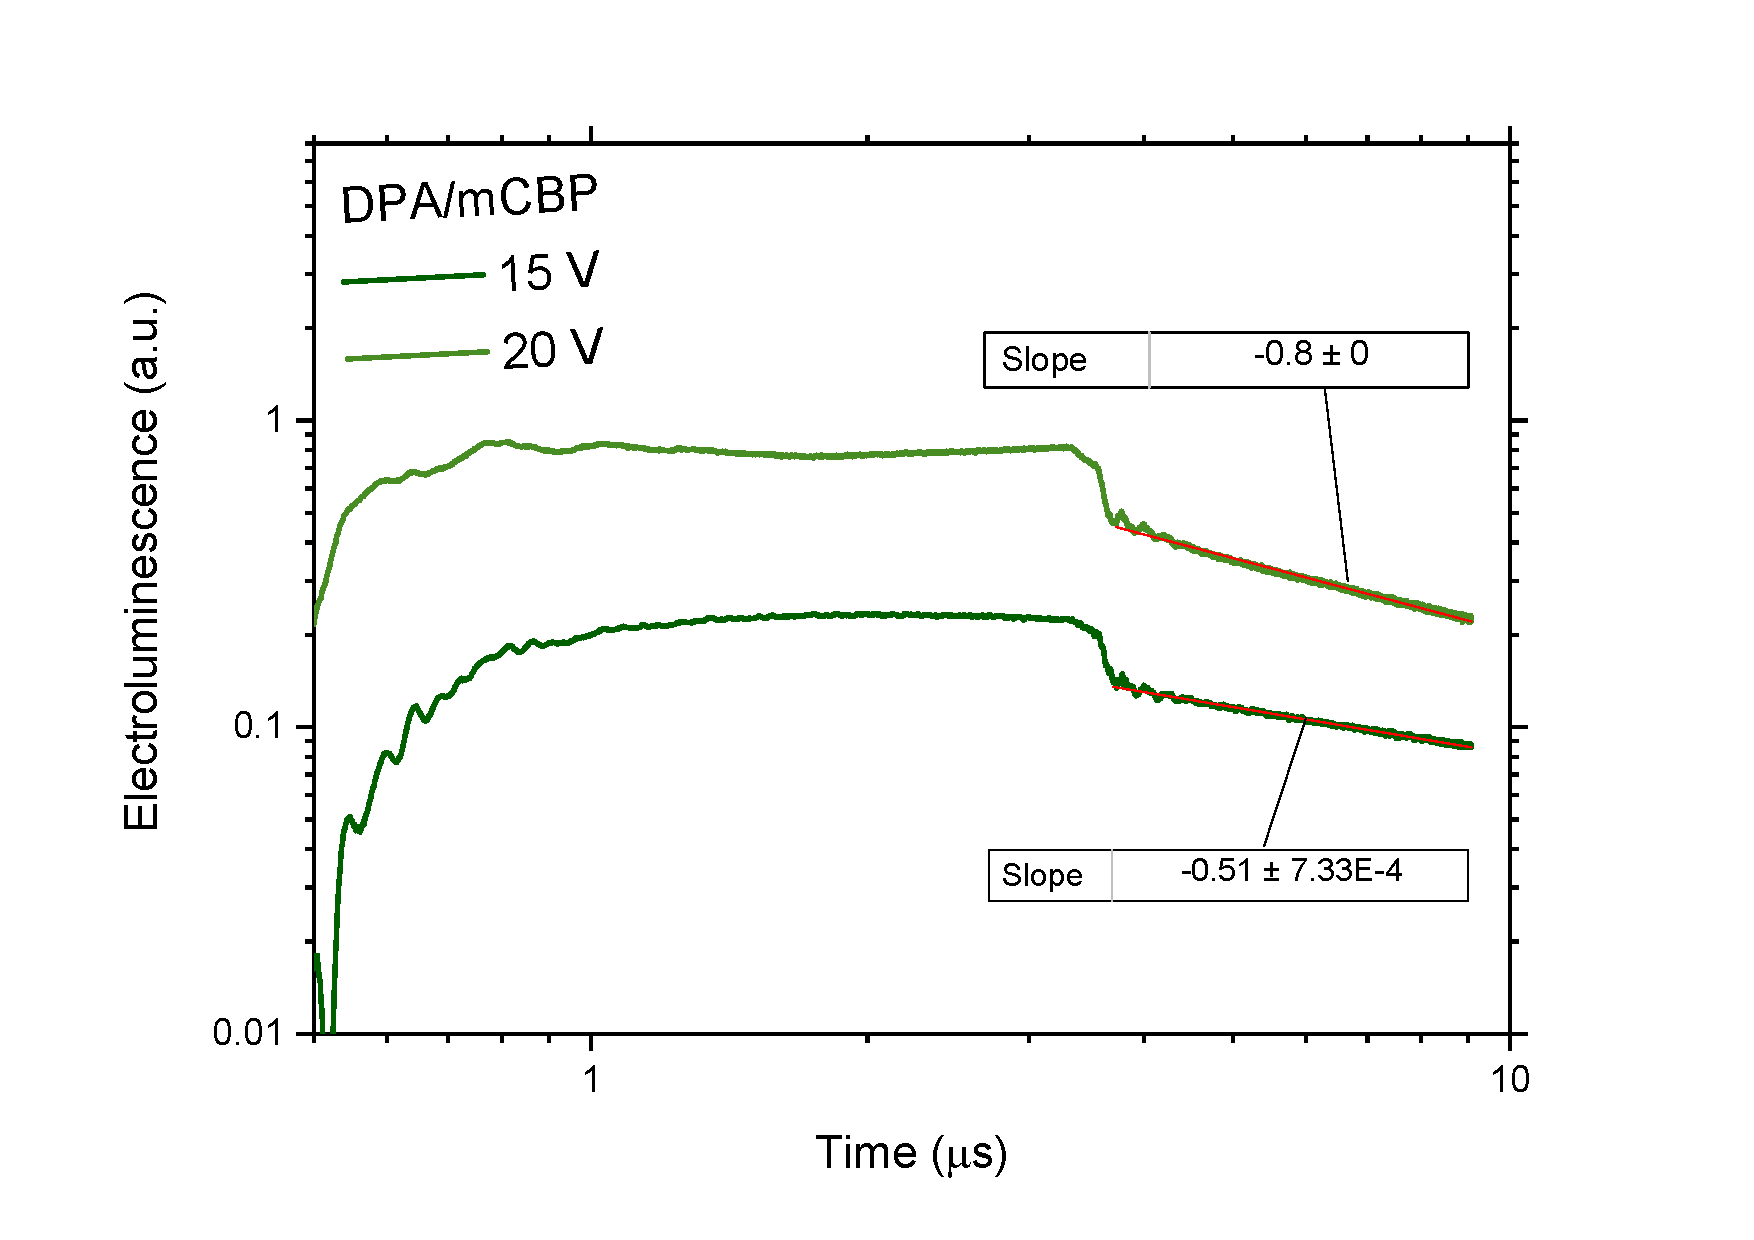
\includegraphics{./images/mCBP slope fit.pdf}

}

}

\subcaption{\label{fig-mcbpfit}}
\end{minipage}%

\caption{\label{fig-slopefit}Log-Log scale transient EL spectra of
non-doped (a) for a 300 ns pulse width and doped (b) for 1.5{μs} at 10
at 20 V. The delayed component has a slope of ~2 matching TTU
contribution.}

\end{figure}

\hypertarget{discussion}{%
\section{Discussion}\label{discussion}}

\begin{figure}

{\centering 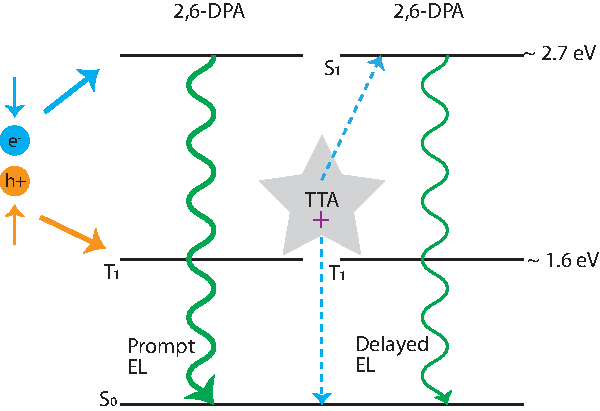
\includegraphics{./images/TTA in DPA.pdf}

}

\caption{\label{fig-ttadpa}The triplet-triplet annihilation upconversion
process in 2,6-DPA. The singlet {S1} and triplet {T1} energy levels are
shown, where {S1 \textless{} 2T1}.\textless/}

\end{figure}

2,6-DPA is an anthracene derivative with low PLQY and moderate charge
mobility in amorphous state. In neat film OLEDs, 2,6-DPA shows
distinctive TTU properties such as distinctive regimes in the J-L
log-log plot, with a TTU threshold of \(~20\pm10 mA/cm^2\). Not only
does it exhibit steady state increase at low current densities, showing
a \(40\%\) rise over \(~300ns\) pulse width, but it also exhibits a
delayed fluorescence component following the triplet-triplet
upconversion DF trend. The TTU process in neat films can be seen in
Figure~\ref{fig-ttadpa}. This 2,6-DPA neat film was compared to the
doped film 2,6-DPA in \(10wt\%\) mCBP, which was created to separate the
chromophores of 2,6-DPA to extend the triplet states beyond the
short-range Dexter energy transfer process. This was successful as the
doped OLED showed trends of typical fluorescence. Despite the peak EQE
not surpassing the theoretical maximum of typical fluorescent emitters
-- a feat that would confirm extra exciton generation -- the evidence
presented here is enough to show 2,6-DPA shows promise for enhancing a
host-guest system with TTU. To increase device performance, optimisation
of fabrication process and device structure needs to be considered
specific to an amorphous 2,6-DPA film.

\bookmarksetup{startatroot}

\hypertarget{sec-c6}{%
\chapter{TTU in a Host-Guest system to enhance Coumarin6}\label{sec-c6}}

\hypertarget{introduction-1}{%
\section{Introduction}\label{introduction-1}}

In this section, I preliminary investigated the electroluminescence
properties of a model anthracene derivative 2,6-diphenylanthracene
(2,6-DPA) (J. Liu, Zhang, et al. 2015; J. Liu, Dong, et al. 2015) doped
in a known lasing material,
3-(2-Benzothiazolyl)-N,N-diethylumbelliferylamine (Coumarin6) (C. W.
Tang, VanSlyke, and Chen 1989; Kido and Iizumi 1998) at \(~1-2wt\%\).
Coumarin caan be confied between the large singlet-triplet energy level
gap of 2,6-DPA, which enables transfer of singlets to the guest, and
triplets from the guest to host for further TTU (see Figure
(\textbf{fig:ttucoumarin?})). The OLED structure can be found in
Appendix \protect\hyperlink{apen:oledex}{{[}apen:oledex{]}}.
2,6-DPA/Coumarin6 was based in OLEDs that were then tested and analysed
under steady state and microsecond pulse excitation. The low \(wt\%\) of
Coumarin6 guest is to avoid separation of the chromophores of 2,6-DPA.
That way the Dexter energy transfer of triplet-triplet annihilation can
happen frequently. A similar doping approach has been used to obtain
high EQEs due to TTU (Zhang and Forrest 2011), and reduce STA in
optically pumped lasers (J. U. Kim et al. 2020). Herein, I found that
2,6-DPA/Coumarin6 host/guest exhibits the TTU mechanism to generate
extra singlet excitons, yet does not achieve a better performance than
non-doped. At low-current densities (J) the EQE of the device increases
proportionally to \(J\) because of the absence of dominating
singlet-triplet annihilation (STA). At high current densities, STA
becomes a significant loss causing a reduction in EQE and gain. The
transition between the dominating regions of
\(T{transition}\>(k_{TTU}\tau)^-1\) and the inverse are clearly visible,
yet the transient electroluminescence does not demonstrate promising
results. Herein, I will explain the promise of these preliminary results
regarding TTU and coumarin6.

\begin{figure}

{\centering 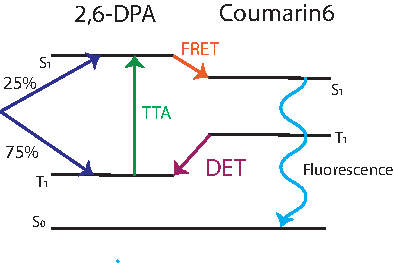
\includegraphics{./images/coumarinTTU.pdf}

}

\caption{\label{fig-ttucoumarin}The triplet-triplet annihilation
upconversion process in 2,6-DPA/Coumarin6 host-guest system. The singlet
{S1} and triplet {T1} energy levels are shown, where
{S1 \textless{} 2T1} for 2,6-DPA.}

\end{figure}

\hypertarget{results-1}{%
\subsection{Results}\label{results-1}}

The OLED devices that were creates followed the structure, Indium Tin
Oxide (ITO) 100nm /
N,N'-Di(1-naphthyl)-N,N'-diphenyl-(1,1'-biphenyl)-4,4'-diamine (NPB)
40nm / 2,6-DPA and Coumarin6 (~1-2wt\%) 40nm /
1,3,5-Tris(3-pyridyl-3-phenyl)benzene (TmPyPB) 30nm / Calcium 5nm /
Aluminum 100nm. Each layer was thermally evaporated under high vacuum
(\(10^-6 mbar)\) without break to avoid atmosphere exposure. The
deposition rate for the organic layers were between \(0.3 - 0.6 Å/s\).
To achieve \(~1-2wt\%\) , a simultaneous doping of coumarin6 and 2,6-DPA
deposition with rates \(0.01Å/s\) and \(1Å/s\) minimum was required. The
thermal evaporator's smallest deposition rate was \(0.01Å/s\) so this
become quite troublesome to manage. Exceeding \(1Å/s\) is not preferable
due to piercing of the beneath layer. The thickness and structure was
chosen as per the OLEDs made in the previous section to best compare
device performance difference. The spectra showed a pale green emission
(peak 520 nm).

\begin{figure}

\begin{minipage}[t]{0.50\linewidth}

{\centering 

\raisebox{-\height}{

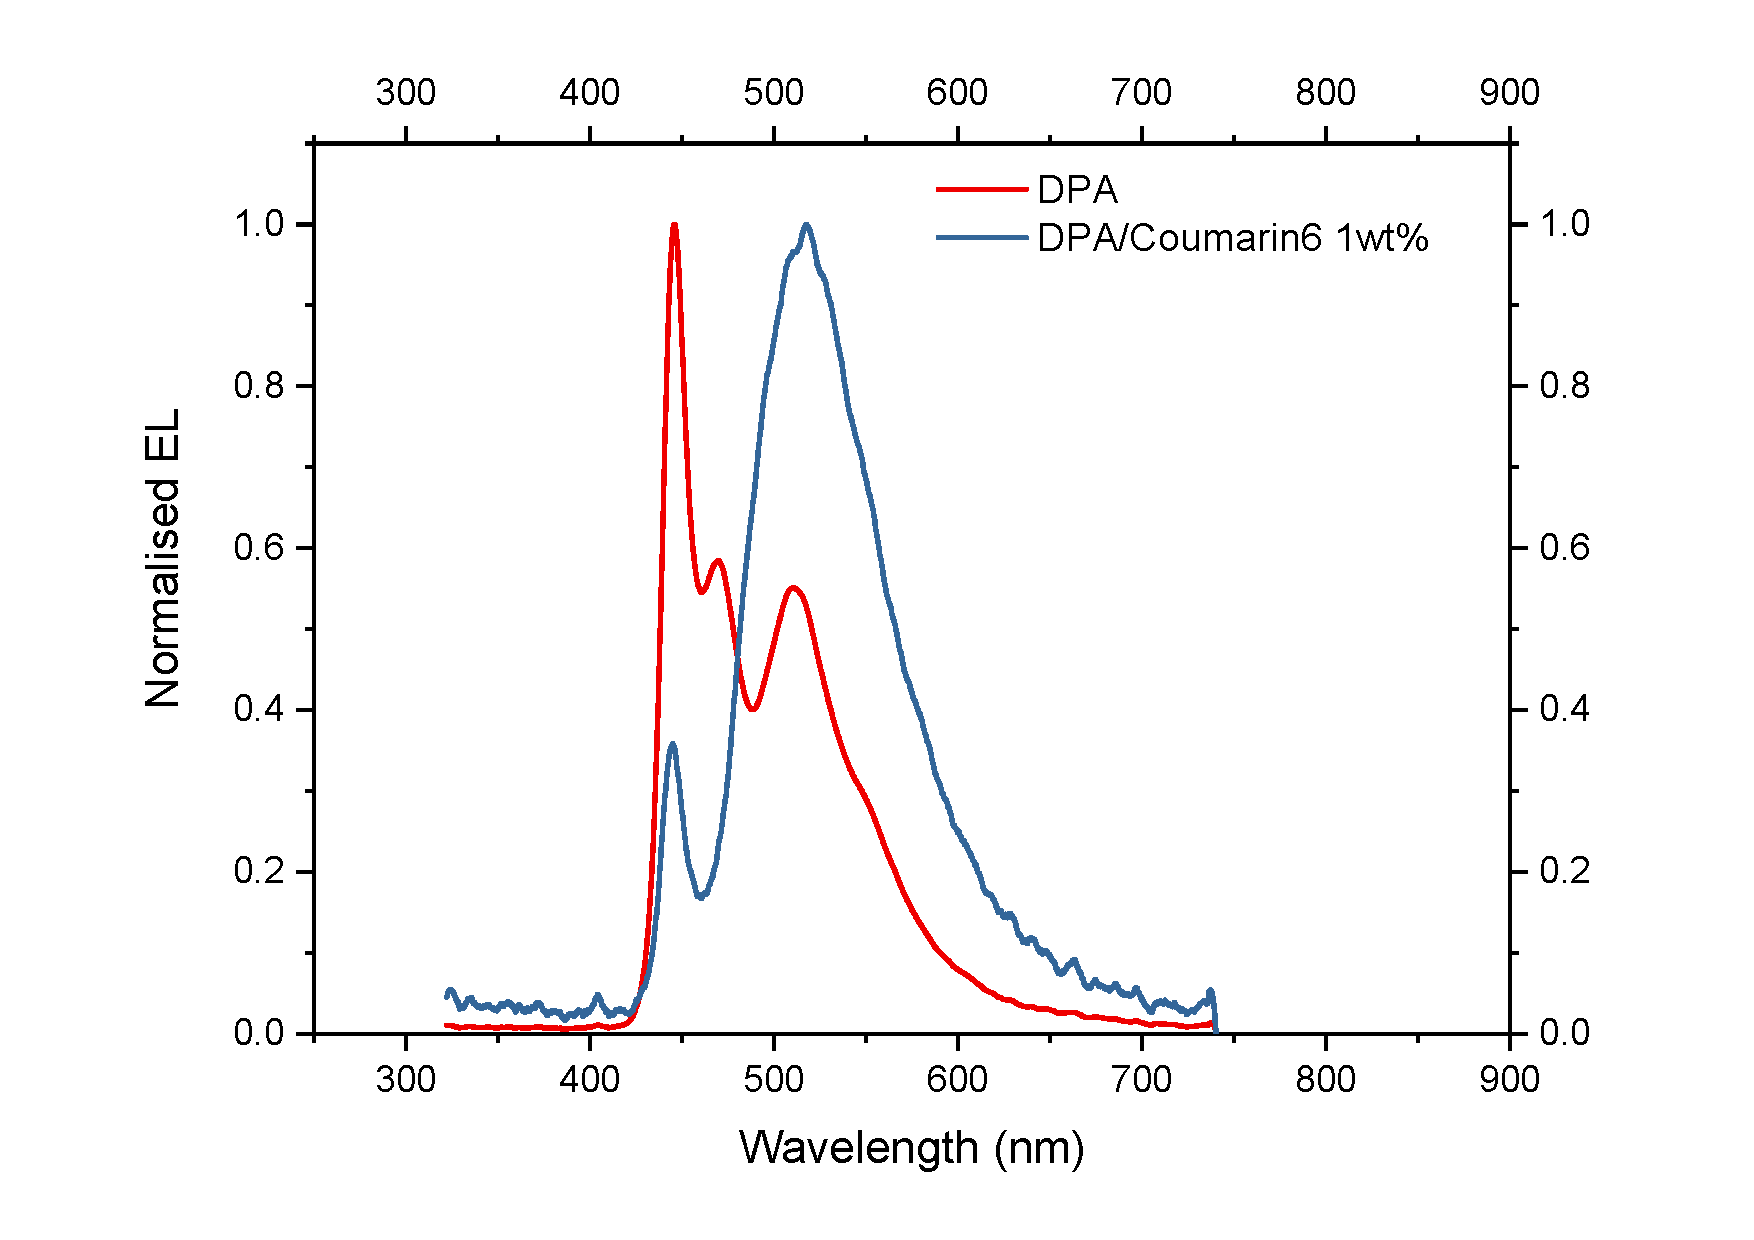
\includegraphics{./images/coumarinspectra.pdf}

}

}

\subcaption{\label{fig-cspectra}}
\end{minipage}%
%
\begin{minipage}[t]{0.50\linewidth}

{\centering 

\raisebox{-\height}{

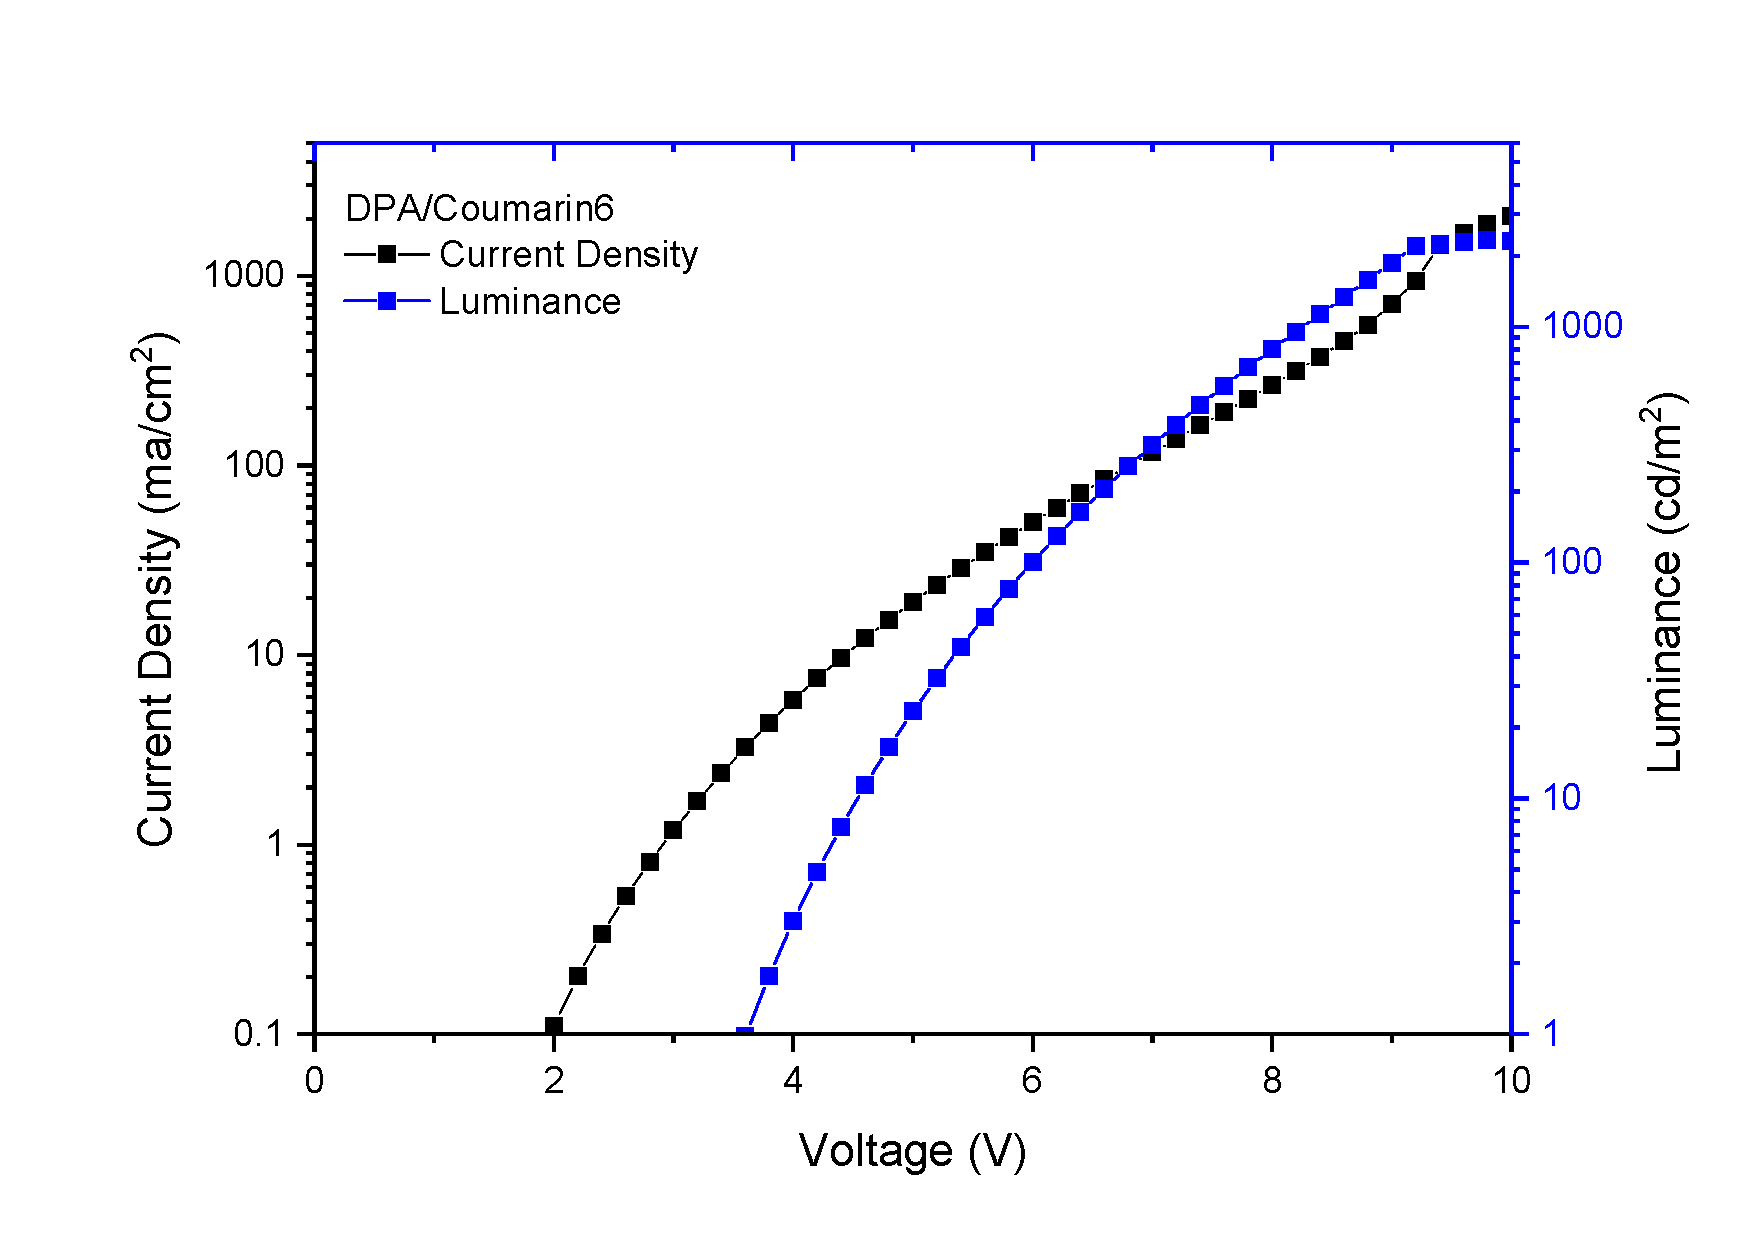
\includegraphics{./images/CoumarinJVL.pdf}

}

}

\subcaption{\label{fig-cjvl}}
\end{minipage}%
\newline
\begin{minipage}[t]{0.50\linewidth}

{\centering 

\raisebox{-\height}{

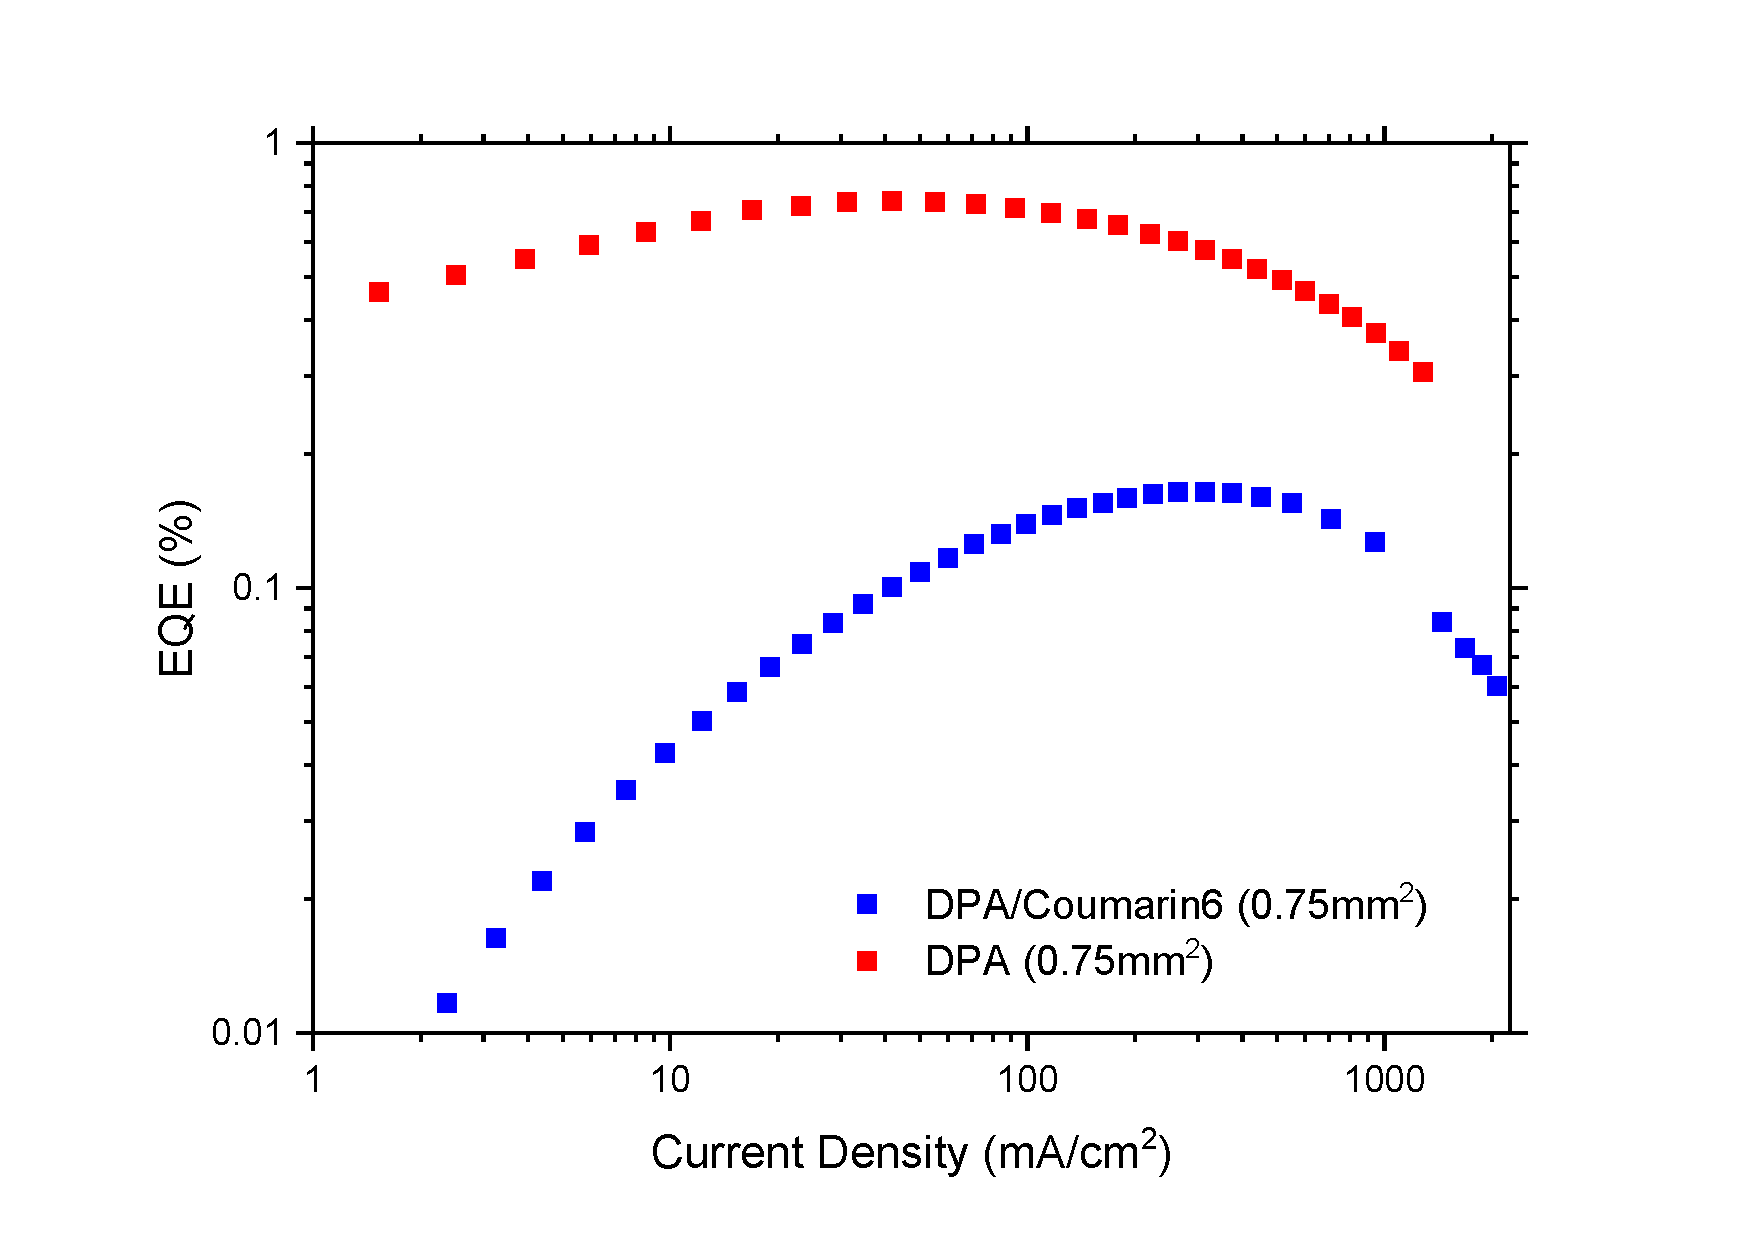
\includegraphics{./images/coumarinEQE.pdf}

}

}

\subcaption{\label{fig-ceqe}}
\end{minipage}%
%
\begin{minipage}[t]{0.50\linewidth}

{\centering 

\raisebox{-\height}{

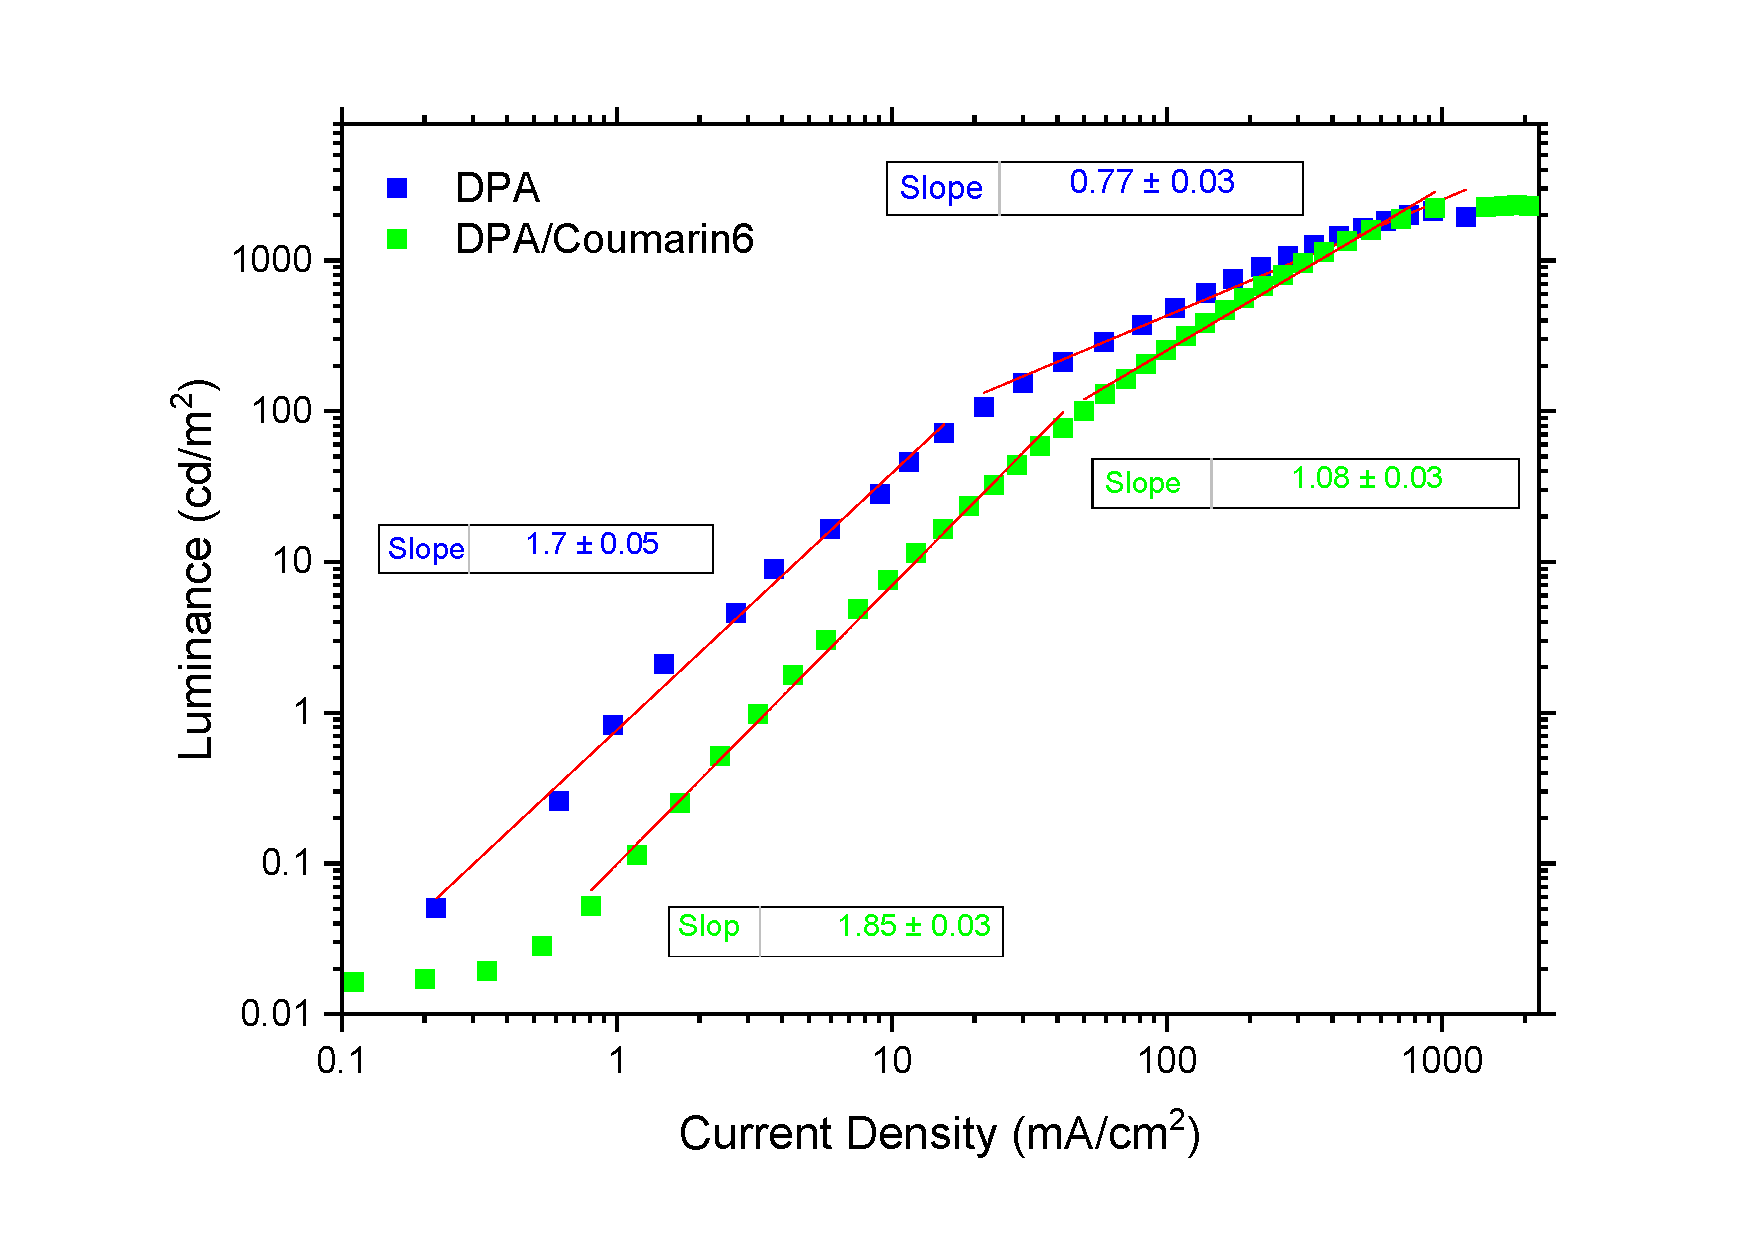
\includegraphics{./images/Coumarinslope.pdf}

}

}

\subcaption{\label{fig-cslope}}
\end{minipage}%

\caption{\label{fig-cstuff}Figure (a) Electroluminescence spectra of
neat film 2,6-DPA compared to it doped in {1wt\%} Coumarin6 (b) Current
density-luminance-voltage (J-V-L) graph of 2,6-DPA/Coumarin6 neat films
(b) EQE versus current density graph of doped films (d) Luminance versus
current density graph showing the two regimes of TTU-dominant and
STA-dominant}

\end{figure}

Four neat film devices were fabricated each having eight pixels (four
\(0.75mm^2\) and four \(0.3mm^2\)). Due to faulty contacts, thermal
evaporation alignment issues, and scratches or blemishes on the
substrate window some pixels become unable to be tested. Others can
degrade whilst a voltage is applied. In these doped-OLEDs, a majority
were unstable due to fabrication issues. A few pixels managed to
survive. A turn-on voltage of \(3.6\pm0.2\) V was achieved at the
defined \(1 cd/m^2\), with the maximum brightness approaching
\(2300\pm1000 cd/m^2\) at \(10\pm0.2\) V. The large uncertainty for
maximum brightness is too account for minimal pixel survival rate. The
J-V-L characteristics of the doped film and the EQE versus current
density graph can be found in Figure~\ref{fig-cjvl} and
Figure~\ref{fig-ceqe}. A roll up of EQE (peak \(0.16\pm0.10\)\%) until
\(~500\pm200 mA/cm^2\) demonstrates early triplet-triplet upconversion
gain (see Figure~\ref{fig-ceqe}). The peak EQE of this device, however,
do not exceed the theoretical maximum EQE of \(~2.25\%\). It also is
noticeably lower than 2,6-DPA neat film. This could be due to failure to
achieve \(1-2wt\%\) because of limitations with the thermal evaporator.
It could also be device structure that might not present good injection
of charges. The doped film exhibits similar luminance-current density
trends with its distinct two-regimes of slope \(>1\) and \(<1\) (see
Figure~\ref{fig-cslope}). The transition current density is roughly
\(900\pm100 mA/cm^2\). The slope is \(<2\) due to imperfect TTU and
losses, such as STA and other quenching. An observed slope shift from
\(>1\) to \(<1\) indicates definite gain of triplet to singlet excitons.

Pulse measurements (transient electroluminescence) will demonstrate the
population dynamics of the excitons even to high current densities. The
device area used was \(0.7mm^2\) to reduce geometrical capacitance that
minimises RC response distortion. For doped films, a long pulse width
(\(1.5\mu s\)) was used to extrapolate the affect STA had on fluorescent
materials at high current densities. Whilst DC measurements only reached
current densities of \(1 A/cm^2\), pulse measurements reach densities of
\(>2.5 A/cm^2\). At high current densities, doped and non-doped devices
show a sharp rise, characteristic of space charge limited current
conditions), with the initial rise lifetime of \(~80 ns\). This is
characteristic of TTU devices because of the recycling nature of the
triplet excitons generating additional singlets. At high current
densities (40 V) the steady state shows decrease over time, indicating
STA has dominated rate over the TTU generation rate (see
Figure~\ref{fig-cslope}). This decrease is more than the neat-film,
indicating that TTU either is not as present or STA is more dominant. At
lower current densities, STA is not prevalent so a steady state is
visible. STA dominates via FRET, a process that is determined by the
spectral overlap between \(S_1\) emission and \(T_1\rightarrow T_n\)
absorption bands.

\begin{figure}

\begin{minipage}[t]{0.50\linewidth}

{\centering 

\raisebox{-\height}{

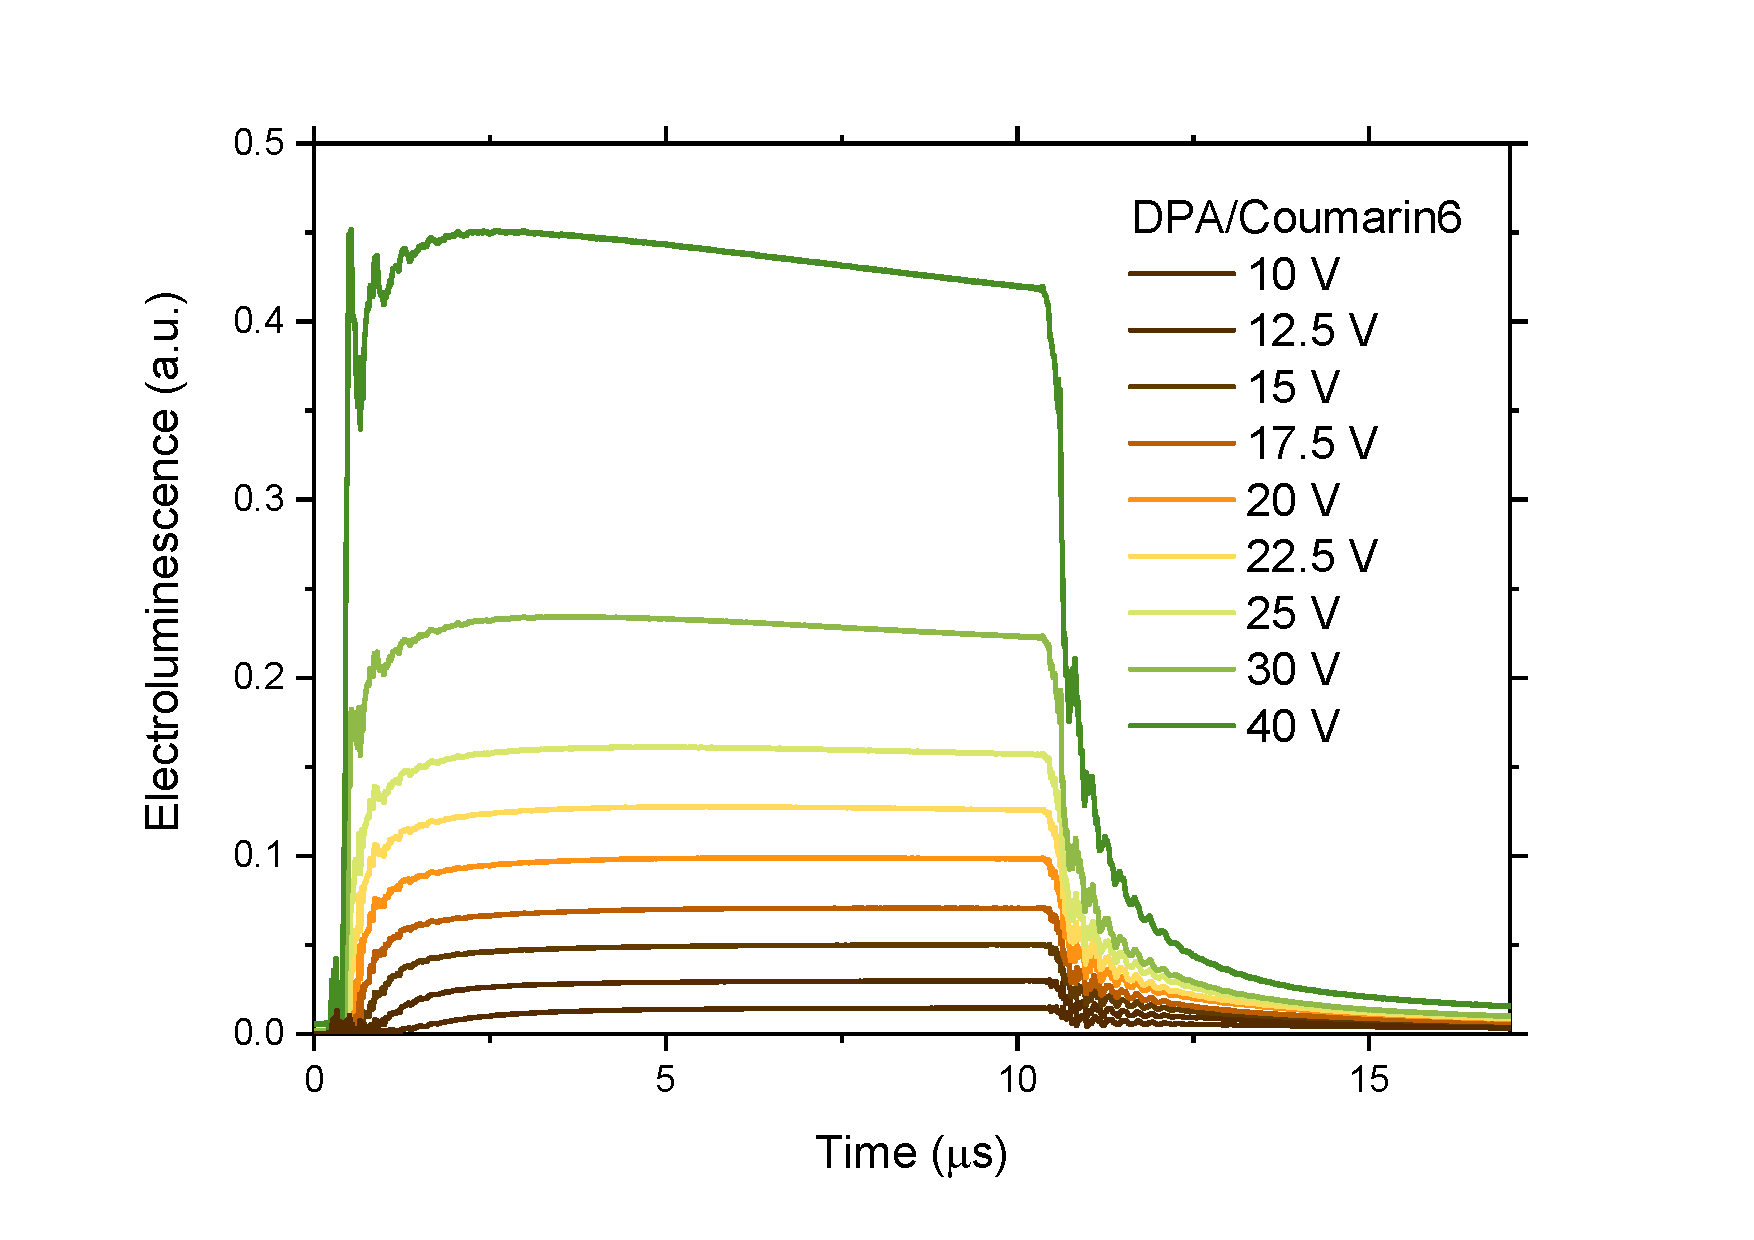
\includegraphics{./images/coumarinPULSE.pdf}

}

}

\subcaption{\label{fig-cpulsed}}
\end{minipage}%
%
\begin{minipage}[t]{0.50\linewidth}

{\centering 

\raisebox{-\height}{

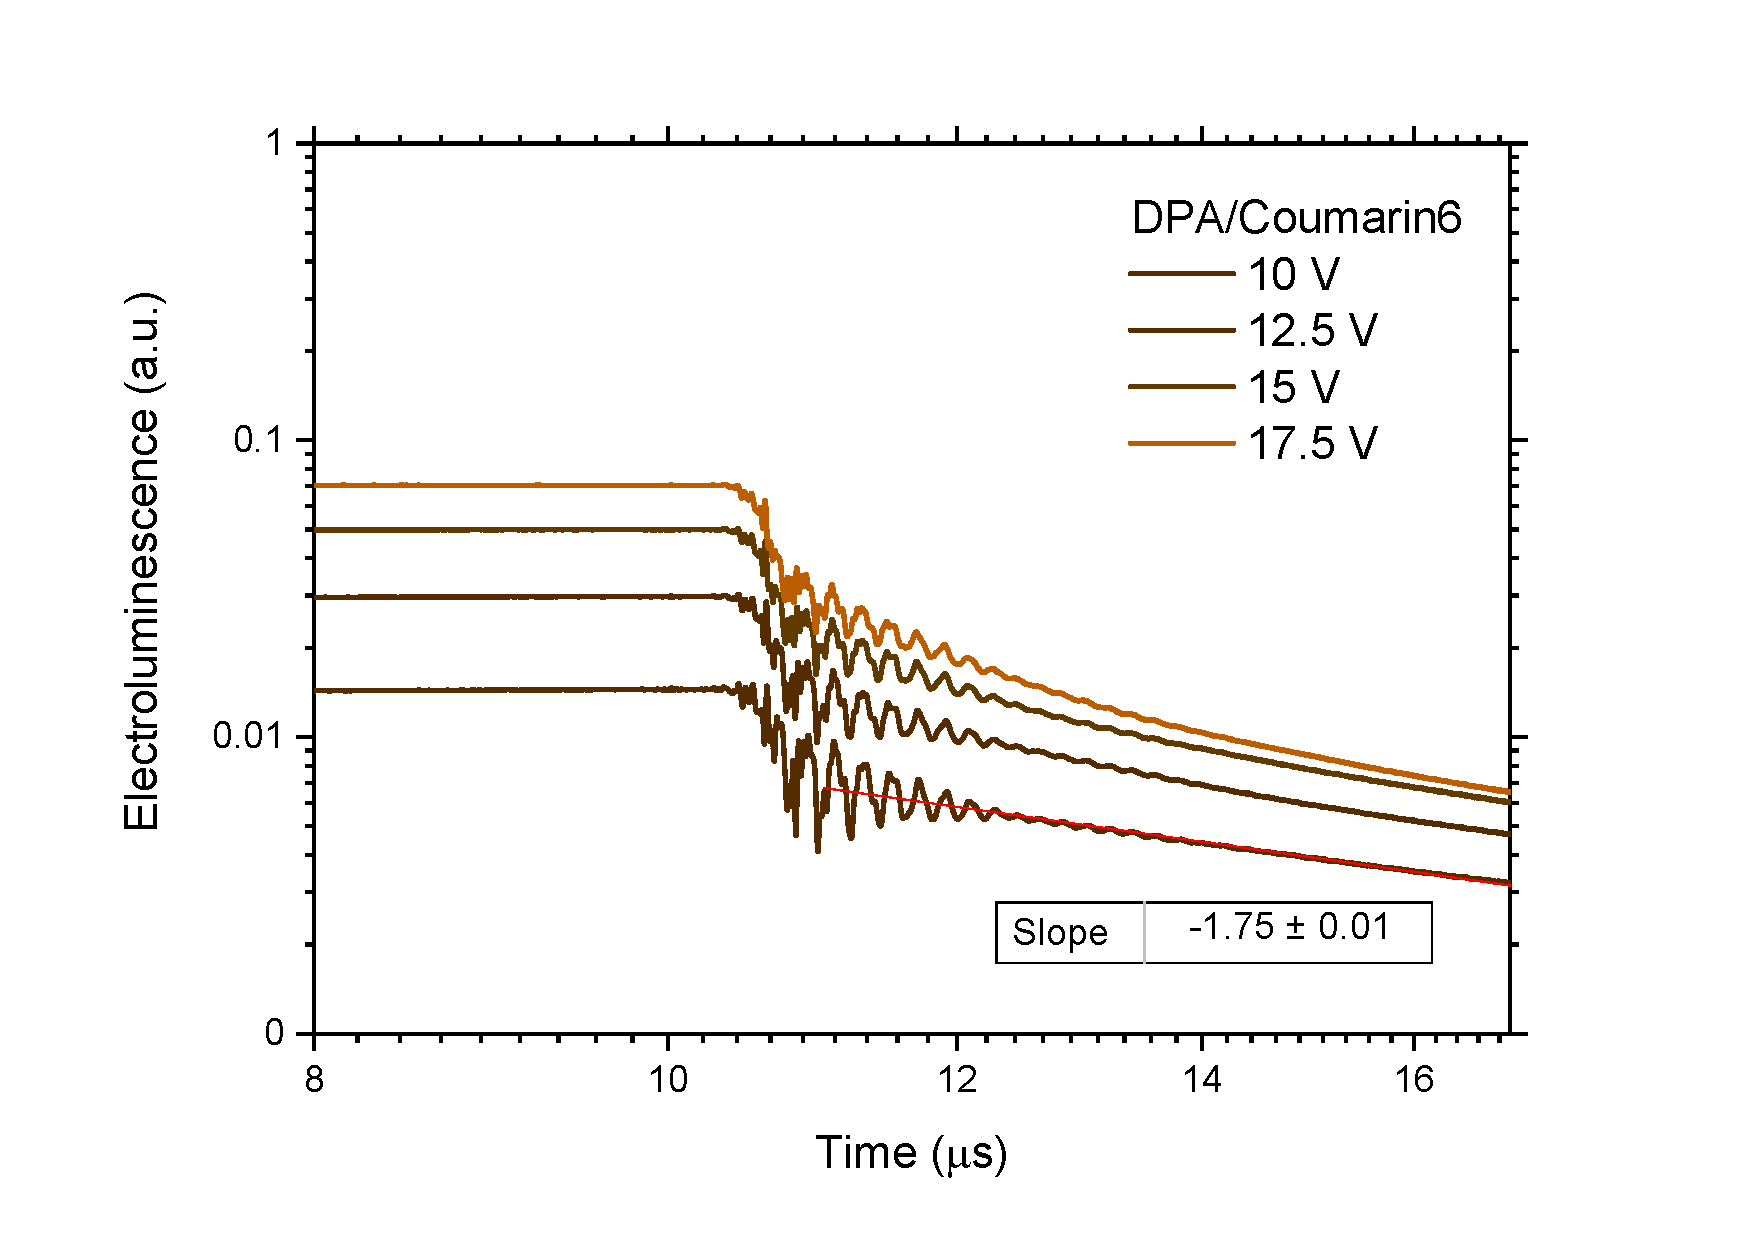
\includegraphics{./images/coumarinfitslope.pdf}

}

}

\subcaption{\label{fig-cfitslope}}
\end{minipage}%
\newline
\begin{minipage}[t]{\linewidth}

{\centering 

\raisebox{-\height}{

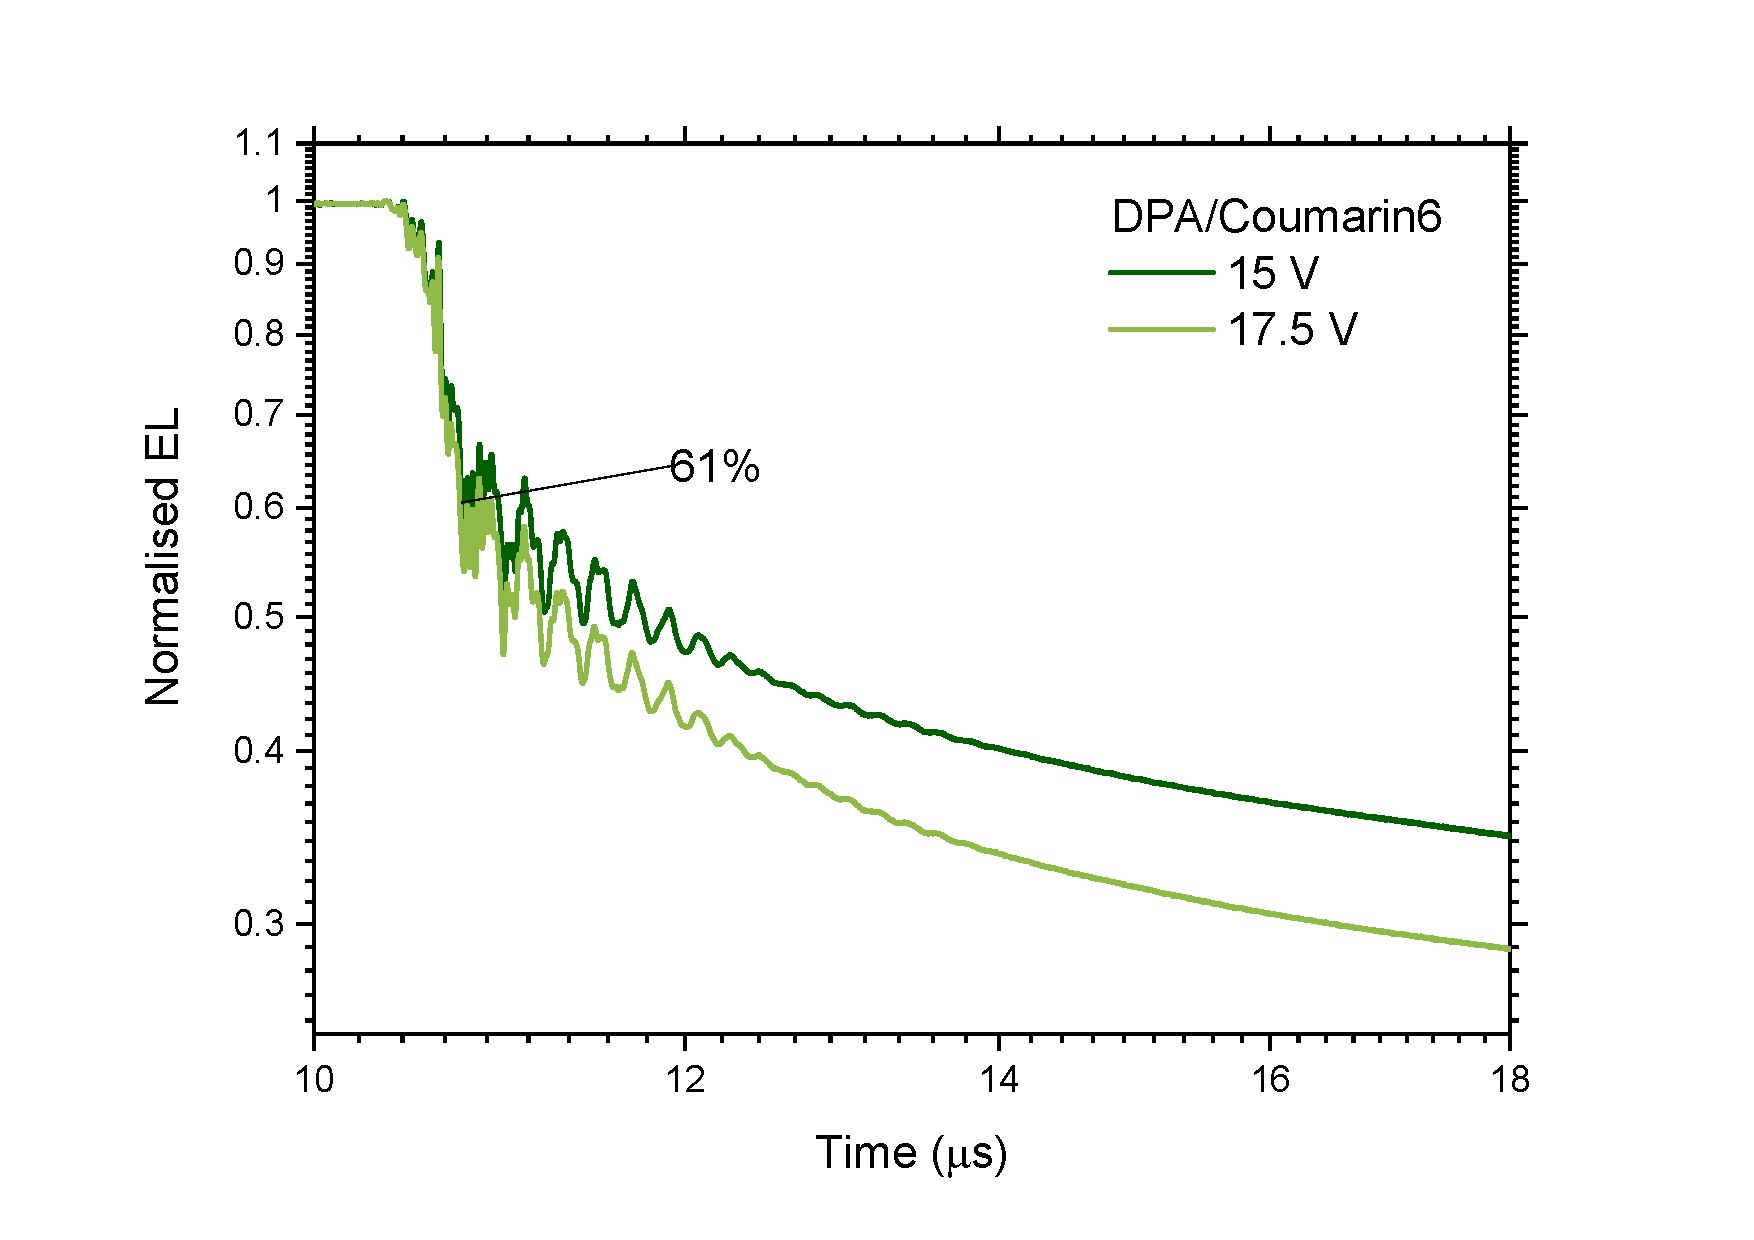
\includegraphics{./images/coumarinslopedata.pdf}

}

}

\subcaption{\label{fig-cslopedata}}
\end{minipage}%

\caption{\label{fig-cslope}Figure (a) Transient EL spectra of doped
2,6-DPA with Coumarin6 with a 1500 ns pulse width for many voltages. (b)
Log-log plot of the delayed fluorescence showing a slope of ~2 matching
TTU contribution (c) percentage fall from steady state to delayed
fluorescence}

\end{figure}

The turn off electroluminescence of pulse measurements also provide
useful information. For TTU devices, a prompt decay is expected after
voltage turn off due to the loss of direct singlet generation, followed
by a delayed fluorescence (DF) bimolecular decay function
\[EL_{DF} = \frac{1}{(a+bt)^2}\] where \(a\) and \(b\) are constants.
This characteristic slope of \(~2\) in a log-log plot can be observed in
these doped devices at low current density. The delayed component is
\(~61\%\) of the steady state (near TTU max) at \(15V\).

\hypertarget{discussion-1}{%
\subsection{Discussion}\label{discussion-1}}

2,6-DPA is an anthracene derivative with low PLQY and moderate charge
mobility in amorphous state. It can be doped with a higher PLQY material
to improve the overall efficiency. In neat film OLEDs, 2,6-DPA shows
distinctive TTU properties such as distinctive regimes as seen in the
mCBP OLEDs. This chapter uses the TTU property of 2,6-DPA to transfer
singlets to Coumarin6 via FRET (see Figure~\ref{fig-ttucoumarin}). A low
\(wt\%\) Coumarin6 was doped as to not separate the chromophores of
2,6-DPA, such that it would not extend the triplet states beyond the
short-range Dexter energy transfer process. This was successful as the
doped OLED showed trends of TTU. Despite the peak EQE not surpassing the
theoretical maximum of typical fluorescent emitters -- a feat that would
confirm extra exciton generation -- the evidence presented here is a
good start in showing this doped system exhibits TTU. To increase device
performance, optimisation of fabrication process and device structure
needs to be considered specific to an a 2,6-DPA/Coumarin6 host-guest
systems. Further optimisation of the thermal evaporation process would
also increase the pixel survivability and stability.

\bookmarksetup{startatroot}

\hypertarget{conclusion}{%
\chapter{Conclusion}\label{conclusion}}

Despite advertising this paper is on the path to electrically pumped
lasers, this thesis had its reticle focused on achieving triplet-triplet
annihilation upconversion in 2,6-DPA to dope it into typical fluorescent
lasing material, Coumarin6, to surpass its theoretical external quantum
efficiency maximum. While this thesis was not able to achieve an
increased performance on either device -- neat film 2,6-DPA or doped
2,6-DPA/Coumarin6 (1wt\%) -- the devices showed promise in exhibiting
TTU properties. It was confirmed in four different ways: displaying EQE
roll up at low current densities; demonstrating two distinct regimes in
a J-L log-log plot separated by a critical triplet density; transient
steady state electroluminescence progressively increasing over time at
low current densities; and transient electroluminescence delayed
fluorescence displaying the characteristic TTU curve. While these were
confirmed, to truly feel confident about TTU in these devices, the peak
EQE must surpass the theoretical maximum. This will be the next step.

The conclusions made from this work demonstrates the need to continue
down this path toward electrically pumped organic lasers. The future
work possible thanks to this thesis will be explained here.

\hypertarget{outlook}{%
\section{Outlook}\label{outlook}}

\hypertarget{optimization}{%
\subsection{Optimization}\label{optimization}}

The device in this thesis struggled to perform with high EQE. Particular
attention to optimisation of thermal evaporation needs to be considered,
to make the host-guest system of 2,6-DPA and Coumarin at \(1-2wt\%\)
comfortably achievable. Different device thickness could further
optimise injection and recombination of polarons. Further experiments to
optimize the results also need to be completed. Transient
electroluminescence of variant pulse widths to analyse the dynamics -- a
process that is a step towards simulating rate equations.

\hypertarget{simulate-rate-equations}{%
\subsection{Simulate rate equations}\label{simulate-rate-equations}}

Rate equations of STA and TTA need to be calculated from the singlet and
triplet population rate equations, such that the transient EL can be
analysed and understood. For example, this thesis only qualitatively
analyses the dominant STA and TTA process at low or high current
density. Simulation would provide rates that could be used to calculate
the necessary threshold current density for lasing. TTA becomes
important at high current density because of it is proportional to the
triplet population, \(n_T^2\), and STA is proportional to
\(n_{T1}n_{S1}\). Such a way to reduce STA, while keeping TTU high, is
to minimize the spectral overlap between the singlet and triplet
absorption spectrum.

\hypertarget{ase-measurements}{%
\subsection{ASE measurements}\label{ase-measurements}}

The first step in really testing lasing is via amplified spontaneous
emission (ASE). If the device experiences light amplification using a
TTU assisted emitter, it shows promise that lasing can be achieved. This
is because the ASE threshold can be converted into a singlet exciton
density threshold that can be used to calculated the current density
threshold. This can only be done with the rate equations of SSA, STA,
and TTA. However ASE measurements should be attacked only once higher
EQEs are reached.

\bookmarksetup{startatroot}

\hypertarget{references}{%
\chapter*{References}\label{references}}
\addcontentsline{toc}{chapter}{References}

\markboth{References}{References}

\hypertarget{refs}{}
\begin{CSLReferences}{1}{0}
\leavevmode\vadjust pre{\hypertarget{ref-RN47}{}}%
Adachi, Chihaya, Marc A. Baldo, Mark E. Thompson, and Stephen R.
Forrest. 2001. {``Nearly 100\% Internal Phosphorescence Efficiency in an
Organic Light-Emitting Device.''} Journal Article. \emph{Journal of
Applied Physics} 90 (10): 5048--51.
\url{https://doi.org/10.1063/1.1409582}.

\leavevmode\vadjust pre{\hypertarget{ref-RN9}{}}%
Adachi, Chihaya, and Atula S. D. Sandanayaka. 2020. {``The Leap from
Organic Light-Emitting Diodes to Organic Semiconductor Laser Diodes.''}
Journal Article. \emph{CCS Chemistry} 2 (4): 1203--16.
\url{https://doi.org/doi:10.31635/ccschem.020.202000327}.

\leavevmode\vadjust pre{\hypertarget{ref-RN49}{}}%
Adachi, Chihaya, Shizuo Tokito, Tetsuo Tsutsui, and Shogo Saito. 1988.
{``Electroluminescence in Organic Films with Three-Layer Structure.''}
Journal Article. \emph{Japanese Journal of Applied Physics} 27 (Part 2,
No. 2): L269--71. \url{https://doi.org/10.1143/jjap.27.l269}.

\leavevmode\vadjust pre{\hypertarget{ref-RN36}{}}%
Adachi, Chihaya, Tetsuo Tsutsui, and Shogo Saito. 1990. {``Blue
Light‐emitting Organic Electroluminescent Devices.''} Journal Article.
\emph{Applied Physics Letters} 56 (9): 799--801.
\url{https://doi.org/10.1063/1.103177}.

\leavevmode\vadjust pre{\hypertarget{ref-RN41}{}}%
Agrawal, Saurabh, Pratibha Dev, Niall J. English, K. Ravindranathan
Thampi, and J. M. D. MacElroy. 2011. {``First-Principles Study of the
Excited-State Properties of Coumarin-Derived Dyes in Dye-Sensitized
Solar Cells.''} Journal Article. \emph{Journal of Materials Chemistry}
21 (30): 11101--8. \url{https://doi.org/10.1039/C1JM10953G}.

\leavevmode\vadjust pre{\hypertarget{ref-RN145}{}}%
Atul, Shukla, Hasan Monirul, Banappanavar Gangadhar, Ahmad Viqar, Sobus
Jan, Moore Evan, Kabra Dinesh, Lo Shih-Chun, and Namdas Ebinazar. 2021.
Journal Article. \emph{Research Square}.
\url{https://doi.org/10.21203/rs.3.rs-74957/v1}.

\leavevmode\vadjust pre{\hypertarget{ref-RN50}{}}%
Aziz, Hany, Zoran D. Popovic, Nan-Xing Hu, Ah-Mee Hor, and Gu Xu. 1999.
{``Degradation Mechanism of Small Molecule-Based Organic Light-Emitting
Devices.''} Journal Article. \emph{Science} 283 (5409): 1900--1902.
\url{https://doi.org/doi:10.1126/science.283.5409.1900}.

\leavevmode\vadjust pre{\hypertarget{ref-RN20}{}}%
Baldo, M. A., R. J. Holmes, and S. R. Forrest. 2002. {``Prospects for
Electrically Pumped Organic Lasers.''} Journal Article. \emph{Physical
Review B} 66 (3): 035321.
\url{https://doi.org/10.1103/PhysRevB.66.035321}.

\leavevmode\vadjust pre{\hypertarget{ref-RN48}{}}%
Baldo, M. A., S. Lamansky, P. E. Burrows, M. E. Thompson, and S. R.
Forrest. 1999. {``Very High-Efficiency Green Organic Light-Emitting
Devices Based on Electrophosphorescence.''} Journal Article.
\emph{Applied Physics Letters} 75 (1): 4--6.
\url{https://doi.org/10.1063/1.124258}.

\leavevmode\vadjust pre{\hypertarget{ref-RN22}{}}%
Baldo, M. A., D. F. O'Brien, Y. You, A. Shoustikov, S. Sibley, M. E.
Thompson, and S. R. Forrest. 1998. {``Highly Efficient Phosphorescent
Emission from Organic Electroluminescent Devices.''} Journal Article.
\emph{Nature} 395 (6698): 151--54. \url{https://doi.org/10.1038/25954}.

\leavevmode\vadjust pre{\hypertarget{ref-RN6}{}}%
Burroughes, J. H., D. D. C. Bradley, A. R. Brown, R. N. Marks, K.
Mackay, R. H. Friend, P. L. Burns, and A. B. Holmes. 1990.
{``Light-Emitting Diodes Based on Conjugated Polymers.''} Journal
Article. \emph{Nature} 347 (6293): 539--41.
\url{https://doi.org/10.1038/347539a0}.

\leavevmode\vadjust pre{\hypertarget{ref-RN64}{}}%
Cai, Yuan-yuan, Xiao Chen, Ning Li, Chang-wei Li, and Yi-quan Wang.
2017. {``Electrically Pumped Photonic Crystal Laser Constructed with
Organic Semiconductors.''} Journal Article. \emph{Laser Physics} 27 (3):
035801. \url{https://doi.org/10.1088/1555-6611/aa5291}.

\leavevmode\vadjust pre{\hypertarget{ref-RN55}{}}%
Cester, A., D. Bari, J. Framarin, N. Wrachien, G. Meneghesso, S. Xia, V.
Adamovich, and J. J. Brown. 2010. {``Thermal and Electrical Stress
Effects of Electrical and Optical Characteristics of Alq3/NPD OLED.''}
Journal Article. \emph{Microelectronics Reliability} 50 (9): 1866--70.
https://doi.org/\url{https://doi.org/10.1016/j.microrel.2010.07.114}.

\leavevmode\vadjust pre{\hypertarget{ref-RN91}{}}%
Chakaroun, M., A. Coens, N. Fabre, F. Gourdon, J. Solard, A. Fischer, A.
Boudrioua, and C. C. Lee. 2011. {``Optimal Design of a Microcavity
Organic Laser Device Under Electrical Pumping.''} Journal Article.
\emph{Optics Express} 19 (2): 493--505.
\url{https://doi.org/10.1364/OE.19.000493}.

\leavevmode\vadjust pre{\hypertarget{ref-RN131}{}}%
Chen, Yi-Hsiang, Chih-Chun Lin, Min-Jie Huang, Kevin Hung, Yi-Ching Wu,
Wei-Chieh Lin, Ren-Wu Chen-Cheng, Hao-Wu Lin, and Chien-Hong Cheng.
2016. {``Superior Upconversion Fluorescence Dopants for Highly Efficient
Deep-Blue Electroluminescent Devices.''} Journal Article. \emph{Chemical
Science} 7 (7): 4044--51. \url{https://doi.org/10.1039/C6SC00100A}.

\leavevmode\vadjust pre{\hypertarget{ref-RN143}{}}%
Chen, Yongzhen, Xiaofang Wei, Zhiyi Li, Yanwei Liu, Jianjun Liu, Ruifang
Wang, Pengfei Wang, Yukiko Yamada-Takamura, and Ying Wang. 2017.
{``N-Doping-Induced Efficient Electron-Injection for High Efficiency
Inverted Organic Light-Emitting Diodes Based on Thermally Activated
Delayed Fluorescence Emitter.''} Journal Article. \emph{Journal of
Materials Chemistry C} 5 (33): 8400--8407.
\url{https://doi.org/10.1039/C7TC02406A}.

\leavevmode\vadjust pre{\hypertarget{ref-RN128}{}}%
Chou, P. Y., H. H. Chou, Y. H. Chen, T. H. Su, C. Y. Liao, H. W. Lin, W.
C. Lin, H. Y. Yen, I. C. Chen, and C. H. Cheng. 2014. {``Efficient
Delayed Fluorescence via Triplet--Triplet Annihilation for Deep-Blue
Electroluminescence.''} Journal Article. \emph{Chemical Communications}
50 (52): 6869--71. \url{https://doi.org/10.1039/C4CC01851F}.

\leavevmode\vadjust pre{\hypertarget{ref-RN45}{}}%
Coropceanu, Veaceslav, Jérôme Cornil, Demetrio A. da Silva Filho, Yoann
Olivier, Robert Silbey, and Jean-Luc Brédas. 2007. {``Charge Transport
in Organic Semiconductors.''} Journal Article. \emph{Chemical Reviews}
107 (4): 926--52. \url{https://doi.org/10.1021/cr050140x}.

\leavevmode\vadjust pre{\hypertarget{ref-RN2}{}}%
Dantus, M., R. M. Bowman, and A. H. Zewail. 1990. {``Femtosecond Laser
Observations of Molecular Vibration and Rotation.''} Journal Article.
\emph{Nature} 343 (6260): 737--39.
\url{https://doi.org/10.1038/343737a0}.

\leavevmode\vadjust pre{\hypertarget{ref-RN147}{}}%
Debye, P., and John O. Edwards. 1952. {``Long‐lifetime Phosphorescence
and the Diffusion Process.''} Journal Article. \emph{The Journal of
Chemical Physics} 20 (2): 236--39.
\url{https://doi.org/10.1063/1.1700385}.

\leavevmode\vadjust pre{\hypertarget{ref-RN85}{}}%
Dexter, D. L. 1953. {``A Theory of Sensitized Luminescence in Solids.''}
Journal Article. \emph{The Journal of Chemical Physics} 21 (5): 836--50.
\url{https://doi.org/10.1063/1.1699044}.

\leavevmode\vadjust pre{\hypertarget{ref-RN28}{}}%
Di, Dawei, Le Yang, Johannes M. Richter, Lorenzo Meraldi, Rashid M.
Altamimi, Ahmed Y. Alyamani, Dan Credgington, Kevin P. Musselman, Judith
L. MacManus-Driscoll, and Richard H. Friend. 2017. {``Efficient Triplet
Exciton Fusion in Molecularly Doped Polymer Light-Emitting Diodes.''}
Journal Article. \emph{Advanced Materials} 29 (13): 1605987.
https://doi.org/\url{https://doi.org/10.1002/adma.201605987}.

\leavevmode\vadjust pre{\hypertarget{ref-RN37}{}}%
Djurovich, Peter I., Elizabeth I. Mayo, Stephen R. Forrest, and Mark E.
Thompson. 2009. {``Measurement of the Lowest Unoccupied Molecular
Orbital Energies of Molecular Organic Semiconductors.''} Journal
Article. \emph{Organic Electronics} 10 (3): 515--20.
https://doi.org/\url{https://doi.org/10.1016/j.orgel.2008.12.011}.

\leavevmode\vadjust pre{\hypertarget{ref-RN58}{}}%
Duarte, F. J., L. S. Liao, and K. M. Vaeth. 2005. {``Coherence
Characteristics of Electrically Excited Tandem Organic Light-Emitting
Diodes.''} Journal Article. \emph{Optics Letters} 30 (22): 3072--74.
\url{https://doi.org/10.1364/OL.30.003072}.

\leavevmode\vadjust pre{\hypertarget{ref-RN3}{}}%
Duarte, Vaeth, F. J. 2018. {``Organic Lasers and Organic Photonics.''}
Electronic Book. IOP Publishing.
\url{https://doi.org/10.1088/978-0-7503-1572-2}.

\leavevmode\vadjust pre{\hypertarget{ref-RN122}{}}%
Dzebo, Damir, Karl Börjesson, Victor Gray, Kasper Moth-Poulsen, and Bo
Albinsson. 2016. {``Intramolecular Triplet--Triplet Annihilation
Upconversion in 9,10-Diphenylanthracene Oligomers and Dendrimers.''}
Journal Article. \emph{The Journal of Physical Chemistry C} 120 (41):
23397--406. \url{https://doi.org/10.1021/acs.jpcc.6b07920}.

\leavevmode\vadjust pre{\hypertarget{ref-RN57}{}}%
El-Nadi, Lotfia, Latifa Al-Houty, M. M. Omar, and M. Ragab. 1998.
{``Organic Thin Film Materials Producing Novel Blue Laser.''} Journal
Article. \emph{Chemical Physics Letters} 286 (1): 9--14.
https://doi.org/\url{https://doi.org/10.1016/S0009-2614(98)00066-9}.

\leavevmode\vadjust pre{\hypertarget{ref-RN113}{}}%
Engmann, Sebastian, Adam J. Barito, Emily G. Bittle, Noel C. Giebink,
Lee J. Richter, and David J. Gundlach. 2019. {``Reply to:
Triplet-Triplet Annihilation in Rubrene/C60 OLEDs with
Electroluminescence Turn-on Breaking the Thermodynamic Limit.''} Journal
Article. \emph{Nature Communications} 10 (1): 4684.
\url{https://doi.org/10.1038/s41467-019-12598-4}.

\leavevmode\vadjust pre{\hypertarget{ref-RN4}{}}%
Forget, Sébastien, and Sébastien Chénais. 2013. \emph{Organic
Solid-State Lasers}. Book. 1st ed. 2013. Berlin, Heidelberg: Springer
Berlin Heidelberg : Imprint: Springer.

\leavevmode\vadjust pre{\hypertarget{ref-RN130}{}}%
Fukagawa, Hirohiko, Takahisa Shimizu, Noriyuki Ohbe, Shizuo Tokito,
Katsumi Tokumaru, and Hideo Fujikake. 2012. {``Anthracene Derivatives as
Efficient Emitting Hosts for Blue Organic Light-Emitting Diodes
Utilizing Triplet--Triplet Annihilation.''} Journal Article.
\emph{Organic Electronics} 13 (7): 1197--1203.
https://doi.org/\url{https://doi.org/10.1016/j.orgel.2012.03.019}.

\leavevmode\vadjust pre{\hypertarget{ref-RN125}{}}%
Gao, Can, Shyamal K. K. Prasad, Bolong Zhang, Miroslav Dvořák, Murad J.
Y. Tayebjee, Dane R. McCamey, Timothy W. Schmidt, Trevor A. Smith, and
Wallace W. H. Wong. 2019. {``Intramolecular Versus Intermolecular
Triplet Fusion in Multichromophoric Photochemical Upconversion.''}
Journal Article. \emph{The Journal of Physical Chemistry C} 123 (33):
20181--87. \url{https://doi.org/10.1021/acs.jpcc.9b07098}.

\leavevmode\vadjust pre{\hypertarget{ref-RN21}{}}%
Gao, Can, Wallace W. H. Wong, Zhengsheng Qin, Shih-Chun Lo, Ebinazar B.
Namdas, Huanli Dong, and Wenping Hu. 2021. {``Application of
Triplet--Triplet Annihilation Upconversion in Organic Optoelectronic
Devices: Advances and Perspectives.''} Journal Article. \emph{Advanced
Materials} n/a (n/a): 2100704.
https://doi.org/\url{https://doi.org/10.1002/adma.202100704}.

\leavevmode\vadjust pre{\hypertarget{ref-RN81}{}}%
Gärtner, Christian. 2009. \emph{Organic Laser Diodes: Modelling and
Simulation}. Book.

\leavevmode\vadjust pre{\hypertarget{ref-RN109}{}}%
Giebink, N. C., and S. R. Forrest. 2008. {``Quantum Efficiency Roll-Off
at High Brightness in Fluorescent and Phosphorescent Organic Light
Emitting Diodes.''} Journal Article. \emph{Physical Review B} 77 (23):
235215. \url{https://doi.org/10.1103/PhysRevB.77.235215}.

\leavevmode\vadjust pre{\hypertarget{ref-RN69}{}}%
---------. 2009. {``Temporal Response of Optically Pumped Organic
Semiconductor Lasers and Its Implication for Reaching Threshold Under
Electrical Excitation.''} Journal Article. \emph{Physical Review B} 79
(7): 073302. \url{https://doi.org/10.1103/PhysRevB.79.073302}.

\leavevmode\vadjust pre{\hypertarget{ref-RN68}{}}%
Giebink, N. C., Y. Sun, and S. R. Forrest. 2006. {``Transient Analysis
of Triplet Exciton Dynamics in Amorphous Organic Semiconductor Thin
Films.''} Journal Article. \emph{Organic Electronics} 7 (5): 375--86.
https://doi.org/\url{https://doi.org/10.1016/j.orgel.2006.04.007}.

\leavevmode\vadjust pre{\hypertarget{ref-RN10}{}}%
Goossens, Mark, Arvydas Ruseckas, Graham A. Turnbull, and Ifor D. W.
Samuel. 2004. {``Subpicosecond Pulses from a Gain-Switched Polymer
Distributed Feedback Laser.''} Journal Article. \emph{Applied Physics
Letters} 85 (1): 31--33. \url{https://doi.org/10.1063/1.1767952}.

\leavevmode\vadjust pre{\hypertarget{ref-RN102}{}}%
Görrn, P., T. Rabe, T. Riedl, and W. Kowalsky. 2007. {``Loss Reduction
in Fully Contacted Organic Laser Waveguides Using TE2 Modes.''} Journal
Article. \emph{Applied Physics Letters} 91 (4): 041113.
\url{https://doi.org/10.1063/1.2757598}.

\leavevmode\vadjust pre{\hypertarget{ref-RN82}{}}%
Heeger, Alan J. 2001. {``Nobel Lecture: Semiconducting and Metallic
Polymers: The Fourth Generation of Polymeric Materials*.''} Journal
Article. \emph{Reviews of Modern Physics} 73: 681--700.

\leavevmode\vadjust pre{\hypertarget{ref-RN8}{}}%
Hide, Fumitomo, Maria A. Diaz-Garcia, Benjamin J. Schwartz, Mats R.
Andersson, and et al. 1996. {``Semiconducting Polymers: A New Class of
Solid-State Laser Materials.''} Journal Article. \emph{Science} 273
(5283): 1833.
\href{https://proquest.com/scholarly-journals/semiconducting-polymers-new-class-solid-state}{proquest.com/scholarly-journals/semiconducting-polymers-new-class-solid-state}.

\leavevmode\vadjust pre{\hypertarget{ref-RN97}{}}%
Hill, Martin T., and Malte C. Gather. 2014. {``Advances in Small
Lasers.''} Journal Article. \emph{Nature Photonics} 8 (12): 908--18.
\url{https://doi.org/10.1038/nphoton.2014.239}.

\leavevmode\vadjust pre{\hypertarget{ref-RN108}{}}%
Ieuji, Ryota, Kenichi Goushi, and Chihaya Adachi. 2019.
{``Triplet--Triplet Upconversion Enhanced by Spin--Orbit Coupling in
Organic Light-Emitting Diodes.''} Journal Article. \emph{Nature
Communications} 10 (1): 5283.
\url{https://doi.org/10.1038/s41467-019-13044-1}.

\leavevmode\vadjust pre{\hypertarget{ref-RN144}{}}%
Ihn, Soo-Ghang, Namheon Lee, Soon Ok Jeon, Myungsun Sim, Hosuk Kang,
Yongsik Jung, Dal Ho Huh, et al. 2017. {``An Alternative Host Material
for Long-Lifespan Blue Organic Light-Emitting Diodes Using Thermally
Activated Delayed Fluorescence.''} Journal Article. \emph{Advanced
Science} 4 (8): 1600502.
https://doi.org/\url{https://doi.org/10.1002/advs.201600502}.

\leavevmode\vadjust pre{\hypertarget{ref-RN26}{}}%
Im, Yirang, Seong Yong Byun, Ji Han Kim, Dong Ryun Lee, Chan Seok Oh,
Kyoung Soo Yook, and Jun Yeob Lee. 2017. {``Recent Progress in
High-Efficiency Blue-Light-Emitting Materials for Organic Light-Emitting
Diodes.''} Journal Article. \emph{Advanced Functional Materials} 27
(13): 1603007.
https://doi.org/\url{https://doi.org/10.1002/adfm.201603007}.

\leavevmode\vadjust pre{\hypertarget{ref-RN65}{}}%
Jacko, A. C., Ross H. McKenzie, and B. J. Powell. 2010. {``Models of
Organometallic Complexes for Optoelectronic Applications.''} Journal
Article. \emph{Journal of Materials Chemistry} 20 (46): 10301--7.
\url{https://doi.org/10.1039/C0JM01786H}.

\leavevmode\vadjust pre{\hypertarget{ref-RN77}{}}%
Jenekhe, Samson A. 1986. {``A Class of Narrow-Band-Gap Semiconducting
Polymers.''} Journal Article. \emph{Nature} 322 (6077): 345--47.
\url{https://doi.org/10.1038/322345a0}.

\leavevmode\vadjust pre{\hypertarget{ref-RN54}{}}%
Jiang, Xue-Yin, Zhi-Lin Zhang, Jin Cao, M. A. Khan, Haq Khizar ul, and
Wen-Qing Zhu. 2007. {``White OLED with High Stability and Low Driving
Voltage Based on a Novel Buffer Layer MoOx.''} Journal Article.
\emph{Journal of Physics D: Applied Physics} 40 (18): 5553--57.
\url{https://doi.org/10.1088/0022-3727/40/18/007}.

\leavevmode\vadjust pre{\hypertarget{ref-RN148}{}}%
Kabe, Ryota, and Chihaya Adachi. 2017. {``Organic Long Persistent
Luminescence.''} Journal Article. \emph{Nature} 550 (7676): 384--87.
\url{https://doi.org/10.1038/nature24010}.

\leavevmode\vadjust pre{\hypertarget{ref-RN133}{}}%
Kabra, Dinesh, Li Ping Lu, Myoung Hoon Song, Henry J. Snaith, and
Richard H. Friend. 2010. {``Efficient Single-Layer Polymer
Light-Emitting Diodes.''} Journal Article. \emph{Advanced Materials} 22
(29): 3194--98.
https://doi.org/\url{https://doi.org/10.1002/adma.201000317}.

\leavevmode\vadjust pre{\hypertarget{ref-RN95}{}}%
Kallinger, Christian, Martin Hilmer, Andreas Haugeneder, Martin Perner,
Wolfgang Spirkl, Uli Lemmer, Jochen Feldmann, et al. 1998. {``A Flexible
Conjugated Polymer Laser.''} Journal Article. \emph{Adv. Mater} 10 (12):
920--23.
https://doi.org/\href{https://doi.org/10.1002/(SICI)1521-4095(199808)10:12\%3C920::AID-ADMA920\%3E3.0.CO\%0A2-7}{10.1002/(SICI)1521-4095(199808)10:12\textless920::AID-ADMA920\textgreater3.0.CO
2-7}.

\leavevmode\vadjust pre{\hypertarget{ref-RN11}{}}%
Karl, Markus, James M. E. Glackin, Marcel Schubert, Nils M. Kronenberg,
Graham A. Turnbull, Ifor D. W. Samuel, and Malte C. Gather. 2018.
{``Flexible and Ultra-Lightweight Polymer Membrane Lasers.''} Journal
Article. \emph{Nature Communications} 9 (1): 1525.
\url{https://doi.org/10.1038/s41467-018-03874-w}.

\leavevmode\vadjust pre{\hypertarget{ref-RN123}{}}%
Keivanidis, P. E., S. Baluschev, G. Lieser, and G. Wegner. 2009.
{``Inherent Photon Energy Recycling Effects in the up-Converted Delayed
Luminescence Dynamics of Poly(fluorene)--PtIIoctaethyl Porphyrin
Blends.''} Journal Article. \emph{ChemPhysChem} 10 (13): 2316--26.
https://doi.org/\url{https://doi.org/10.1002/cphc.200900290}.

\leavevmode\vadjust pre{\hypertarget{ref-RN70}{}}%
Kéna-Cohen, Stéphane, Aeneas Wiener, Yonatan Sivan, Paul N. Stavrinou,
Donal D. C. Bradley, Andrew Horsfield, and Stefan A. Maier. 2011.
{``Plasmonic Sinks for the Selective Removal of Long-Lived States.''}
Journal Article. \emph{ACS Nano} 5 (12): 9958--65.
\url{https://doi.org/10.1021/nn203754v}.

\leavevmode\vadjust pre{\hypertarget{ref-RN126}{}}%
Kido, Junji, and Yasuhiro Iizumi. 1998. {``Fabrication of Highly
Efficient Organic Electroluminescent Devices.''} Journal Article.
\emph{Applied Physics Letters} 73 (19): 2721--23.
\url{https://doi.org/10.1063/1.122570}.

\leavevmode\vadjust pre{\hypertarget{ref-RN149}{}}%
Kim, Jong Uk, In Seob Park, Chin-Yiu Chan, Masaki Tanaka, Youichi
Tsuchiya, Hajime Nakanotani, and Chihaya Adachi. 2020.
{``Nanosecond-Time-Scale Delayed Fluorescence Molecule for Deep-Blue
OLEDs with Small Efficiency Rolloff.''} Journal Article. \emph{Nature
Communications} 11 (1): 1765.
\url{https://doi.org/10.1038/s41467-020-15558-5}.

\leavevmode\vadjust pre{\hypertarget{ref-RN134}{}}%
Kim, Y. H., D. C. Shin, S.-H. Kim, C.-H. Ko, H.-S. Yu, Y.-S. Chae, and
S. K. Kwon. 2001. {``Novel Blue Emitting Material with High Color
Purity.''} Journal Article. \emph{Advanced Materials} 13 (22): 1690--93.
https://doi.org/\url{https://doi.org/10.1002/1521-4095(200111)13:22\%3C1690::AID-ADMA1690\%3E3.0.CO;2-K}.

\leavevmode\vadjust pre{\hypertarget{ref-RN106}{}}%
Köhler, A., and H. Bässler. 2009. {``Triplet States in Organic
Semiconductors.''} Journal Article. \emph{Materials Science and
Engineering: R: Reports} 66 (4): 71--109.
https://doi.org/\url{https://doi.org/10.1016/j.mser.2009.09.001}.

\leavevmode\vadjust pre{\hypertarget{ref-RN119}{}}%
Kondakov, Denis Y. 2015. {``Triplet--Triplet Annihilation in Highly
Efficient Fluorescent Organic Light-Emitting Diodes: Current State and
Future Outlook.''} Journal Article. \emph{Philosophical Transactions of
the Royal Society A: Mathematical, Physical and Engineering Sciences}
373 (2044): 20140321.

\leavevmode\vadjust pre{\hypertarget{ref-RN114}{}}%
Kondakov, Denis Y. 2009. {``Role of Triplet-Triplet Annihilation in
Highly Efficient Fluorescent Devices.''} Journal Article. \emph{Journal
of the Society for Information Display} 17 (2): 137--44.
https://doi.org/\url{https://doi.org/10.1889/JSID17.2.137}.

\leavevmode\vadjust pre{\hypertarget{ref-RN62}{}}%
Kozlov, V. G., V. Bulović, P. E. Burrows, and S. R. Forrest. 1997.
{``Laser Action in Organic Semiconductor Waveguide and
Double-Heterostructure Devices.''} Journal Article. \emph{Nature} 389:
362. \url{https://doi.org/10.1038/38693}.

\leavevmode\vadjust pre{\hypertarget{ref-RN63}{}}%
Kozlov, V. G., G. Parthasarathy, P. E. Burrows, V. B. Khalfin, J. Wang,
S. Y. Chou, and S. R. Forrest. 2000. {``Structures for Organic Diode
Lasers and Optical Properties of Organic Semiconductors Under Intense
Optical and Electrical Excitations.''} Journal Article. \emph{IEEE
Journal of Quantum Electronics} 36 (1): 18--26.
\url{https://doi.org/10.1109/3.817634}.

\leavevmode\vadjust pre{\hypertarget{ref-RN127}{}}%
Kuma, Hitoshi, and Chishio Hosokawa. 2014. {``Blue Fluorescent OLED
Materials and Their Application for High-Performance Devices.''} Journal
Article. \emph{Science and Technology of Advanced Materials} 15 (3):
034201. \url{https://doi.org/10.1088/1468-6996/15/3/034201}.

\leavevmode\vadjust pre{\hypertarget{ref-RN79}{}}%
Lakowicz, Joseph R. 2006. \emph{Principles of Fluorescence
Spectroscopy}. Book. 3rd ed. New York New York, NY: Springer Springer US
: Imprint: Springer.

\leavevmode\vadjust pre{\hypertarget{ref-RN100}{}}%
Lattante, S., F. Romano, A. P. Caricato, M. Martino, and M. Anni. 2006.
{``Low Electrode Induced Optical Losses in Organic Active Single Layer
Polyfluorene Waveguides with Two Indium Tin Oxide Electrodes Deposited
by Pulsed Laser Deposition.''} Journal Article. \emph{Applied Physics
Letters} 89 (3): 031108. \url{https://doi.org/10.1063/1.2222253}.

\leavevmode\vadjust pre{\hypertarget{ref-RN33}{}}%
Lawrence, Justin R., Graham A. Turnbull, Ifor D. W. Samuel, Gary J.
Richards, and Paul L. Burn. 2004. {``Optical Amplification in a
First-Generation Dendritic Organic Semiconductor.''} Journal Article.
\emph{Optics Letters} 29 (8): 869--71.
\url{https://doi.org/10.1364/OL.29.000869}.

\leavevmode\vadjust pre{\hypertarget{ref-RN90}{}}%
Lee, Chang-Lyoul, Xudong Yang, and Neil C. Greenham. 2007.
{``Determination of the Triplet Excited-State Absorption Cross Section
in a Polyfluorene by Energy Transfer from a Phosphorescent Metal
Complex.''} Journal Article. \emph{Physical Review B} 76 (24): 245201.
\url{https://doi.org/10.1103/PhysRevB.76.245201}.

\leavevmode\vadjust pre{\hypertarget{ref-RN140}{}}%
Lee, Sang-Bong, Takeshi Yasuda, Moon-Jae Yang, Katsuhiko Fujita, and
Tetsuo Tsutsui. 2003. {``CHARGE CARRIER MOBILITY IN VACUUM-SUBLIMED DYE
FILMS FOR LIGHT-EMITTING DIODES STUDIED BY THE TIME-OF-FLIGHT
TECHNIQUE.''} Journal Article. \emph{Molecular Crystals and Liquid
Crystals} 405 (1): 67--73.
\url{https://doi.org/10.1080/15421400390264162}.

\leavevmode\vadjust pre{\hypertarget{ref-RN104}{}}%
Lehnhardt, Marcus, Thomas Riedl, Torsten Rabe, and Wolfgang Kowalsky.
2011. {``Room Temperature Lifetime of Triplet Excitons in Fluorescent
Host/Guest Systems.''} Journal Article. \emph{Organic Electronics} 12:
486--91.

\leavevmode\vadjust pre{\hypertarget{ref-RN72}{}}%
Lehnhardt, M., T. Riedl, T. Weimann, and W. Kowalsky. 2010. {``Impact of
Triplet Absorption and Triplet-Singlet Annihilation on the Dynamics of
Optically Pumped Organic Solid-State Lasers.''} Journal Article.
\emph{Physical Review B} 81 (16): 165206.
\url{https://doi.org/10.1103/PhysRevB.81.165206}.

\leavevmode\vadjust pre{\hypertarget{ref-RN94}{}}%
Lemmer, Uli, Andreas Haugeneder, Christian Kallinger, and Jochen
Feldmann. 1999. {``Lasing in Conjugated Polymers.''} Book Section. In
\emph{Semiconducting Polymers}, 309--31.
https://doi.org/\url{https://doi.org/10.1002/3527602186.ch10}.

\leavevmode\vadjust pre{\hypertarget{ref-RN16}{}}%
Lenstra, Daan, Alexis P. A. Fischer, Amani Ouirimi, Alex C. Chime,
Nixson Loganathan, and Mahmoud Chakaroun. 2021. {``Organic Diode Laser
Dynamics: Rate-Equation Model, Reabsorption, Validation and Threshold
Predictions.''} Journal Article. \emph{Photonics} 8 (7).
\url{https://doi.org/10.3390/photonics8070279}.

\leavevmode\vadjust pre{\hypertarget{ref-RN43}{}}%
Li, Ling, and Hans Kosina. 2010. {``Charge Transport in Organic
Semiconductor Devices.''} Book Section. In \emph{Organic Electronics},
edited by Tibor Grasser, Gregor Meller, and Ling Li, 301--23. Berlin,
Heidelberg: Springer Berlin Heidelberg.
\url{https://doi.org/10.1007/12_2009_14}.

\leavevmode\vadjust pre{\hypertarget{ref-RN19}{}}%
Li, Yun, Randy P. Sabatini, Shyamal K. K. Prasad, Evan T. Hockings,
Timothy W. Schmidt, and Girish Lakhwani. 2021. {``Improved Optical
Confinement in Ambipolar Field-Effect Transistors Toward Electrical
Injection Organic Lasers.''} Journal Article. \emph{Applied Physics
Letters} 119 (16): 163303. \url{https://doi.org/10.1063/5.0063336}.

\leavevmode\vadjust pre{\hypertarget{ref-RN129}{}}%
Lim, Hyoungcheol, Hyung Jin Cheon, Gyeong Seok Lee, Mikyung Kim, Yun-Hi
Kim, and Jang-Joo Kim. 2019. {``Enhanced Triplet--Triplet Annihilation
of Blue Fluorescent Organic Light-Emitting Diodes by Generating Excitons
in Trapped Charge-Free Regions.''} Journal Article. \emph{ACS Applied
Materials \& Interfaces} 11 (51): 48121--27.
\url{https://doi.org/10.1021/acsami.9b15303}.

\leavevmode\vadjust pre{\hypertarget{ref-RN59}{}}%
Lin, Jie, Yongsheng Hu, Ying Lv, Xiaoyang Guo, and Xingyuan Liu. 2017.
{``Light Gain Amplification in Microcavity Organic Semiconductor Laser
Diodes Under Electrical Pumping.''} Journal Article. \emph{Science
Bulletin} 62 (24): 1637--38.
https://doi.org/\url{https://doi.org/10.1016/j.scib.2017.12.010}.

\leavevmode\vadjust pre{\hypertarget{ref-RN52}{}}%
Lin, Karen Ke, Soo Jin Chua, Wei-Wang, and Shuang Fang Lim. 2001.
{``Influence of Electrical Stress Voltage on Cathode Degradation of
Organic Light-Emitting Devices.''} Journal Article. \emph{Journal of
Applied Physics} 90 (2): 976--79.
\url{https://doi.org/10.1063/1.1376669}.

\leavevmode\vadjust pre{\hypertarget{ref-RN80}{}}%
List, E. J. W., U. Scherf, K. Müllen, W. Graupner, C. H. Kim, and J.
Shinar. 2002. {``Direct Evidence for Singlet-Triplet Exciton
Annihilation in \(\pi\)-Conjugated Polymers.''} Journal Article.
\emph{Physical Review B} 66 (23): 235203.
\url{https://doi.org/10.1103/PhysRevB.66.235203}.

\leavevmode\vadjust pre{\hypertarget{ref-RN138}{}}%
Liu, Hui, Liangliang Kang, Jinyu Li, Futong Liu, Xin He, Shenghong Ren,
Xiangyang Tang, Changli Lv, and Ping Lu. 2019. {``Highly Efficient
Deep-Blue Organic Light-Emitting Diodes Based on
Pyreno{[}4,5-d{]}imidazole-Anthracene Structural Isomers.''} Journal
Article. \emph{Journal of Materials Chemistry C} 7 (33): 10273--80.
\url{https://doi.org/10.1039/C9TC02990G}.

\leavevmode\vadjust pre{\hypertarget{ref-RN141}{}}%
Liu, Jie, Huanli Dong, Zongrui Wang, Deyang Ji, Changli Cheng, Hua Geng,
Hantang Zhang, et al. 2015. {``Thin Film Field-Effect Transistors of
2,6-Diphenyl Anthracene (DPA).''} Journal Article. \emph{Chemical
Communications} 51 (59): 11777--79.
\url{https://doi.org/10.1039/C4CC10348C}.

\leavevmode\vadjust pre{\hypertarget{ref-RN39}{}}%
Liu, Jie, Hantang Zhang, Huanli Dong, Lingqiang Meng, Longfeng Jiang,
Lang Jiang, Ying Wang, et al. 2015. {``High Mobility Emissive Organic
Semiconductor.''} Journal Article. \emph{Nature Communications} 6 (1):
10032. \url{https://doi.org/10.1038/ncomms10032}.

\leavevmode\vadjust pre{\hypertarget{ref-RN51}{}}%
Liu, Tswen-Hsin, Chung-Yeh Iou, and Chin H. Chen. 2003. {``Doped Red
Organic Electroluminescent Devices Based on a Cohost Emitter System.''}
Journal Article. \emph{Applied Physics Letters} 83 (25): 5241--43.
\url{https://doi.org/10.1063/1.1635986}.

\leavevmode\vadjust pre{\hypertarget{ref-RN139}{}}%
Liu, Wei, Shian Ying, Runda Guo, Xianfeng Qiao, Panpan Leng, Qing Zhang,
Yaxiong Wang, Dongge Ma, and Lei Wang. 2019. {``Nondoped Blue
Fluorescent Organic Light-Emitting Diodes Based on
Benzonitrile-Anthracene Derivative with 10.06 External Quantum
Efficiency and Low Efficiency Roll-Off.''} Journal Article.
\emph{Journal of Materials Chemistry C} 7 (4): 1014--21.
\url{https://doi.org/10.1039/C8TC05707A}.

\leavevmode\vadjust pre{\hypertarget{ref-RN60}{}}%
Liu, Xingyuan, Huibin Li, Chunyan Song, Yaqin Liao, and Miaomiao Tian.
2009. {``Microcavity Organic Laser Device Under Electrical Pumping.''}
Journal Article. \emph{Optics Letters} 34 (4): 503--5.
\url{https://doi.org/10.1364/OL.34.000503}.

\leavevmode\vadjust pre{\hypertarget{ref-RN116}{}}%
Luo, Yan-Ju, Zhi-Yun Lu, and Yan Huang. 2016. {``Triplet Fusion Delayed
Fluorescence Materials for OLEDs.''} Journal Article. \emph{Chinese
Chemical Letters} 27 (8): 1223--30.
https://doi.org/\url{https://doi.org/10.1016/j.cclet.2016.06.002}.

\leavevmode\vadjust pre{\hypertarget{ref-RN84}{}}%
Lupton, John M., Martin Reufer, Manfred J. Walter, Pavlos G. Lagoudakis,
Anne Beate Hummel, Johanna S. Kolb, Hartmut G. Roskos, and Ullrich
Scherf. 2005. {``Spin-Conserving Carrier Recombination in Conjugated
Polymers.''} Journal Article. \emph{Nat Mater} 4 (4): 340--46.
\url{https://doi.org/10.1038/nmat1354}.

\leavevmode\vadjust pre{\hypertarget{ref-RN14}{}}%
Mai, Van T. N., Atul Shukla, Masashi Mamada, Satoshi Maedera, Paul E.
Shaw, Jan Sobus, Ilene Allison, Chihaya Adachi, Ebinazar B. Namdas, and
Shih-Chun Lo. 2018. {``Low Amplified Spontaneous Emission Threshold and
Efficient Electroluminescence from a Carbazole Derivatized Excited-State
Intramolecular Proton Transfer Dye.''} Journal Article. \emph{ACS
Photonics} 5 (11): 4447--55.
\url{https://doi.org/10.1021/acsphotonics.8b00907}.

\leavevmode\vadjust pre{\hypertarget{ref-RN92}{}}%
Maiman, T. H. 1960. {``Stimulated Optical Radiation in Ruby.''} Journal
Article. \emph{Nature} 187 (4736): 493--94.
\url{https://doi.org/10.1038/187493a0}.

\leavevmode\vadjust pre{\hypertarget{ref-RN13}{}}%
Mamada, Masashi, Toshiya Fukunaga, Fatima Bencheikh, Atula S. D.
Sandanayaka, and Chihaya Adachi. 2018. {``Low Amplified Spontaneous
Emission Threshold from Organic Dyes Based on Bis-Stilbene.''} Journal
Article. \emph{Advanced Functional Materials} 28 (32): 1802130.
https://doi.org/\url{https://doi.org/10.1002/adfm.201802130}.

\leavevmode\vadjust pre{\hypertarget{ref-RN53}{}}%
Meerheim, Rico, Karsten Walzer, Martin Pfeiffer, and Karl Leo. 2006.
{``Ultrastable and Efficient Red Organic Light Emitting Diodes with
Doped Transport Layers.''} Journal Article. \emph{Applied Physics
Letters} 89 (6): 061111. \url{https://doi.org/10.1063/1.2268354}.

\leavevmode\vadjust pre{\hypertarget{ref-RN112}{}}%
Monguzzi, A., J. Mezyk, F. Scotognella, R. Tubino, and F. Meinardi.
2008. {``Upconversion-Induced Fluorescence in Multicomponent Systems:
Steady-State Excitation Power Threshold.''} Journal Article.
\emph{Physical Review B} 78 (19): 195112.
\url{https://doi.org/10.1103/PhysRevB.78.195112}.

\leavevmode\vadjust pre{\hypertarget{ref-RN103}{}}%
Muccini, Michele. 2006. {``A Bright Future for Organic Field-Effect
Transistors.''} Journal Article. \emph{Nature Materials} 5 (8): 605--13.
\url{https://doi.org/10.1038/nmat1699}.

\leavevmode\vadjust pre{\hypertarget{ref-RN30}{}}%
Nakanotani, Hajime, Taro Furukawa, and Chihaya Adachi. 2015. {``Light
Amplification in an Organic Solid-State Film with the Aid of
Triplet-to-Singlet Upconversion.''} Journal Article. \emph{Advanced
Optical Materials} 3 (10): 1381--88.
https://doi.org/\url{https://doi.org/10.1002/adom.201500236}.

\leavevmode\vadjust pre{\hypertarget{ref-RN88}{}}%
Nakanotani, Hajime, Hiroyuki Sasabe, and Chihaya Adachi. 2005.
{``Singlet-Singlet and Singlet-Heat Annihilations in Fluorescence-Based
Organic Light-Emitting Diodes Under Steady-State High Current
Density.''} Journal Article. \emph{Applied Physics Letters} 86 (21):
213506. \url{https://doi.org/10.1063/1.1939075}.

\leavevmode\vadjust pre{\hypertarget{ref-RN18}{}}%
Nakanotani, Hajime, Youichi Tsuchiya, and Chihaya Adachi. 2021.
{``Thermally-Activated Delayed Fluorescence for Light-Emitting
Devices.''} Journal Article. \emph{Chemistry Letters} 50 (5): 938--48.
\url{https://doi.org/10.1246/cl.200915}.

\leavevmode\vadjust pre{\hypertarget{ref-RN17}{}}%
Oyama, Yuya, Masashi Mamada, Atul Shukla, Evan G. Moore, Shih-Chun Lo,
Ebinazar B. Namdas, and Chihaya Adachi. 2020. {``Design Strategy for
Robust Organic Semiconductor Laser Dyes.''} Journal Article. \emph{ACS
Materials Letters} 2 (2): 161--67.
\url{https://doi.org/10.1021/acsmaterialslett.9b00536}.

\leavevmode\vadjust pre{\hypertarget{ref-RN83}{}}%
Pope, Martin, and Charles E. Swenberg. 1982. \emph{Electronic Processes
in Organic Crystals}. Book. Oxford: Clarendon Press New York : Oxford
University Press.

\leavevmode\vadjust pre{\hypertarget{ref-RN115}{}}%
Popovic, Zoran D., and Hany Aziz. 2005. {``Delayed Electroluminescence
in Small-Molecule-Based Organic Light-Emitting Diodes: Evidence for
Triplet-Triplet Annihilation and Recombination-Center-Mediated
Light-Generation Mechanism.''} Journal Article. \emph{Journal of Applied
Physics} 98 (1): 013510. \url{https://doi.org/10.1063/1.1937472}.

\leavevmode\vadjust pre{\hypertarget{ref-RN117}{}}%
Qiao, Xianfeng, and Dongge Ma. 2020. {``Nonlinear Optoelectronic
Processes in Organic Optoelectronic Devices: Triplet-Triplet
Annihilation and Singlet Fission.''} Journal Article. \emph{Materials
Science and Engineering: R: Reports} 139: 100519.
https://doi.org/\url{https://doi.org/10.1016/j.mser.2019.100519}.

\leavevmode\vadjust pre{\hypertarget{ref-RN111}{}}%
Qiao, Xianfeng, Peisen Yuan, Dongge Ma, Tansir Ahamad, and Saad M.
Alshehri. 2017. {``Electrical Pumped Energy up-Conversion: A Non-Linear
Electroluminescence Process Mediated by Triplet-Triplet Annihilation.''}
Journal Article. \emph{Organic Electronics} 46: 1--6.
https://doi.org/\url{https://doi.org/10.1016/j.orgel.2017.03.020}.

\leavevmode\vadjust pre{\hypertarget{ref-RN74}{}}%
Reufer, M., J. M. Lupton, and U. Scherf. 2006. {``Stimulated Emission
Depletion of Triplet Excitons in a Phosphorescent Organic Laser.''}
Journal Article. \emph{Applied Physics Letters} 89 (14): 141111.
\url{https://doi.org/10.1063/1.2357023}.

\leavevmode\vadjust pre{\hypertarget{ref-RN99}{}}%
Reufer, M., S. Riechel, J. M. Lupton, J. Feldmann, U. Lemmer, D.
Schneider, T. Benstem, et al. 2004. {``Low-Threshold Polymeric
Distributed Feedback Lasers with Metallic Contacts.''} Journal Article.
\emph{Applied Physics Letters} 84 (17): 3262--64.
\url{https://doi.org/10.1063/1.1712029}.

\leavevmode\vadjust pre{\hypertarget{ref-RN110}{}}%
Ruhstaller, B., S. A. Carter, S. Barth, H. Riel, W. Riess, and J. C.
Scott. 2001. {``Transient and Steady-State Behavior of Space Charges in
Multilayer Organic Light-Emitting Diodes.''} Journal Article.
\emph{Journal of Applied Physics} 89 (8): 4575--86.
\url{https://doi.org/10.1063/1.1352027}.

\leavevmode\vadjust pre{\hypertarget{ref-RN1}{}}%
Samuel, I. D. W., and G. A. Turnbull. 2007. {``Organic Semiconductor
Lasers.''} Journal Article. \emph{Chemical Reviews} 107 (4): 1272--95.
\url{https://doi.org/10.1021/cr050152i}.

\leavevmode\vadjust pre{\hypertarget{ref-RN61}{}}%
Samuel, Ifor D. W., Ebinazar B. Namdas, and Graham A. Turnbull. 2009.
{``How to Recognize Lasing.''} Journal Article. \emph{Nature Photonics}
3 (10): 546--49. \url{https://doi.org/10.1038/nphoton.2009.173}.

\leavevmode\vadjust pre{\hypertarget{ref-RN15}{}}%
Sandanayaka, Atula S. D., Toshinori Matsushima, Fatima Bencheikh,
Shinobu Terakawa, William J. Potscavage, Chuanjiang Qin, Takashi
Fujihara, Kenichi Goushi, Jean-Charles Ribierre, and Chihaya Adachi.
2019. {``Indication of Current-Injection Lasing from an Organic
Semiconductor.''} Journal Article. \emph{Applied Physics Express} 12
(6): 061010. \url{https://doi.org/10.7567/1882-0786/ab1b90}.

\leavevmode\vadjust pre{\hypertarget{ref-RN76}{}}%
Schols, Sarah. 2011. \emph{Device Architecture and Materials for Organic
Light-Emitting Devices Targeting High Current Densities and Control of
the Triplet Concentration}. Book. 1st 2011. Dordrecht: Springer
Netherlands : Imprint: Springer.

\leavevmode\vadjust pre{\hypertarget{ref-RN71}{}}%
Schols, S., A. Kadashchuk, P. Heremans, A. Helfer, and U. Scherf. 2009.
{``Triplet Excitation Scavenging in Films of Conjugated Polymers.''}
Journal Article. \emph{Chemphyschem} 10 (7): 1071--76.
\url{https://doi.org/10.1002/cphc.200900054}.

\leavevmode\vadjust pre{\hypertarget{ref-RN105}{}}%
Schols, S., L. Van Willigenburg, S. Steudel, J. Genoe, and P. Heremans.
2010. {``Pulsed Excitation of OLEDs with a Remote Metallic Cathode.''}
Journal Article. \emph{IEEE Journal of Quantum Electronics} 46 (1):
62--67. \url{https://doi.org/10.1109/JQE.2009.2027136}.

\leavevmode\vadjust pre{\hypertarget{ref-RN56}{}}%
Schön, J. H., Ch. Kloc, A. Dodabalapur, and B. Batlogg. 2000. {``An
Organic Solid State Injection Laser.''} Journal Article. \emph{Science}
289 (5479): 599--601.
\url{https://doi.org/doi:10.1126/science.289.5479.599}.

\leavevmode\vadjust pre{\hypertarget{ref-RN124}{}}%
Serevičius, Tomas, Regimantas Komskis, Povilas Adomėnas, Ona Adomėnienė,
Vygintas Jankauskas, Alytis Gruodis, Karolis Kazlauskas, and Saulius
Juršėnas. 2014. {``Non-Symmetric 9,10-Diphenylanthracene-Based Deep-Blue
Emitters with Enhanced Charge Transport Properties.''} Journal Article.
\emph{Physical Chemistry Chemical Physics} 16 (15): 7089--7101.
\url{https://doi.org/10.1039/C4CP00236A}.

\leavevmode\vadjust pre{\hypertarget{ref-RN146}{}}%
Shi, Jianmin, and Ching W. Tang. 2002. {``Anthracene Derivatives for
Stable Blue-Emitting Organic Electroluminescence Devices.''} Journal
Article. \emph{Applied Physics Letters} 80 (17): 3201--3.
\url{https://doi.org/10.1063/1.1475361}.

\leavevmode\vadjust pre{\hypertarget{ref-RN44}{}}%
Shirota, Yasuhiko, and Hiroshi Kageyama. 2007. {``Charge Carrier
Transporting Molecular Materials and Their Applications in Devices.''}
Journal Article. \emph{Chemical Reviews} 107 (4): 953--1010.
\url{https://doi.org/10.1021/cr050143+}.

\leavevmode\vadjust pre{\hypertarget{ref-RN12}{}}%
Shukla, Atul, Nicholle R. Wallwork, Xin Li, Jan Sobus, Van T. N. Mai,
Sarah K. M. McGregor, Kay Chen, et al. 2020. {``Deep-Red Lasing and
Amplified Spontaneous Emission from Nature Inspired Bay-Annulated Indigo
Derivatives.''} Journal Article. \emph{Advanced Optical Materials} 8
(2): 1901350.
https://doi.org/\url{https://doi.org/10.1002/adom.201901350}.

\leavevmode\vadjust pre{\hypertarget{ref-RN25}{}}%
Sobus, Jan, Fatima Bencheikh, Masashi Mamada, Robert Wawrzinek,
Jean-Charles Ribierre, Chihaya Adachi, Shih-Chun Lo, and Ebinazar B.
Namdas. 2018. {``High Performance p- and n-Type Light-Emitting
Field-Effect Transistors Employing Thermally Activated Delayed
Fluorescence.''} Journal Article. \emph{Advanced Functional Materials}
28 (28): 1800340.
https://doi.org/\url{https://doi.org/10.1002/adfm.201800340}.

\leavevmode\vadjust pre{\hypertarget{ref-RN93}{}}%
Soffer, B. H., and B. B. McFarland. 1967. {``CONTINUOUSLY TUNABLE,
NARROW‐BAND ORGANIC DYE LASERS.''} Journal Article. \emph{Applied
Physics Letters} 10 (10): 266--67.
\url{https://doi.org/10.1063/1.1754804}.

\leavevmode\vadjust pre{\hypertarget{ref-RN89}{}}%
Sokolik, I., R. Priestley, A. D. Walser, R. Dorsinville, and C. W. Tang.
1996. {``Bimolecular Reactions of Singlet Excitons in
Tris(8-Hydroxyquinoline) Aluminum.''} Journal Article. \emph{Applied
Physics Letters} 69 (27): 4168--70.
\url{https://doi.org/10.1063/1.116974}.

\leavevmode\vadjust pre{\hypertarget{ref-RN120}{}}%
Soman, Anjaly, Manuraj M, and K. N. Narayanan Unni. 2018. {``Addressing
the Efficiency Roll-Off in a Fluorescent OLED by Facile Electron
Transport Layer Doping and Carrier Confinement.''} Journal Article.
\emph{Optical Materials} 79: 413--19.
https://doi.org/\url{https://doi.org/10.1016/j.optmat.2018.03.053}.

\leavevmode\vadjust pre{\hypertarget{ref-RN24}{}}%
Song, Li, Yongsheng Hu, Zheqin Liu, Ying Lv, Xiaoyang Guo, and Xingyuan
Liu. 2017. {``Harvesting Triplet Excitons with Exciplex Thermally
Activated Delayed Fluorescence Emitters Toward High Performance
Heterostructured Organic Light-Emitting Field Effect Transistors.''}
Journal Article. \emph{ACS Applied Materials \(\&\) Interfaces} 9 (3):
2711--19. \url{https://doi.org/10.1021/acsami.6b13405}.

\leavevmode\vadjust pre{\hypertarget{ref-RN34}{}}%
Spehr, T., A. Siebert, T. Fuhrmann-Lieker, J. Salbeck, T. Rabe, T.
Riedl, H. H. Johannes, et al. 2005. {``Organic Solid-State
Ultraviolet-Laser Based on Spiro-Terphenyl.''} Journal Article.
\emph{Applied Physics Letters} 87 (16): 161103.
\url{https://doi.org/10.1063/1.2105996}.

\leavevmode\vadjust pre{\hypertarget{ref-RN75}{}}%
Stuke, M. 1992. \emph{Dye Lasers : 25 Years}. Book. Berlin Berlin,
Germany New York, New York: Springer-Verlag Springer.

\leavevmode\vadjust pre{\hypertarget{ref-RN5}{}}%
Tang, C. W., and S. A. VanSlyke. 1987. {``Organic Electroluminescent
Diodes.''} Journal Article. \emph{Applied Physics Letters} 51 (12):
913--15. \url{https://doi.org/10.1063/1.98799}.

\leavevmode\vadjust pre{\hypertarget{ref-RN35}{}}%
Tang, C. W., S. A. VanSlyke, and C. H. Chen. 1989.
{``Electroluminescence of Doped Organic Thin Films.''} Journal Article.
\emph{Journal of Applied Physics} 65: 3610.
\url{https://doi.org/10.1063/1.343409}.

\leavevmode\vadjust pre{\hypertarget{ref-RN137}{}}%
Tang, Xiangyang, Qing Bai, Tong Shan, Jinyu Li, Yu Gao, Futong Liu, Hui
Liu, et al. 2018. {``Efficient Nondoped Blue Fluorescent Organic
Light-Emitting Diodes (OLEDs) with a High External Quantum Efficiency of
9.4 @ 1000 Cd m-2 Based on Phenanthroimidazole -- Anthracene
Derivative.''} Journal Article. \emph{Advanced Functional Materials} 28
(11): 1705813.
https://doi.org/\url{https://doi.org/10.1002/adfm.201705813}.

\leavevmode\vadjust pre{\hypertarget{ref-RN38}{}}%
Tao, Youtian, Chuluo Yang, and Jingui Qin. 2011. {``Organic Host
Materials for Phosphorescent Organic Light-Emitting Diodes.''} Journal
Article. \emph{Chemical Society Reviews} 40 (5): 2943--70.
\url{https://doi.org/10.1039/C0CS00160K}.

\leavevmode\vadjust pre{\hypertarget{ref-RN32}{}}%
Tessler, N., G. J. Denton, and R. H. Friend. 1996. {``Lasing from
Conjugated-Polymer Microcavities.''} Journal Article. \emph{Nature} 382
(6593): 695--97. \url{https://doi.org/10.1038/382695a0}.

\leavevmode\vadjust pre{\hypertarget{ref-RN98}{}}%
Tessler, N., D. J. Pinner, V. Cleave, P. K. H. Ho, R. H. Friend, G.
Yahioglu, P. Le Barny, J. Gray, M. de Souza, and G. Rumbles. 2000.
{``Properties of Light Emitting Organic Materials Within the Context of
Future Electrically Pumped Lasers.''} Journal Article. \emph{Synthetic
Metals} 115 (1): 57--62.
https://doi.org/\url{https://doi.org/10.1016/S0379-6779(00)00301-5}.

\leavevmode\vadjust pre{\hypertarget{ref-RN87}{}}%
Thompson, Nicholas J., Mark W. B. Wilson, Daniel N. Congreve, Patrick R.
Brown, Jennifer M. Scherer, Thomas S Bischof, Mengfei Wu, et al. 2014.
{``Energy Harvesting of Non-Emissive Triplet Excitons in Tetracene by
Emissive PbS Nanocrystals.''} Journal Article. \emph{Nature Materials}
13 (11): 1039--43. \url{https://doi.org/10.1038/nmat4097}.

\leavevmode\vadjust pre{\hypertarget{ref-RN96}{}}%
Vasdekis, A. E., G. Tsiminis, J. C. Ribierre, Liam O'Faolain, T. F.
Krauss, G. A. Turnbull, and I. D. W. Samuel. 2006. {``Diode Pumped
Distributed Bragg Reflector Lasers Based on a Dye-to-Polymer Energy
Transfer Blend.''} Journal Article. \emph{Optics Express} 14 (20):
9211--16. \url{https://doi.org/10.1364/OE.14.009211}.

\leavevmode\vadjust pre{\hypertarget{ref-RN101}{}}%
Wallikewitz, B. H., M. de la Rosa, J. H. Kremer, D. Hertel, and K.
Meerholz. 2010. {``A Lasing Organic Light-Emitting Diode.''} Journal
Article. \emph{Adv Mater} 22 (4): 531--34.
\url{https://doi.org/10.1002/adma.200902451}.

\leavevmode\vadjust pre{\hypertarget{ref-RN107}{}}%
Wallikewitz, Bodo H., Dinesh Kabra, Simon Gélinas, and Richard H.
Friend. 2012. {``Triplet Dynamics in Fluorescent Polymer Light-Emitting
Diodes.''} Journal Article. \emph{Physical Review B} 85 (4): 045209.
\url{https://doi.org/10.1103/PhysRevB.85.045209}.

\leavevmode\vadjust pre{\hypertarget{ref-RN31}{}}%
Wang, Huan, ZengQi Xie, YuGuang Ma, and JiaCong Shen. 2007. {``Progress
on the Optoelectronic Functional Organic Crystals.''} Journal Article.
\emph{Science in China Series B: Chemistry} 50 (4): 433--52.
\url{https://doi.org/10.1007/s11426-007-0101-1}.

\leavevmode\vadjust pre{\hypertarget{ref-RN7}{}}%
Web Page. 2021.
\url{https://hisense.com.au/product/100-laser-tv-series-l5/}.

\leavevmode\vadjust pre{\hypertarget{ref-RN40}{}}%
Wong, Michael Y., and Eli Zysman-Colman. 2017. {``Purely Organic
Thermally Activated Delayed Fluorescence Materials for Organic
Light-Emitting Diodes.''} Journal Article. \emph{Advanced Materials} 29
(22): 1605444.
https://doi.org/\url{https://doi.org/10.1002/adma.201605444}.

\leavevmode\vadjust pre{\hypertarget{ref-RN23}{}}%
Wu, Tien-Lin, Min-Jie Huang, Chih-Chun Lin, Pei-Yun Huang, Tsu-Yu Chou,
Ren-Wu Chen-Cheng, Hao-Wu Lin, Rai-Shung Liu, and Chien-Hong Cheng.
2018. {``Diboron Compound-Based Organic Light-Emitting Diodes with High
Efficiency and Reduced Efficiency Roll-Off.''} Journal Article.
\emph{Nature Photonics} 12 (4): 235--40.
\url{https://doi.org/10.1038/s41566-018-0112-9}.

\leavevmode\vadjust pre{\hypertarget{ref-RN78}{}}%
Yang, Xudong, Chang-Lyoul Lee, Sebastian Westenhoff, Xinping Zhang, and
Neil C. Greenham. 2009. {``Saturation, Relaxation, and Dissociation of
Excited Triplet Excitons in Conjugated Polymers.''} Journal Article.
\emph{Advanced Materials} 21 (8): 916--19.
https://doi.org/\url{https://doi.org/10.1002/adma.200802597}.

\leavevmode\vadjust pre{\hypertarget{ref-RN142}{}}%
Ying, Shian, Jingwen Yao, Yuwen Chen, and Dongge Ma. 2018. {``High
Efficiency (100 Lm W1) Hybrid WOLEDs by Simply Introducing Ultrathin
Non-Doped Phosphorescent Emitters in a Blue Exciplex Host.''} Journal
Article. \emph{Journal of Materials Chemistry C} 6 (26): 7070--76.
\url{https://doi.org/10.1039/C8TC01736K}.

\leavevmode\vadjust pre{\hypertarget{ref-RN29}{}}%
Yu, Zhenyi, Yishi Wu, Lu Xiao, Jianwei Chen, Qing Liao, Jiannian Yao,
and Hongbing Fu. 2017. {``Organic Phosphorescence Nanowire Lasers.''}
Journal Article. \emph{Journal of the American Chemical Society} 139
(18): 6376--81. \url{https://doi.org/10.1021/jacs.7b01574}.

\leavevmode\vadjust pre{\hypertarget{ref-RN73}{}}%
Zhang, Yifan, and Stephen R. Forrest. 2011. {``Existence of
Continuous-Wave Threshold for Organic Semiconductor Lasers.''} Journal
Article. \emph{Physical Review B} 84 (24): 241301.
\url{https://doi.org/10.1103/PhysRevB.84.241301}.

\leavevmode\vadjust pre{\hypertarget{ref-RN27}{}}%
---------. 2012. {``Triplets Contribute to Both an Increase and Loss in
Fluorescent Yield in Organic Light Emitting Diodes.''} Journal Article.
\emph{Physical Review Letters} 108 (26): 267404.
\url{https://doi.org/10.1103/PhysRevLett.108.267404}.

\leavevmode\vadjust pre{\hypertarget{ref-RN67}{}}%
Zhang, Yifan, Jaesang Lee, and Stephen R. Forrest. 2014. {``Tenfold
Increase in the Lifetime of Blue Phosphorescent Organic Light-Emitting
Diodes.''} Journal Article. \emph{Nature Communications} 5 (1): 5008.
\url{https://doi.org/10.1038/ncomms6008}.

\leavevmode\vadjust pre{\hypertarget{ref-RN136}{}}%
Zheng, Xujun, Qiming Peng, Jie Lin, Yi Wang, Jie Zhou, Yan Jiao, Yuefeng
Bai, et al. 2015. {``Simultaneous Harvesting of Triplet Excitons in
OLEDs by Both Guest and Host Materials with an Intramolecular
Charge-Transfer Feature via Triplet--Triplet Annihilation.''} Journal
Article. \emph{Journal of Materials Chemistry C} 3 (27): 6970--78.
\url{https://doi.org/10.1039/C5TC00779H}.

\leavevmode\vadjust pre{\hypertarget{ref-RN135}{}}%
Zhou, Jie, Ping Chen, Xu Wang, Yan Wang, Yi Wang, Feng Li, Minghui Yang,
Yan Huang, Junsheng Yu, and Zhiyun Lu. 2014. {``Charge-Transfer-Featured
Materials---Promising Hosts for Fabrication of Efficient OLEDs Through
Triplet Harvesting via Triplet Fusion.''} Journal Article.
\emph{Chemical Communications} 50 (57): 7586--89.
\url{https://doi.org/10.1039/C4CC00576G}.

\leavevmode\vadjust pre{\hypertarget{ref-RN121}{}}%
Zhou, Jing, Qian Liu, Wei Feng, Yun Sun, and Fuyou Li. 2015.
{``Upconversion Luminescent Materials: Advances and Applications.''}
Journal Article. \emph{Chemical Reviews} 115 (1): 395--465.
\url{https://doi.org/10.1021/cr400478f}.

\leavevmode\vadjust pre{\hypertarget{ref-RN118}{}}%
Zhu, Minrong, and Chuluo Yang. 2013. {``Blue Fluorescent Emitters:
Design Tactics and Applications in Organic Light-Emitting Diodes.''}
Journal Article. \emph{Chemical Society Reviews} 42 (12): 4963--76.
\url{https://doi.org/10.1039/C3CS35440G}.

\end{CSLReferences}

\appendix
\addcontentsline{toc}{part}{Appendices}

\hypertarget{appendix}{%
\chapter{Appendix}\label{appendix}}

\hypertarget{apen-A}{%
\section{Triplet-Triplet Annihilation Intermediate State}\label{apen-A}}

\begin{figure}

{\centering 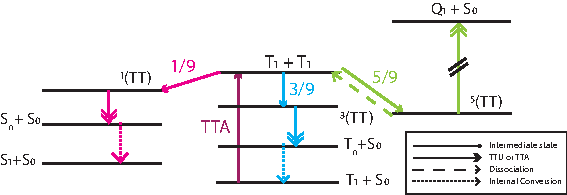
\includegraphics{./images/Asset 5.pdf}

}

\caption{Diagram illustrating the pathways of the triplet-triplet
upconversion process via triplet-triplet annihilation. The {1(TT)},
{3(TT)}, and {5(TT)} represent the singlet, triplet, and quintet
intermediate states.}

\end{figure}

\hypertarget{apen-dpaextra}{%
\section{2,6-DPA Neat Film extra pixels}\label{apen-dpaextra}}

\begin{figure}

\begin{minipage}[t]{0.50\linewidth}

{\centering 

\raisebox{-\height}{

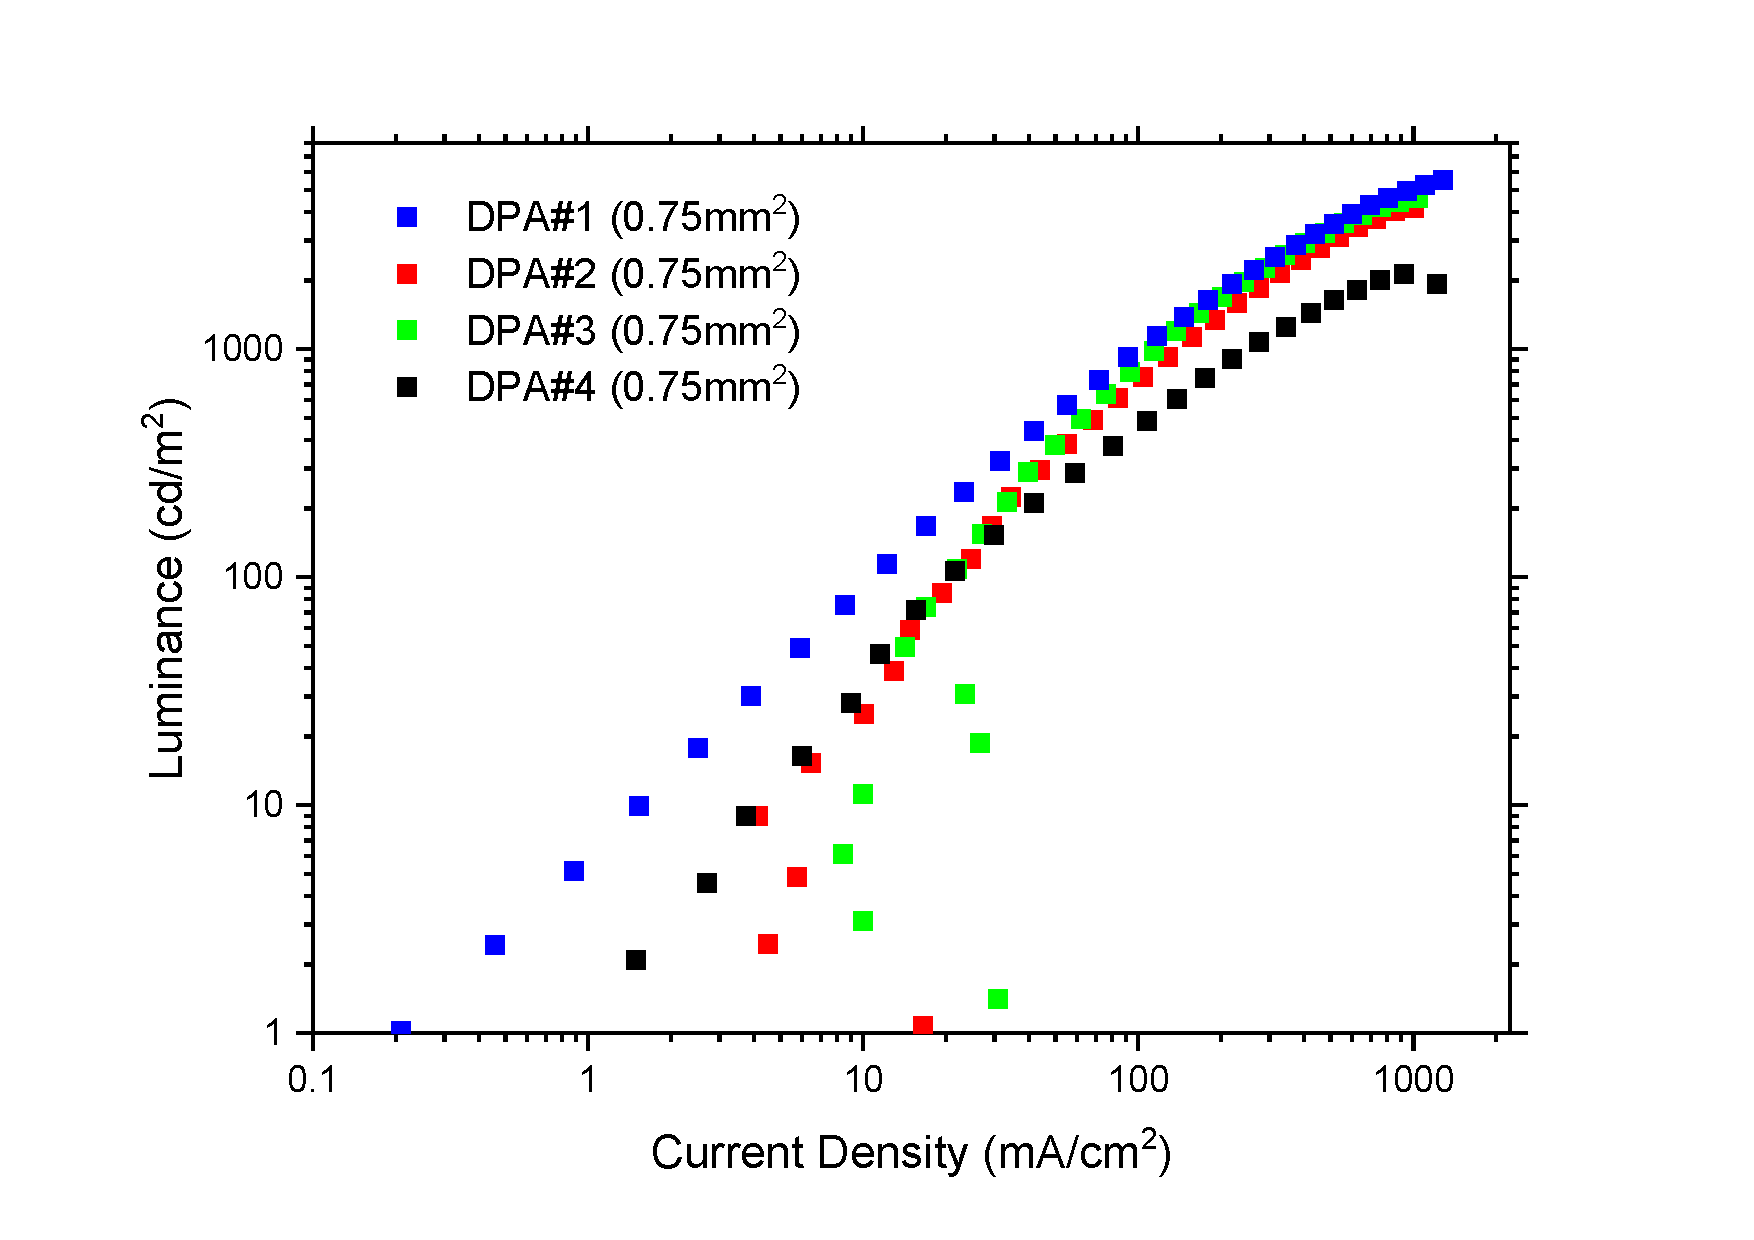
\includegraphics{./images/multijvldpa.pdf}

}

}

\subcaption{\label{fig-mjvl}}
\end{minipage}%
%
\begin{minipage}[t]{0.50\linewidth}

{\centering 

\raisebox{-\height}{

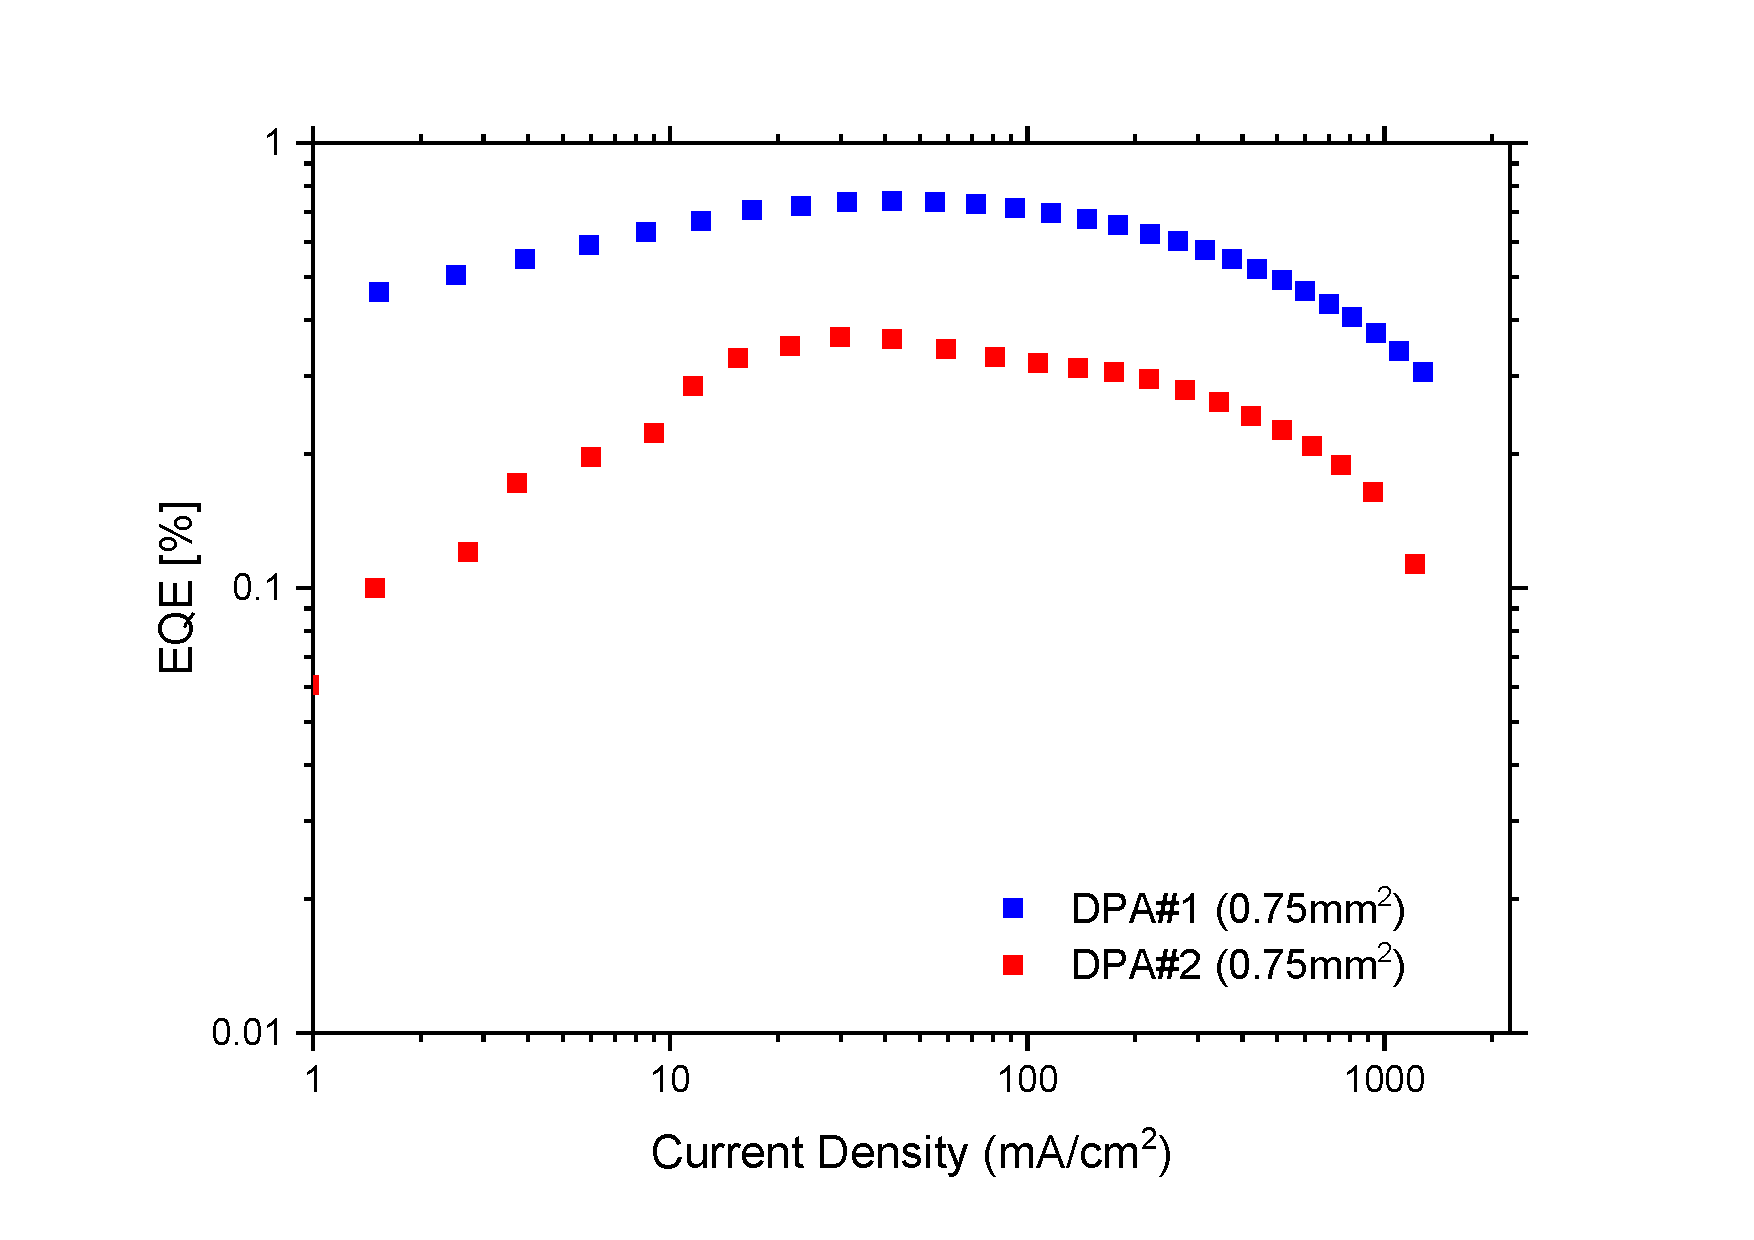
\includegraphics{./images/multiEQEdpa.pdf}

}

}

\subcaption{\label{fig-meqe}}
\end{minipage}%

\caption{\label{fig-multidpa}Current density-luminance-voltage (J-V-L)
graph of four different pixels (b) EQE versus current density graph for
two different pixels}

\end{figure}

\hypertarget{apen:oledex}{%
\section{TTU Confirmation OLED Structure}\label{apen:oledex}}

\begin{figure}

\begin{minipage}[t]{0.50\linewidth}

{\centering 

\raisebox{-\height}{

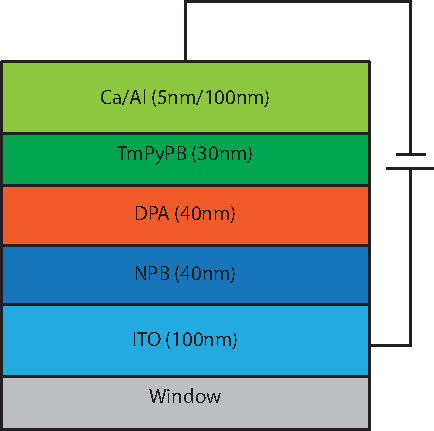
\includegraphics{./images/DPAOLED.pdf}

}

}

\subcaption{\label{fig-dpaoled}}
\end{minipage}%
%
\begin{minipage}[t]{0.50\linewidth}

{\centering 

\raisebox{-\height}{

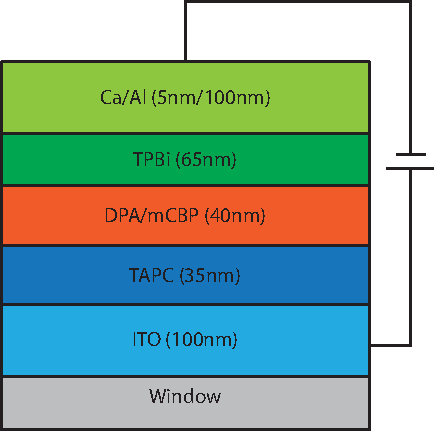
\includegraphics{./images/mCBPOLED.pdf}

}

}

\subcaption{\label{fig-mcbpoled}}
\end{minipage}%
\newline
\begin{minipage}[t]{\linewidth}

{\centering 

\raisebox{-\height}{

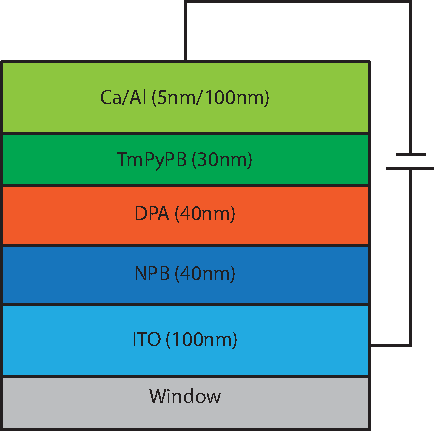
\includegraphics{./images/Coumarin6 OLED.pdf}

}

}

\subcaption{\label{fig-c6oled}}
\end{minipage}%

\caption{\label{fig-oledextra}Figure (a) Indium Tin Oxide (ITO) 100nm /
N,N'-Di(1-naphthyl)-N,N'-diphenyl-(1,1'-biphenyl)-4,4'-diamine (NPB)
40nm / 2,6-DPA 40nm / 1,3,5-Tris(3-pyridyl-3-phenyl)benzene (TmPyPB)
30nm / Calcium 5nm / Aluminum 100nm. (b) Indium Tin Oxide (ITO) 100nm /
1,1-Bis{[}(di-4-tolylamino)phenyl{]}cyclohexane (TAPC) 35nm /
2,6-DPA/mCBP (10wt\%) 40nm /
2,2',2''-(1,3,5-Benzinetriyl)-tris(1-phenyl-1-H-benzimidazole) (TPBi)
65nm / Calcium 5nm / Aluminum 100nm}

\end{figure}



\end{document}
